% !TeX root = d2.tex

\documentclass{article}

% \usepackage{xcolor}
\usepackage[margin=0.5in]{geometry} 
\usepackage{graphicx}
\usepackage{multirow}
\usepackage[table,xcdraw]{xcolor}
\usepackage[normalem]{ulem}
\usepackage{float}
\usepackage{adjustbox, lipsum}
\usepackage{pdfpages}
\useunder{\uline}{\ul}{}
\title{MindMerge --- Deliverable e 2}
\author{Gabriele Benetti, Gioele Bernardini, Luca Fossa Crescini, Luca Sartore}

\begin{document}
\maketitle


\tableofcontents


\newpage
\section*{Abstract}   % titolo temporaneo da modificare
This is the Abstract of the deliverable 2

\section{Architecture description}


\begin{figure}[h]
  \centering
  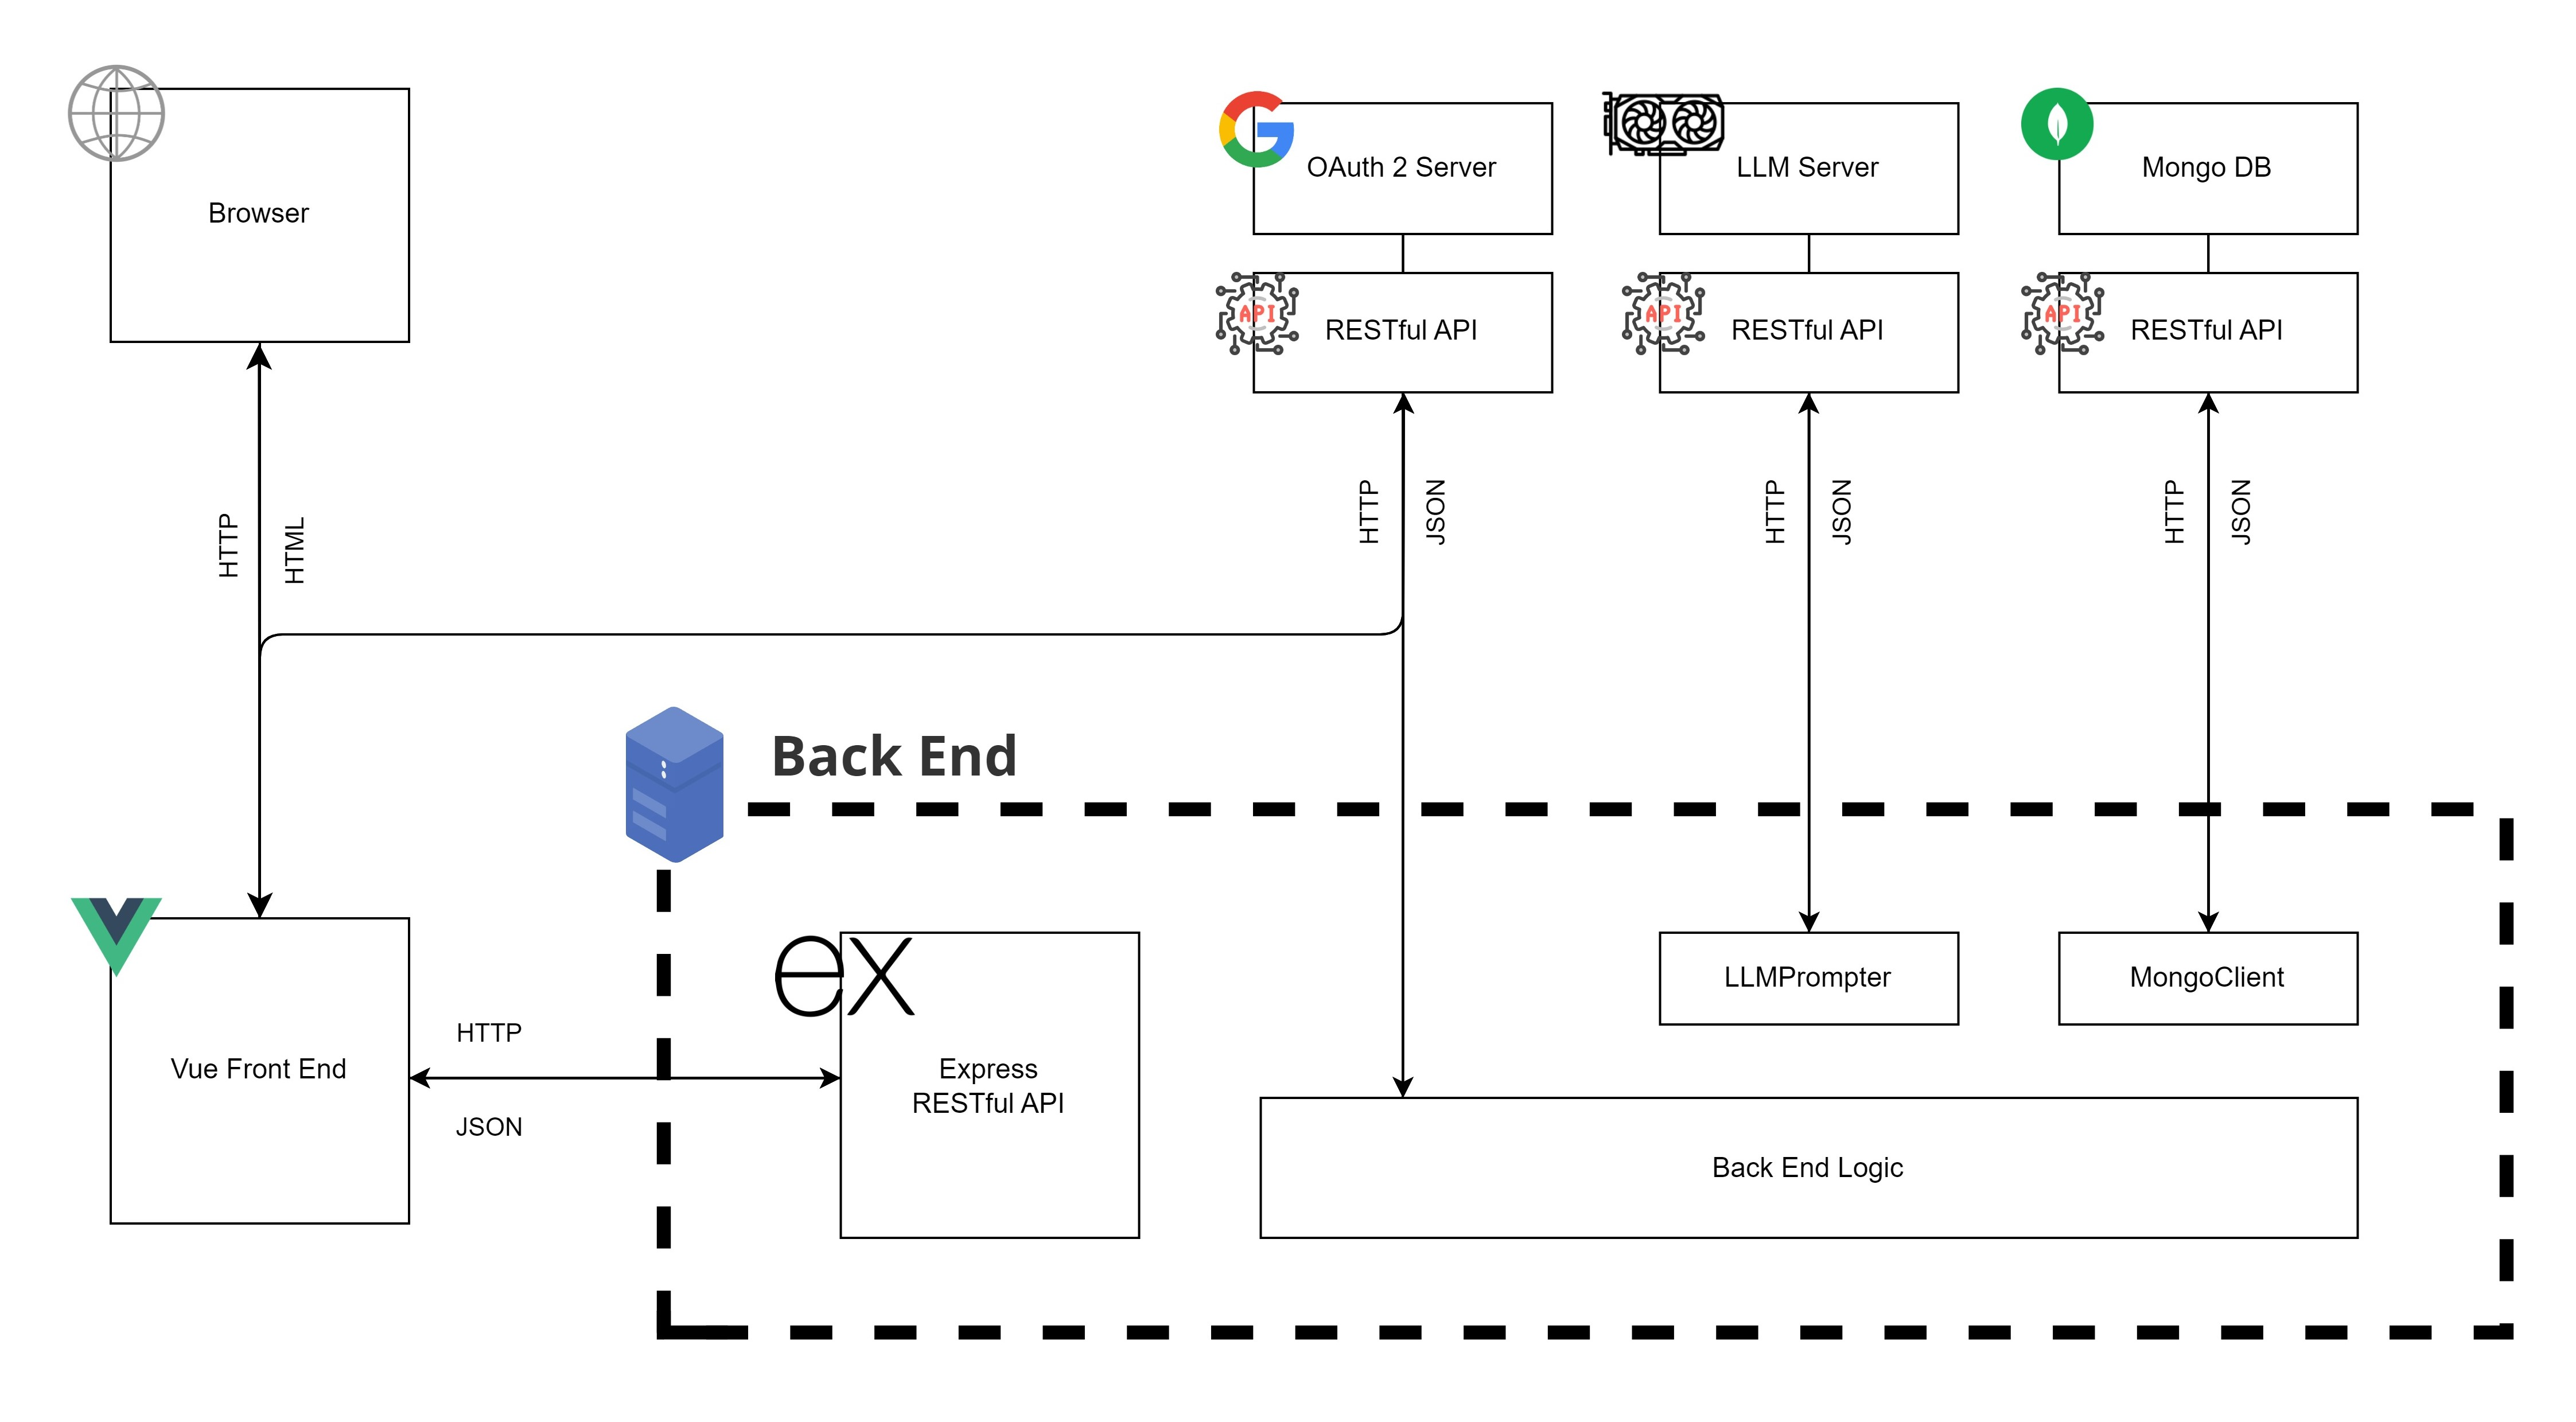
\includegraphics[width=0.95\textwidth]{images/architecture.jpg}
  \caption{\small The architecture diagram ot the MindMerge system}
\end{figure}
The architecture is relatively simple,
comprising two classical components: the front end and the back end, along with several smaller components (browser, OAuth server, LLM service, and MongoDB).
\newline \newline
The browser communicates with the front end using the HTTP protocol and HTML format.
\newline \newline
The front end, based on the Vue library, accesses resources provided by the back end using HTTP with JSON data format.
\newline \newline
Authentication is provided by a third-party OAuth server, that communicate with both the front end and back end via HTTP/JSON.
\newline \newline
The back end is the most complex component consists of several sub-components, including:
\begin{itemize}
  \item A part providing RESTful APIs based on Express.js
  \item A component dedicated to communicating with the database (MongoClient)
  \item A module for communicating with the LLM service (LLMPrompter)
  \item Logic containing all functions necessary for the application's operation.
\end{itemize}
All the communications that the backend has with the external world are made through HTTP with json format.
\newpage
\section{Product Backlog}

This section contains the product backlogs we have built during our development process.
There are a few differences between the various versions. The most obvious one is that we added a new colum
every time to represent the estimated effort that remained for every task. As well as some changes to the descriptions;
for example, we realized after we began the first sprint that we missed the ``so that..'' part of the user stories.
Therefore, we added it in the following versions.\newline
The complete list of all the product backlog we submitted, as well as the time they were written, is as follows:

\begin{itemize}
  \item \textbf{Version 1.0:} The initial product backlog, that was written before the sprint 1.
  \item \textbf{Version 2.0:} The second product backlog, tha was written between the sprint 1 and the sprint 2.
  \item \textbf{Version 3.0:} The third product backlog, that was written between the sprint 2 and the sprint 3.
  \item \textbf{Version 4.0:} The fourth product backlog, that was written at the end of the third sprint.
\end{itemize}
\subsection{Version 1.0}
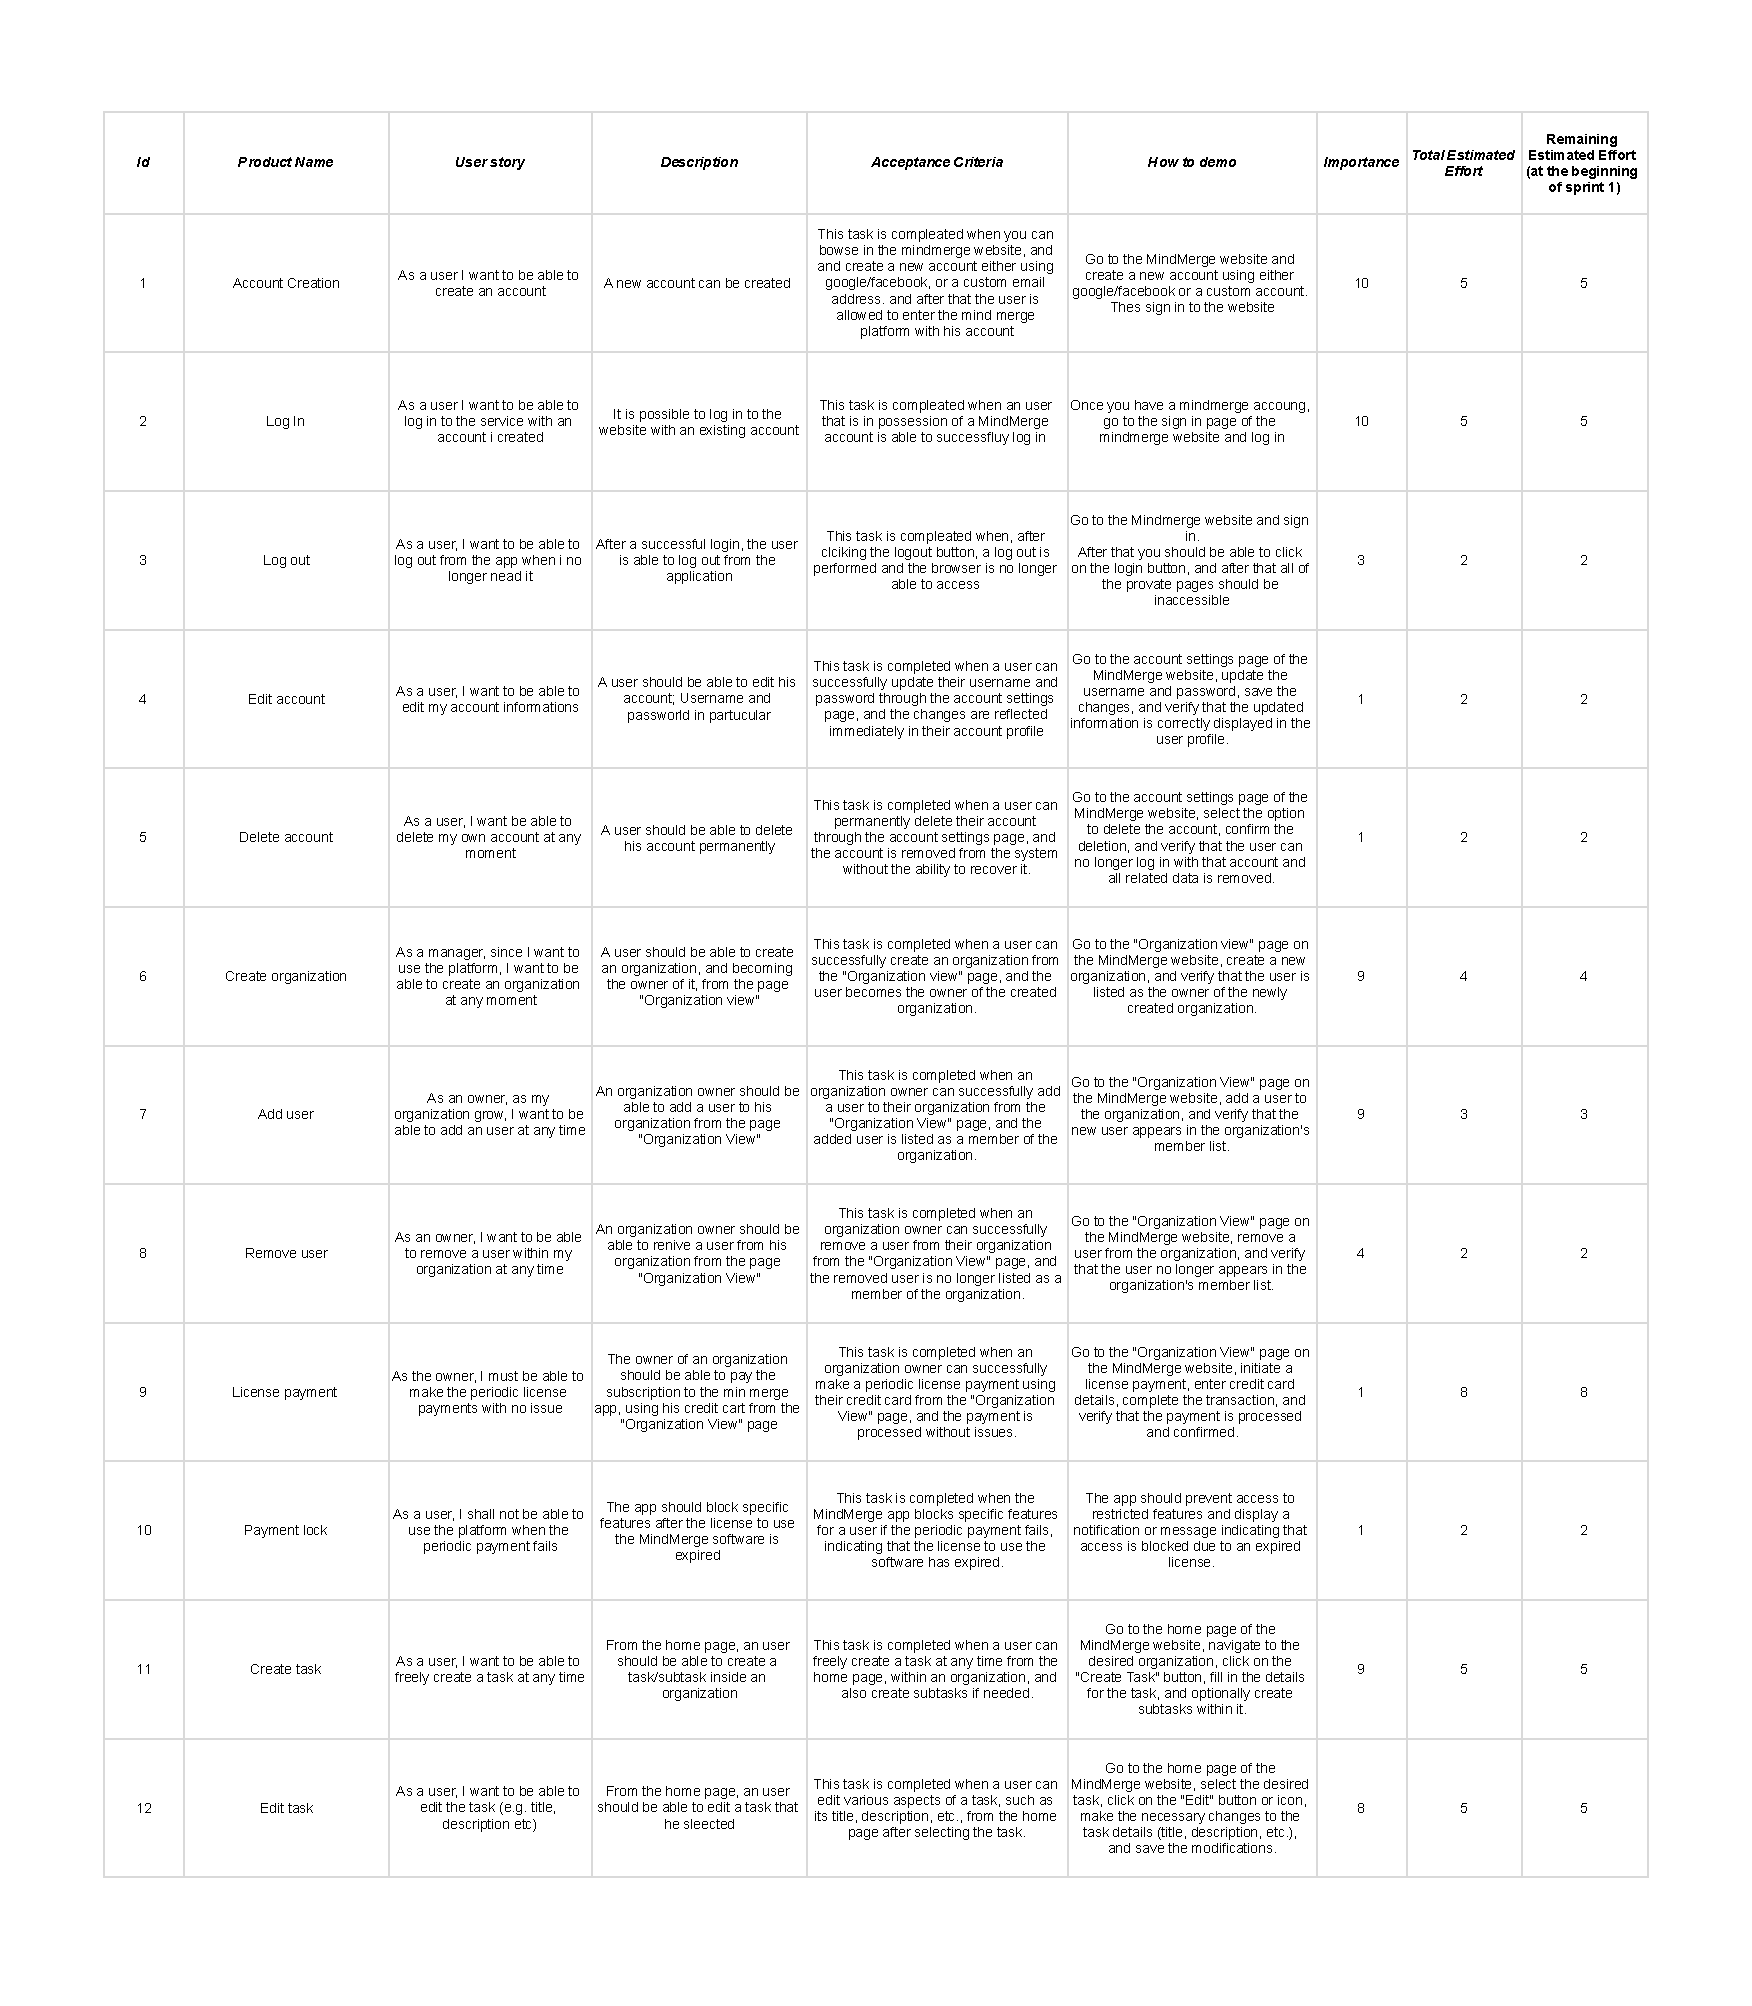
\includepdf[pages=-]{images/product_backlog_v1.pdf}
\subsection{Version 2.0}
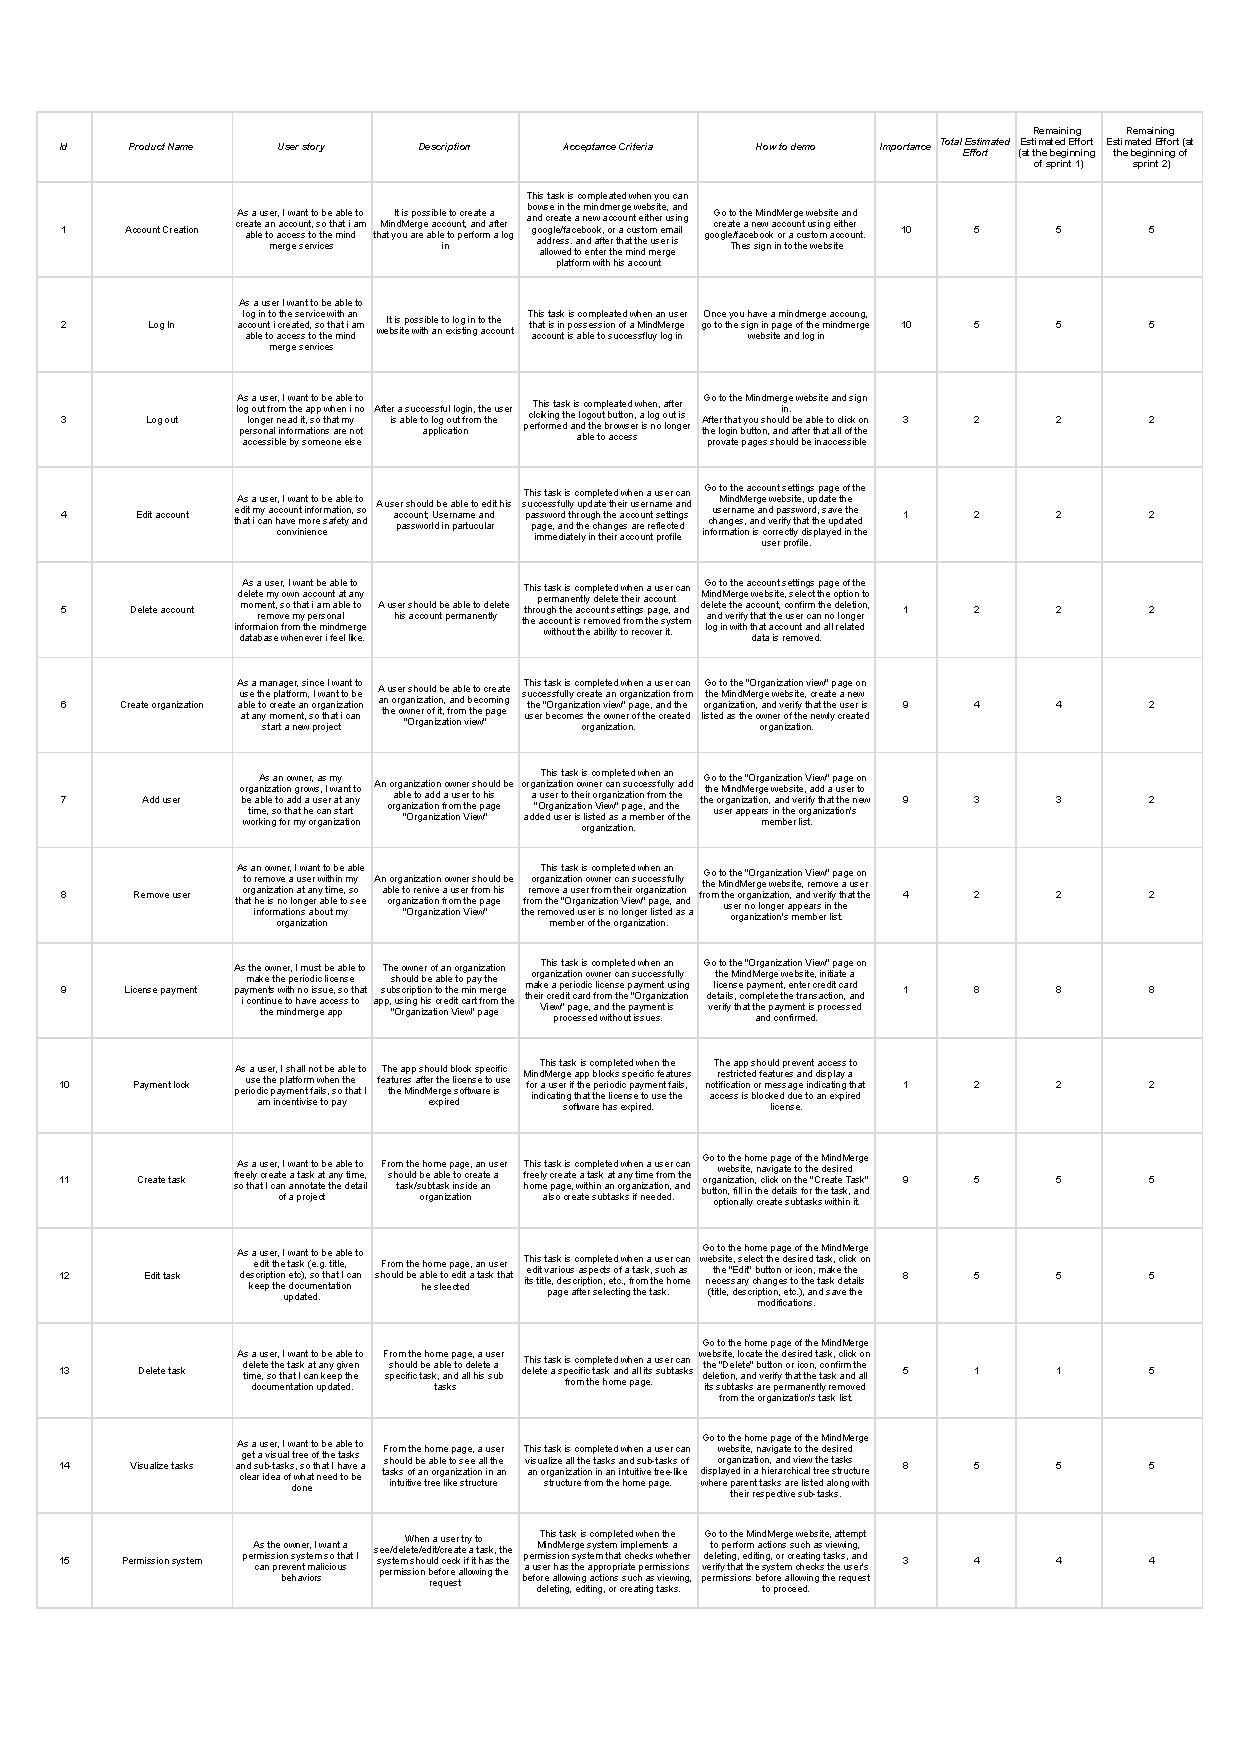
\includepdf[pages=-]{images/product_backlog_v2.pdf}
\subsection{Version 3.0}
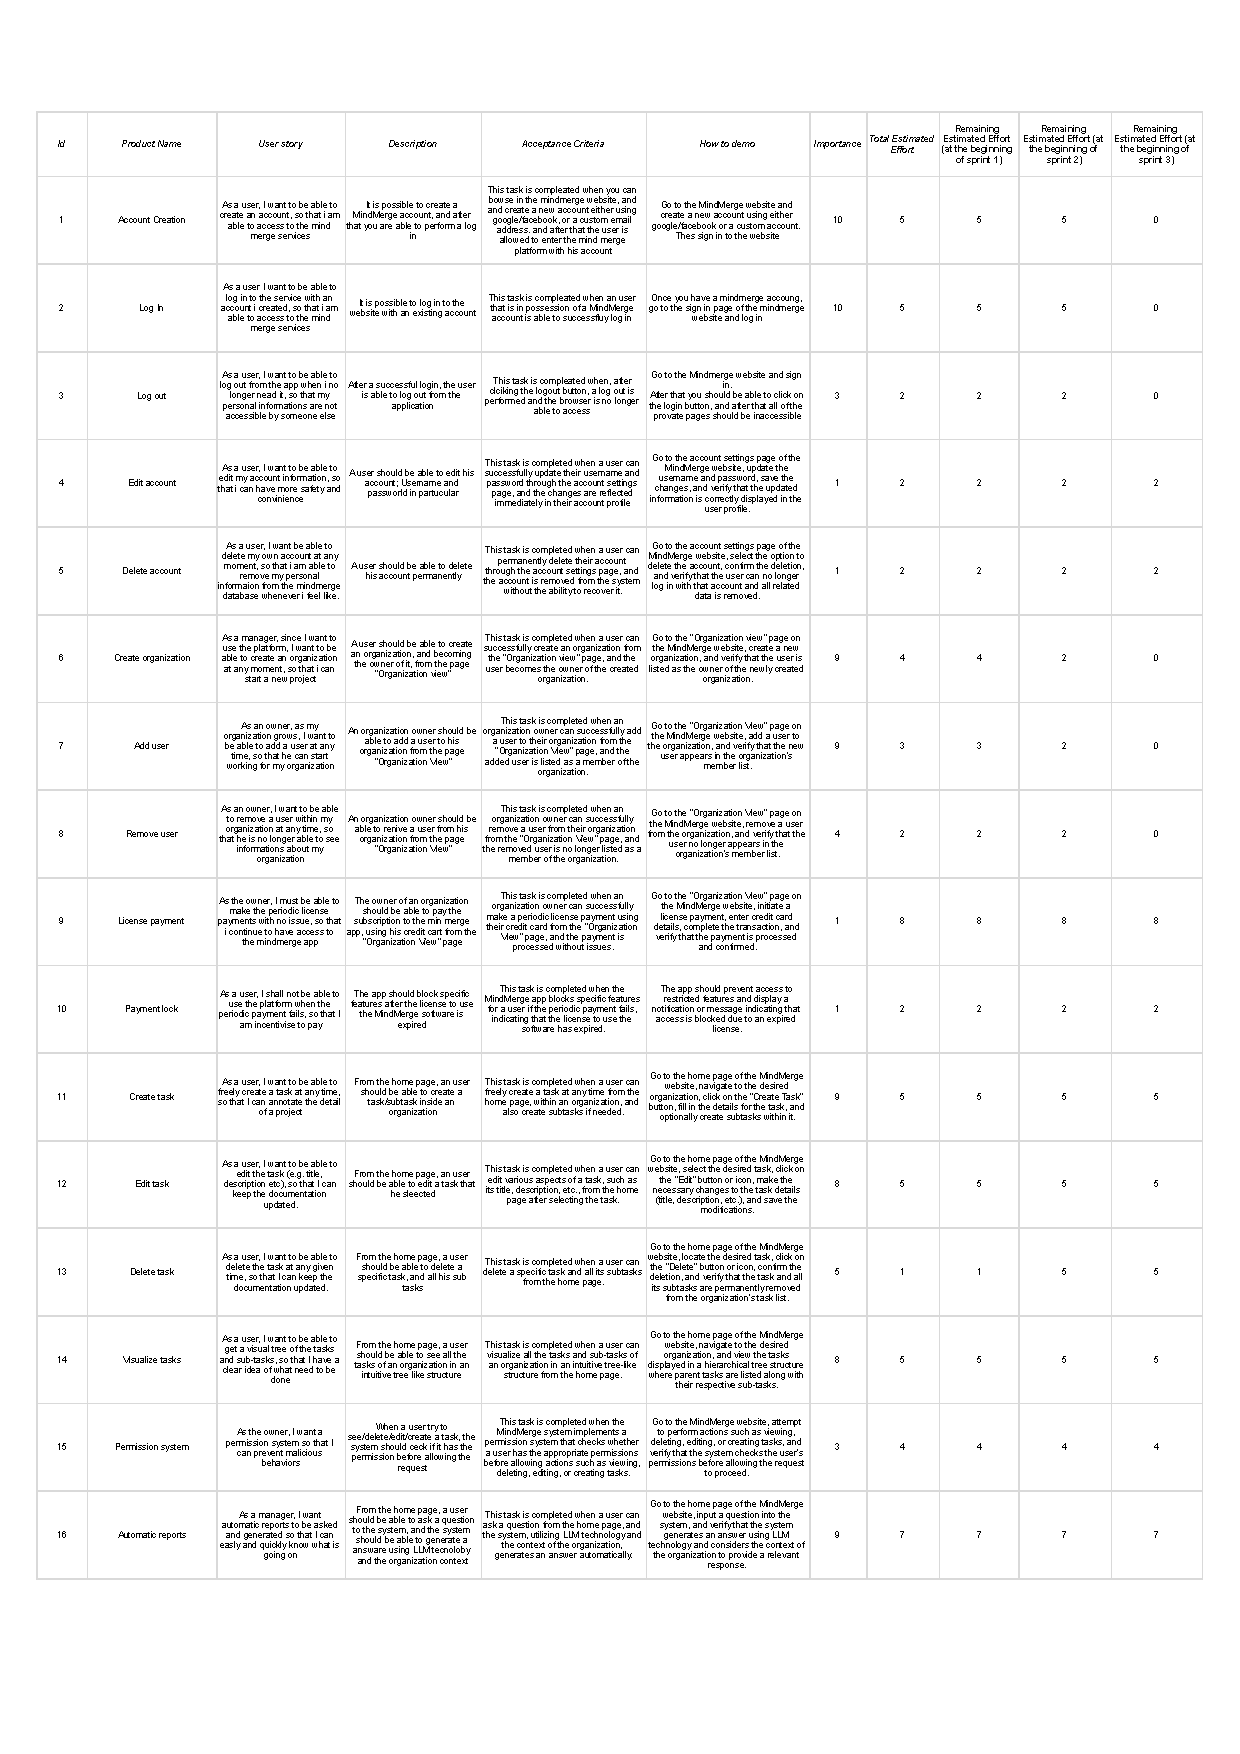
\includepdf[pages=-]{images/product_backlog_v3.pdf}
\subsection{Version 4.0}
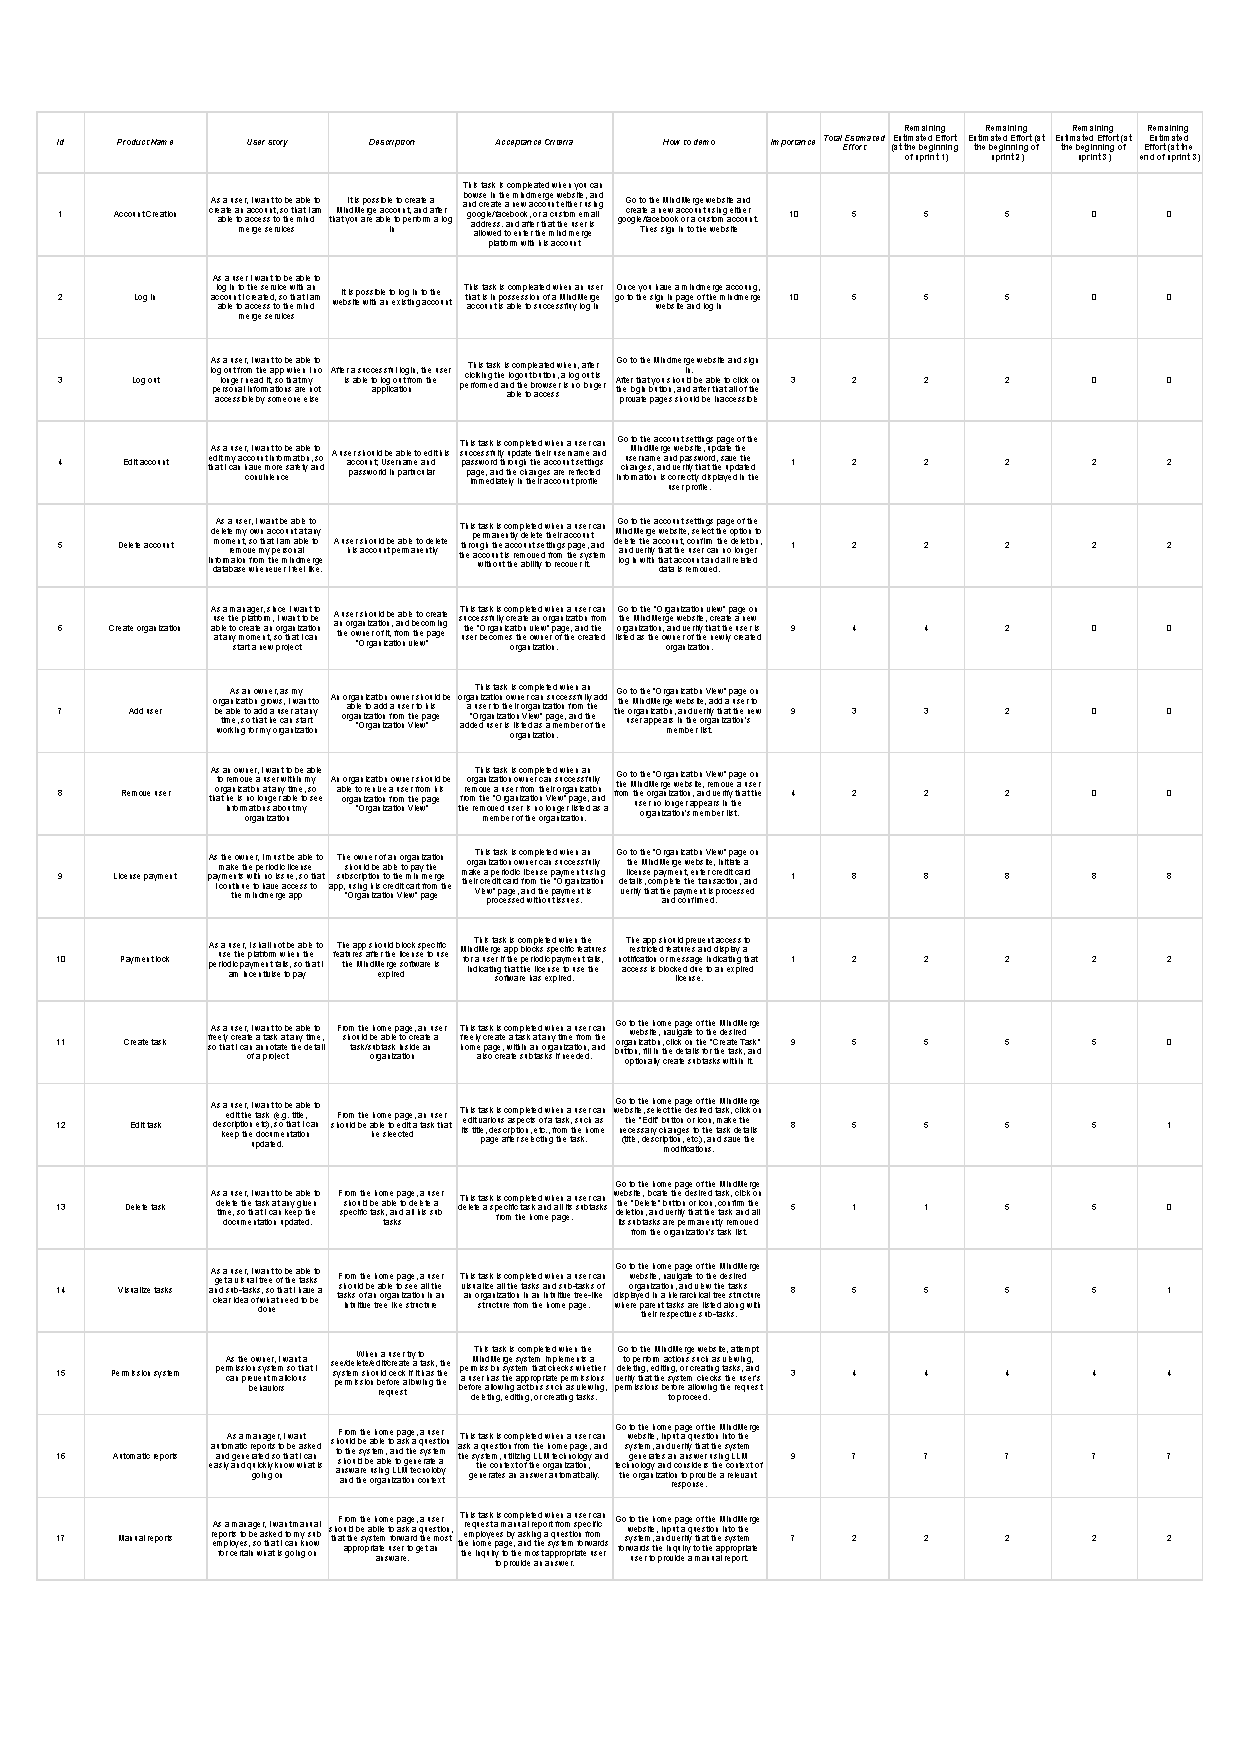
\includepdf[pages=-]{images/product_backlog_v4.pdf}


\section{Definition of Tests}

\subsection*{Test DatabaseManager:TaskManager}
This section contains the tests for the TaskManager class, which is responsible for managing tasks in the database.
\newline
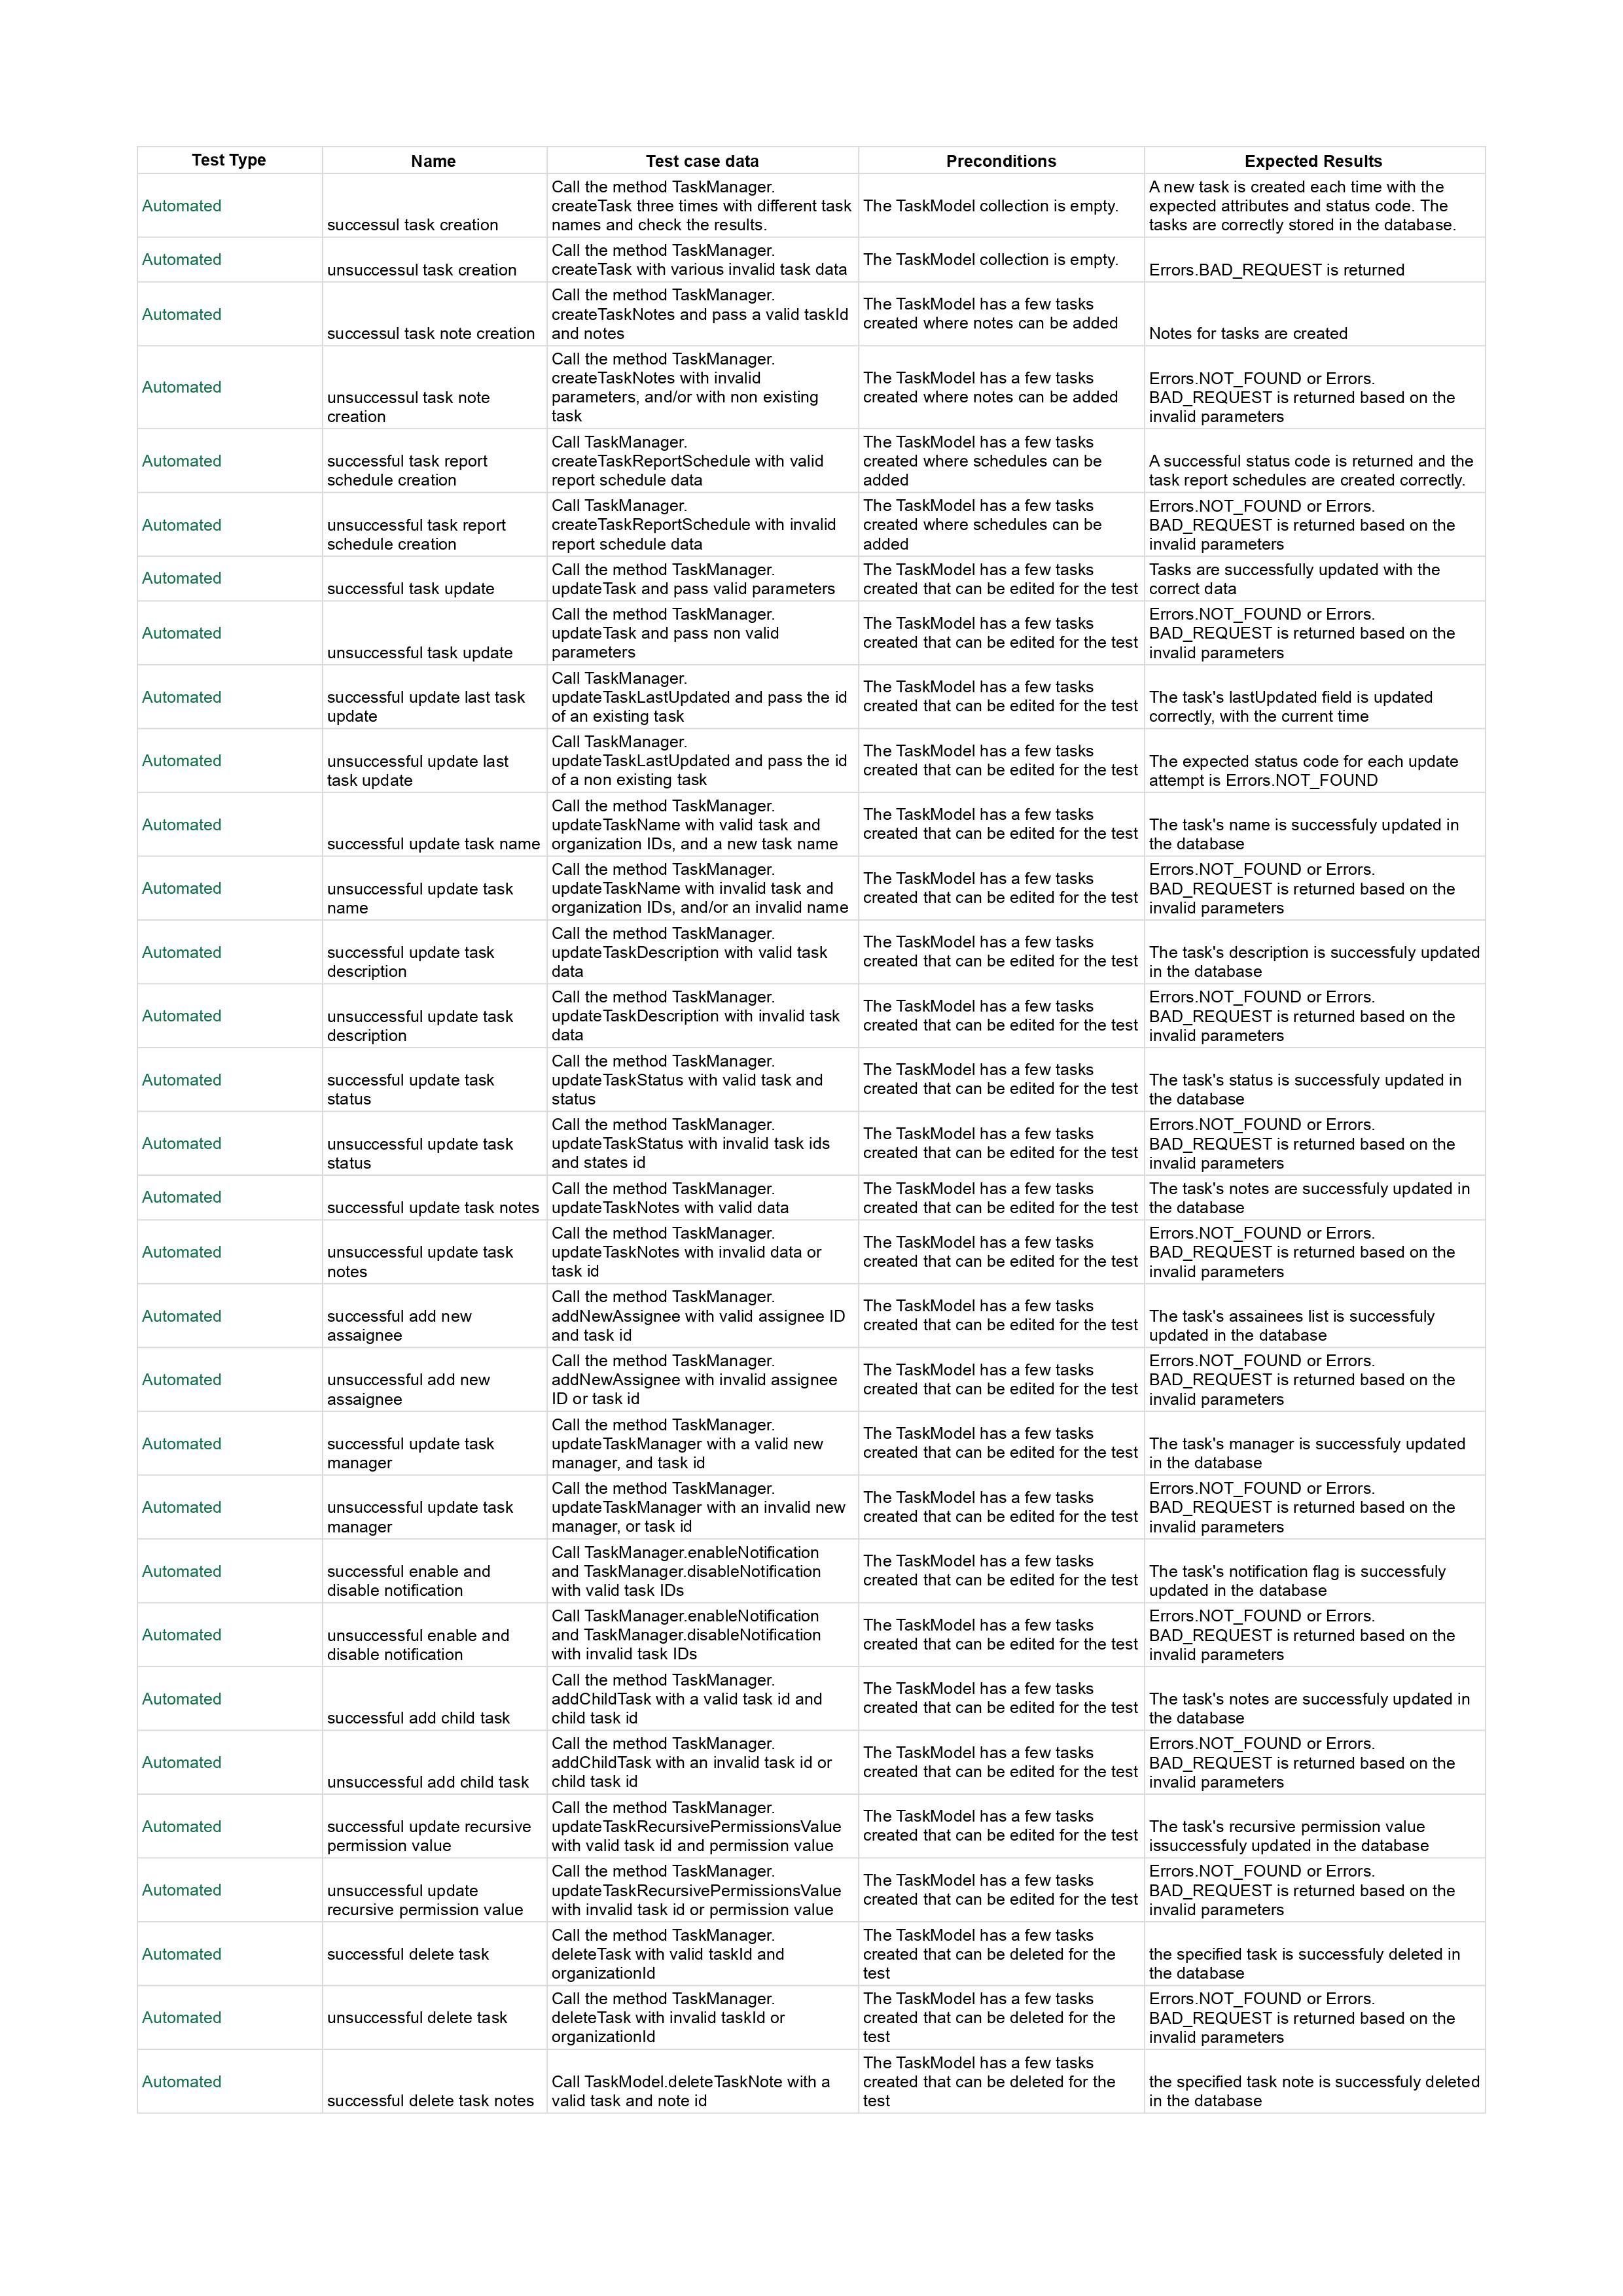
\includegraphics[width=0.95\textwidth]{images/Test_DatabaseManagerTaskManager-immagini-0.jpg}
\newline
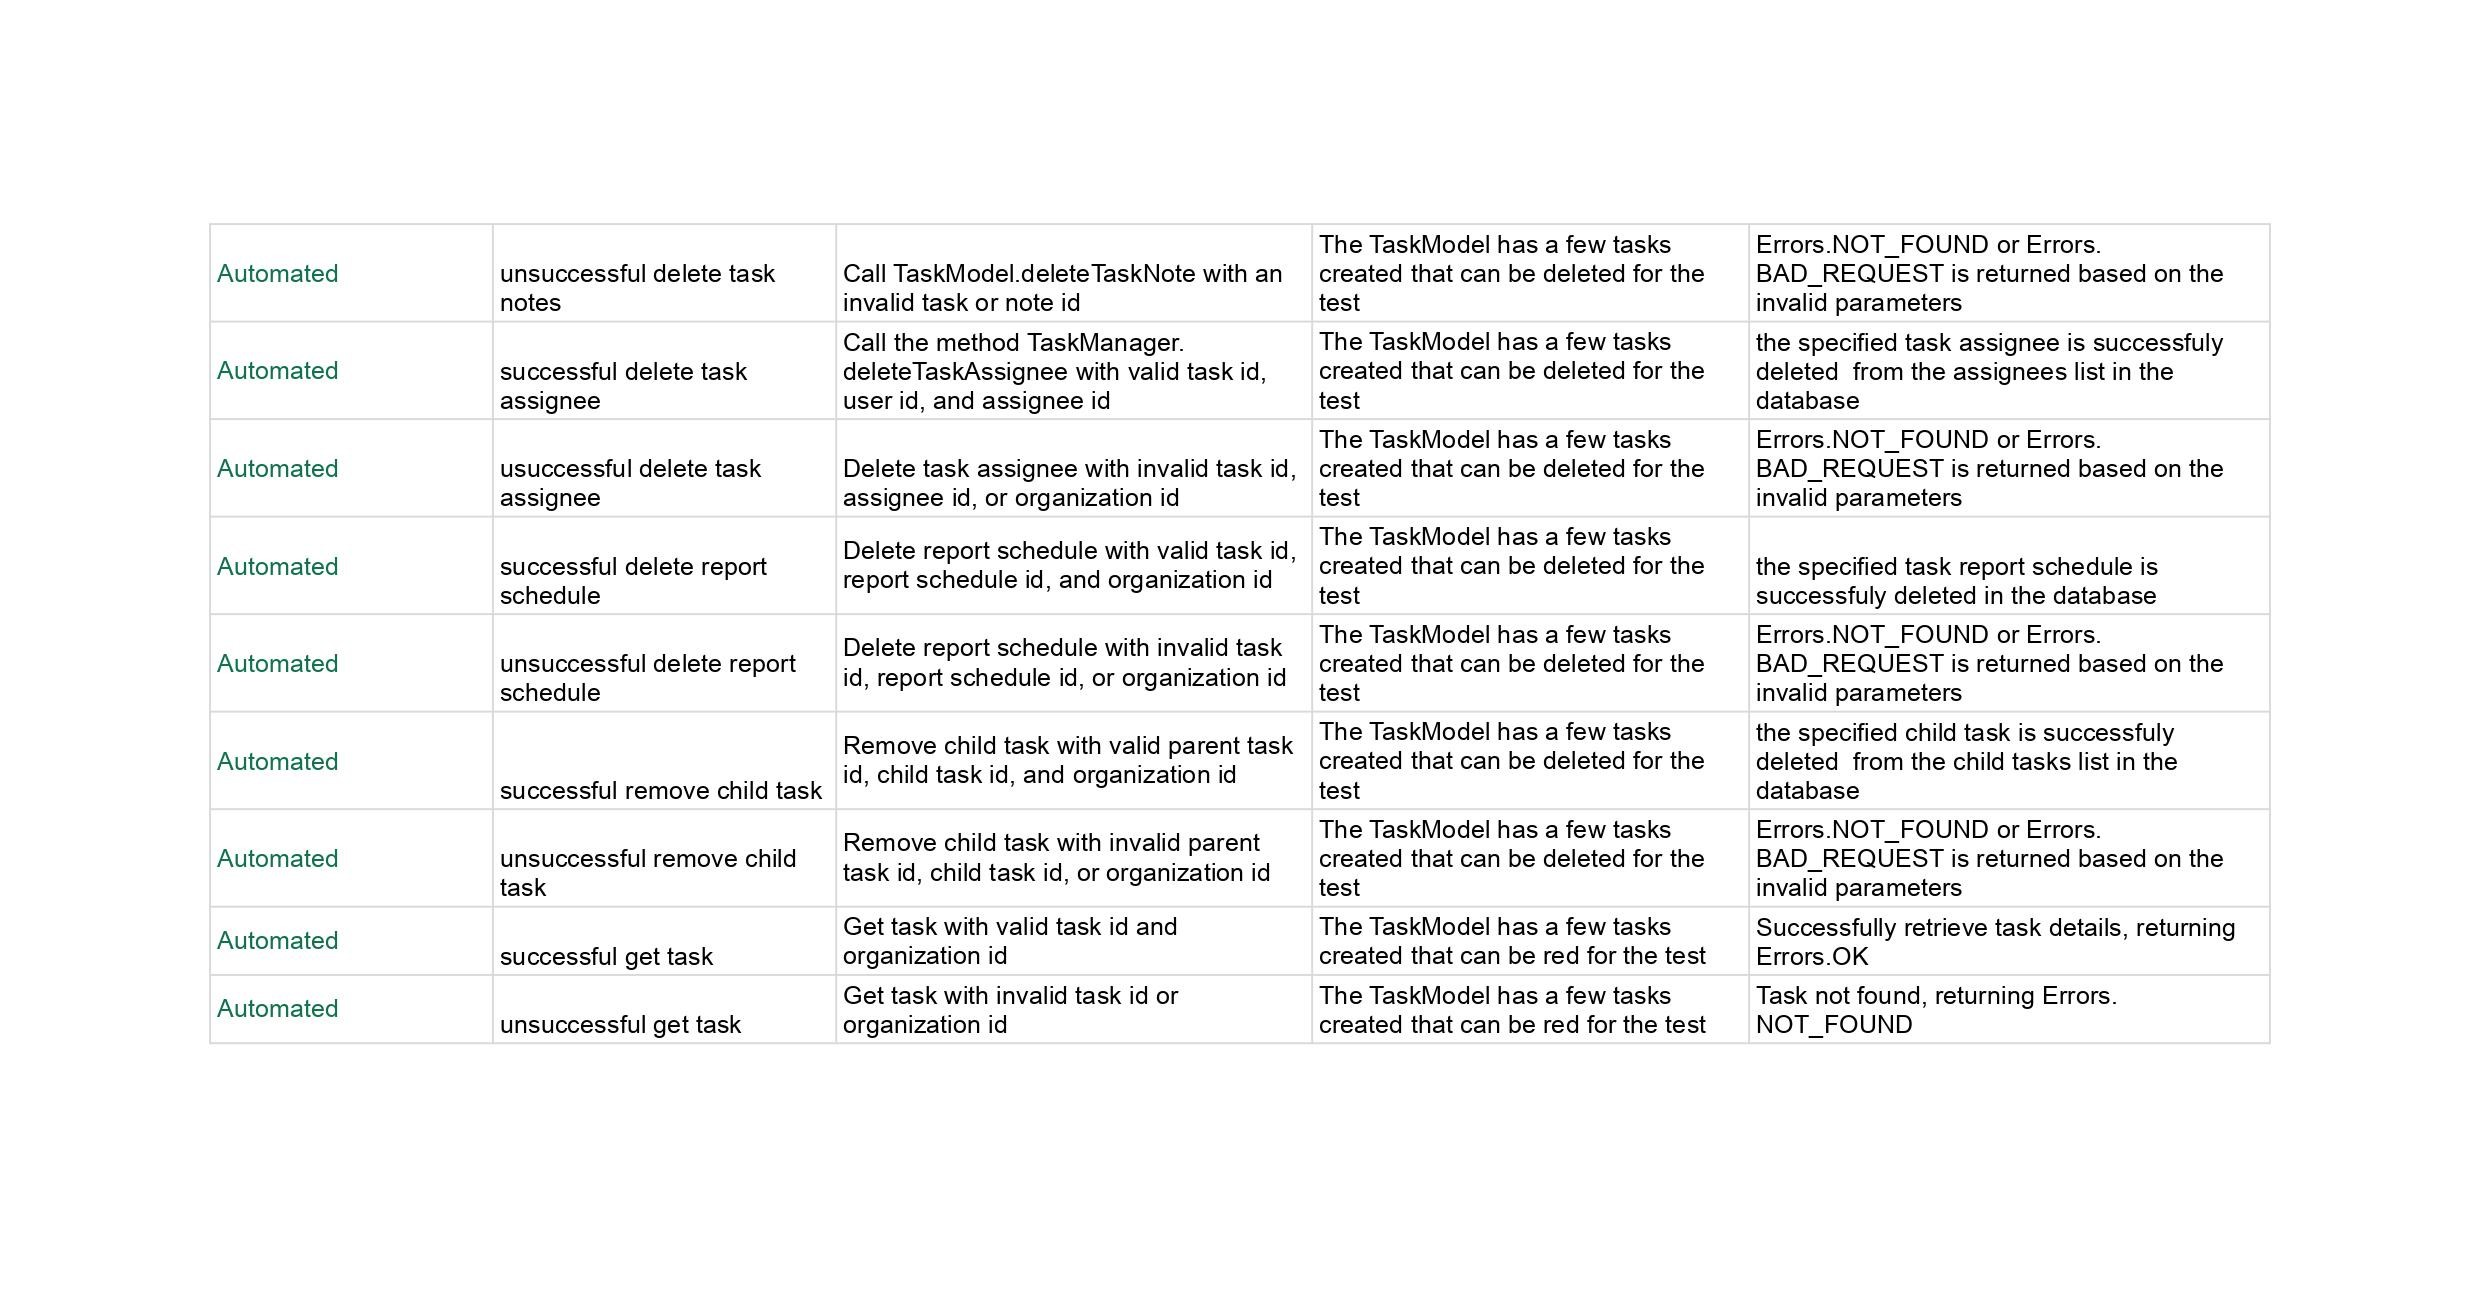
\includegraphics[width=0.95\textwidth]{images/Test_DatabaseManagerTaskManager-immagini-1.jpg}
\subsection*{Test OrganizationManager}
This section is dedicated to the tests for the OrganizationManager class, which is responsible for managing organizations in the database, with the integrated API.
\newline
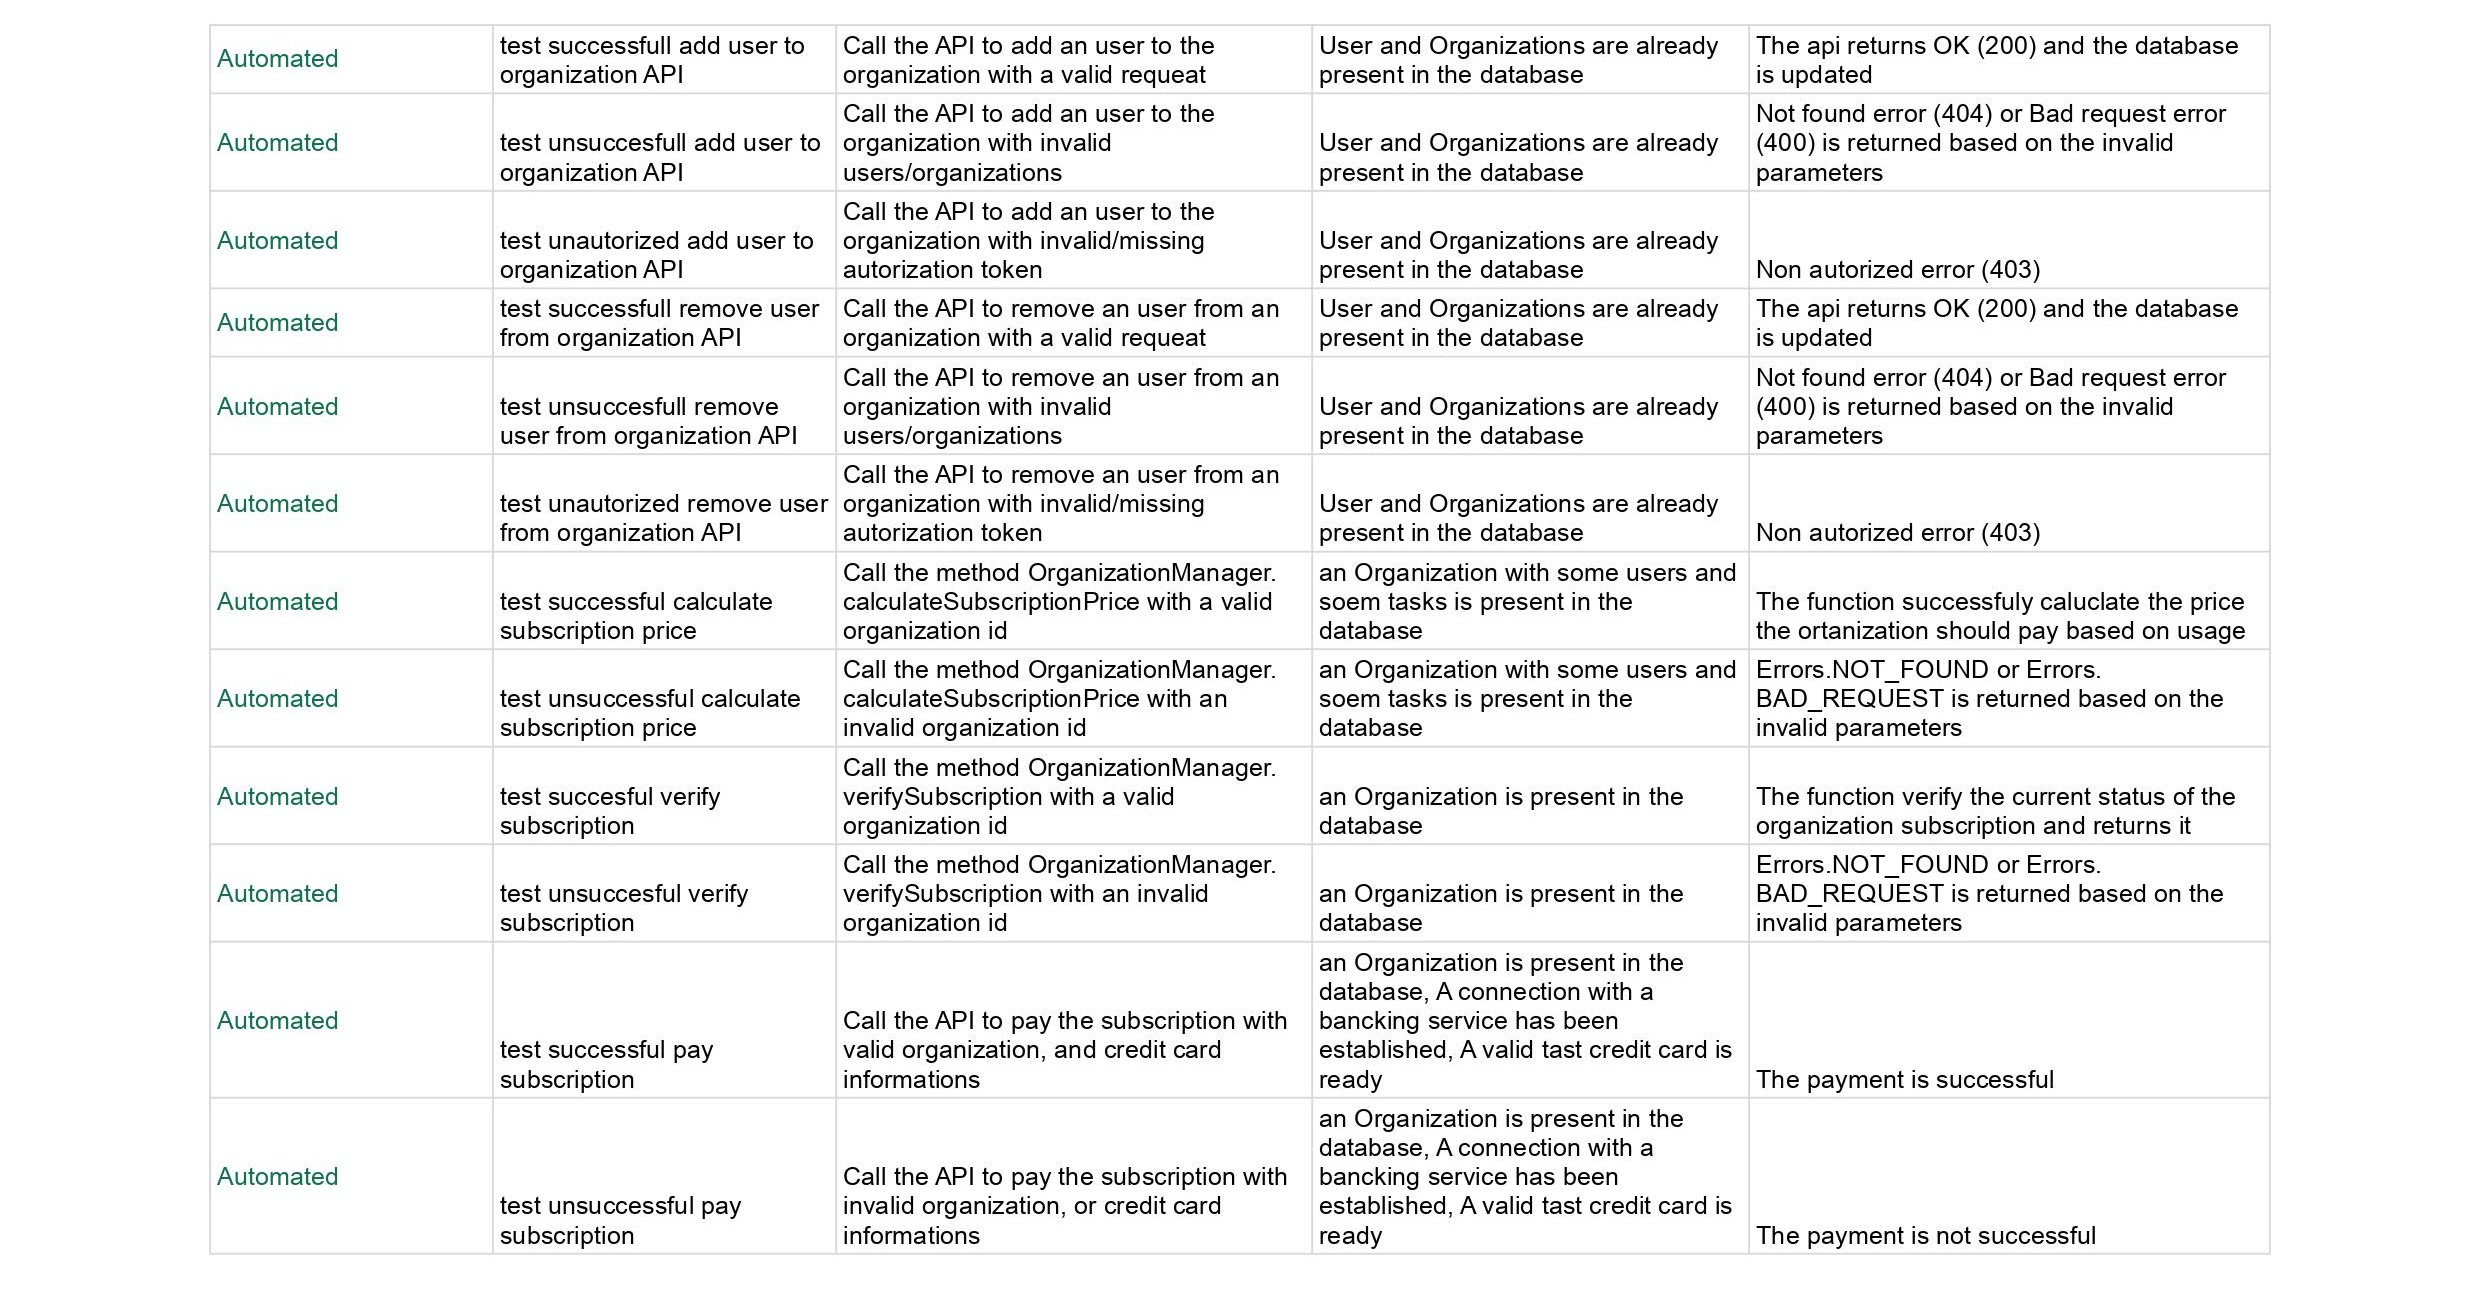
\includegraphics[width=0.95\textwidth]{images/Test_OrganizationManager.jpg}

\subsection*{Test Report Page}
This section includes manual tests for the Report Page, which is responsible for generating reports.
\newline
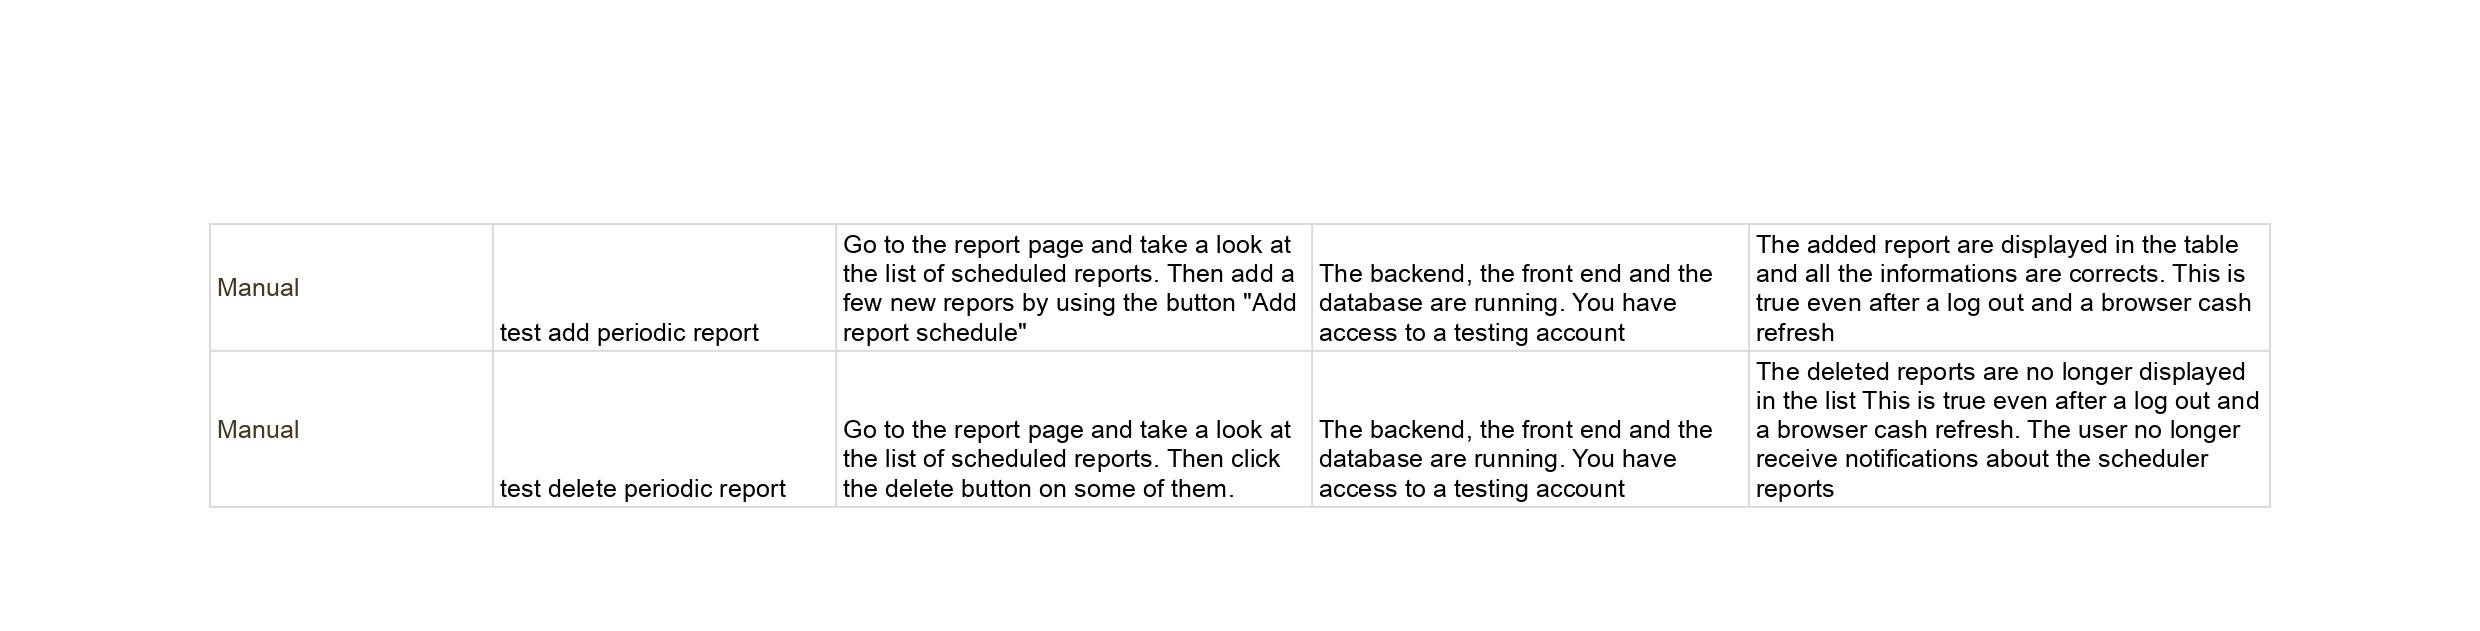
\includegraphics[width=0.95\textwidth]{images/Test_ReportPage.jpg}
\subsection*{Test NotificationManager}
This section includes automated tests for the NotificationManager class, which is responsible for managing notifications in the database.
\newline
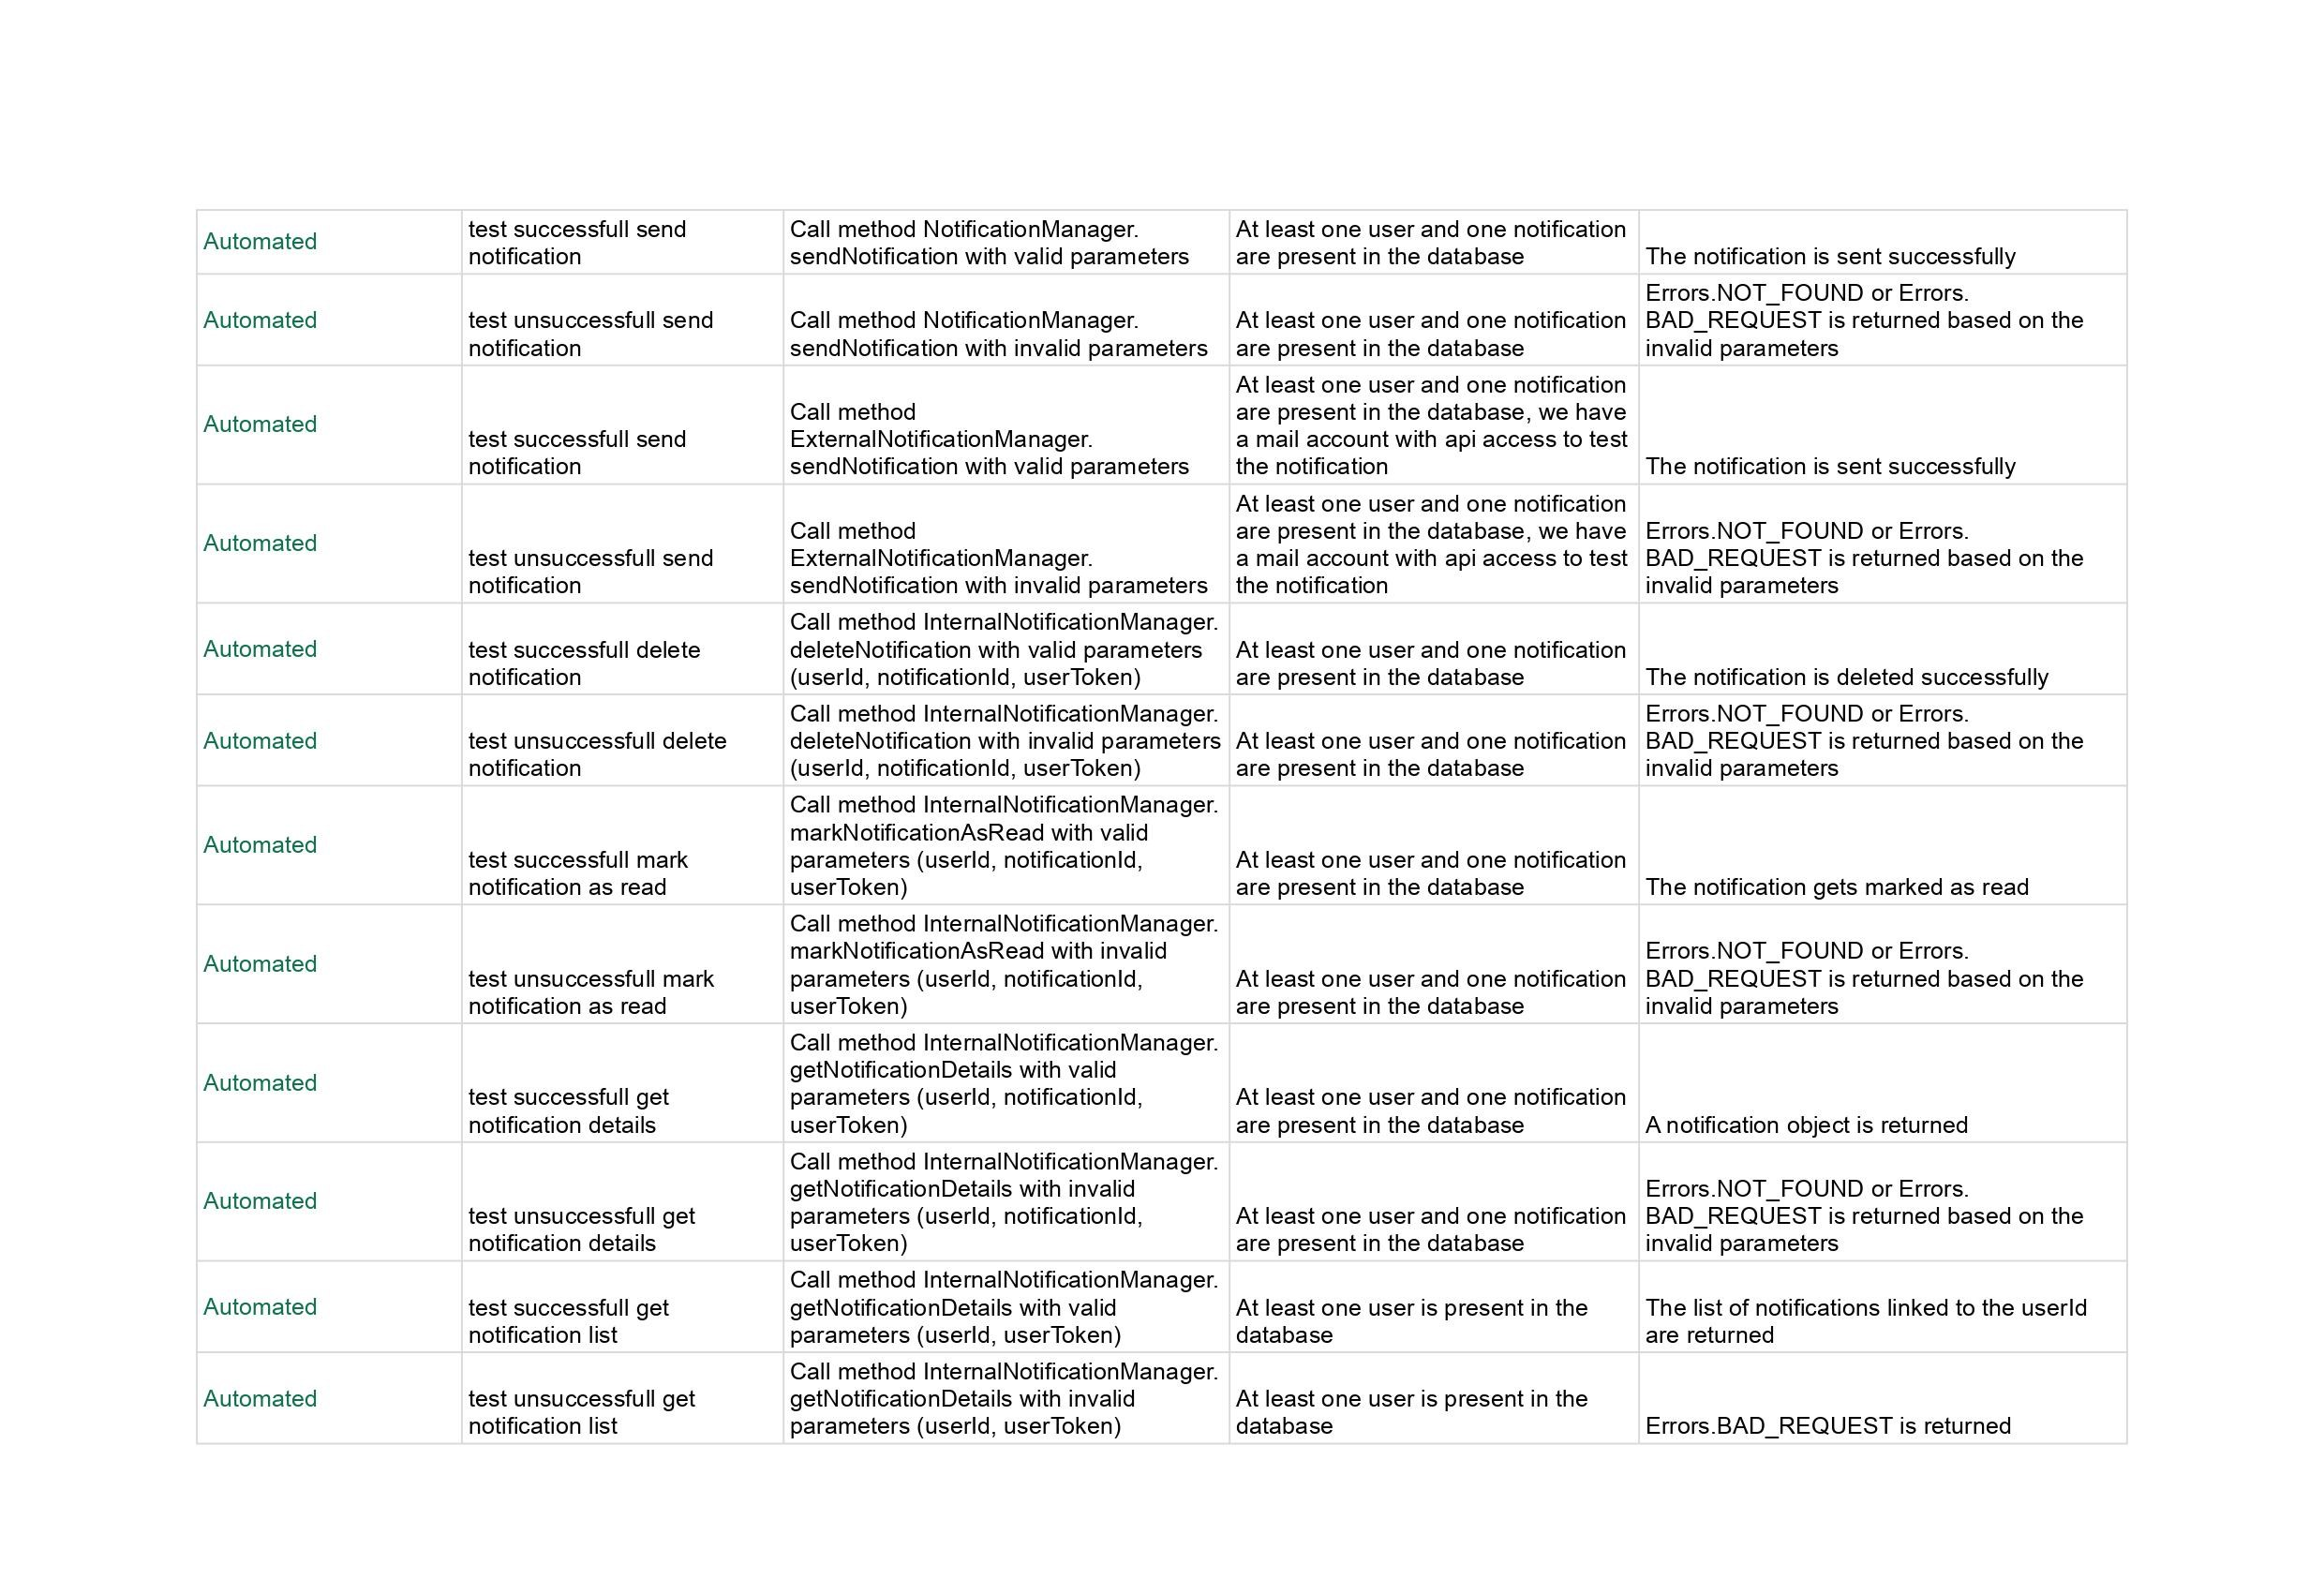
\includegraphics[width=0.95\textwidth]{images/Test_NotificationManager.jpg}

\subsection*{Test ReportManager}
This section includes automated tests for the ReportManager class, which is responsible for managing reports in the database.
\newline
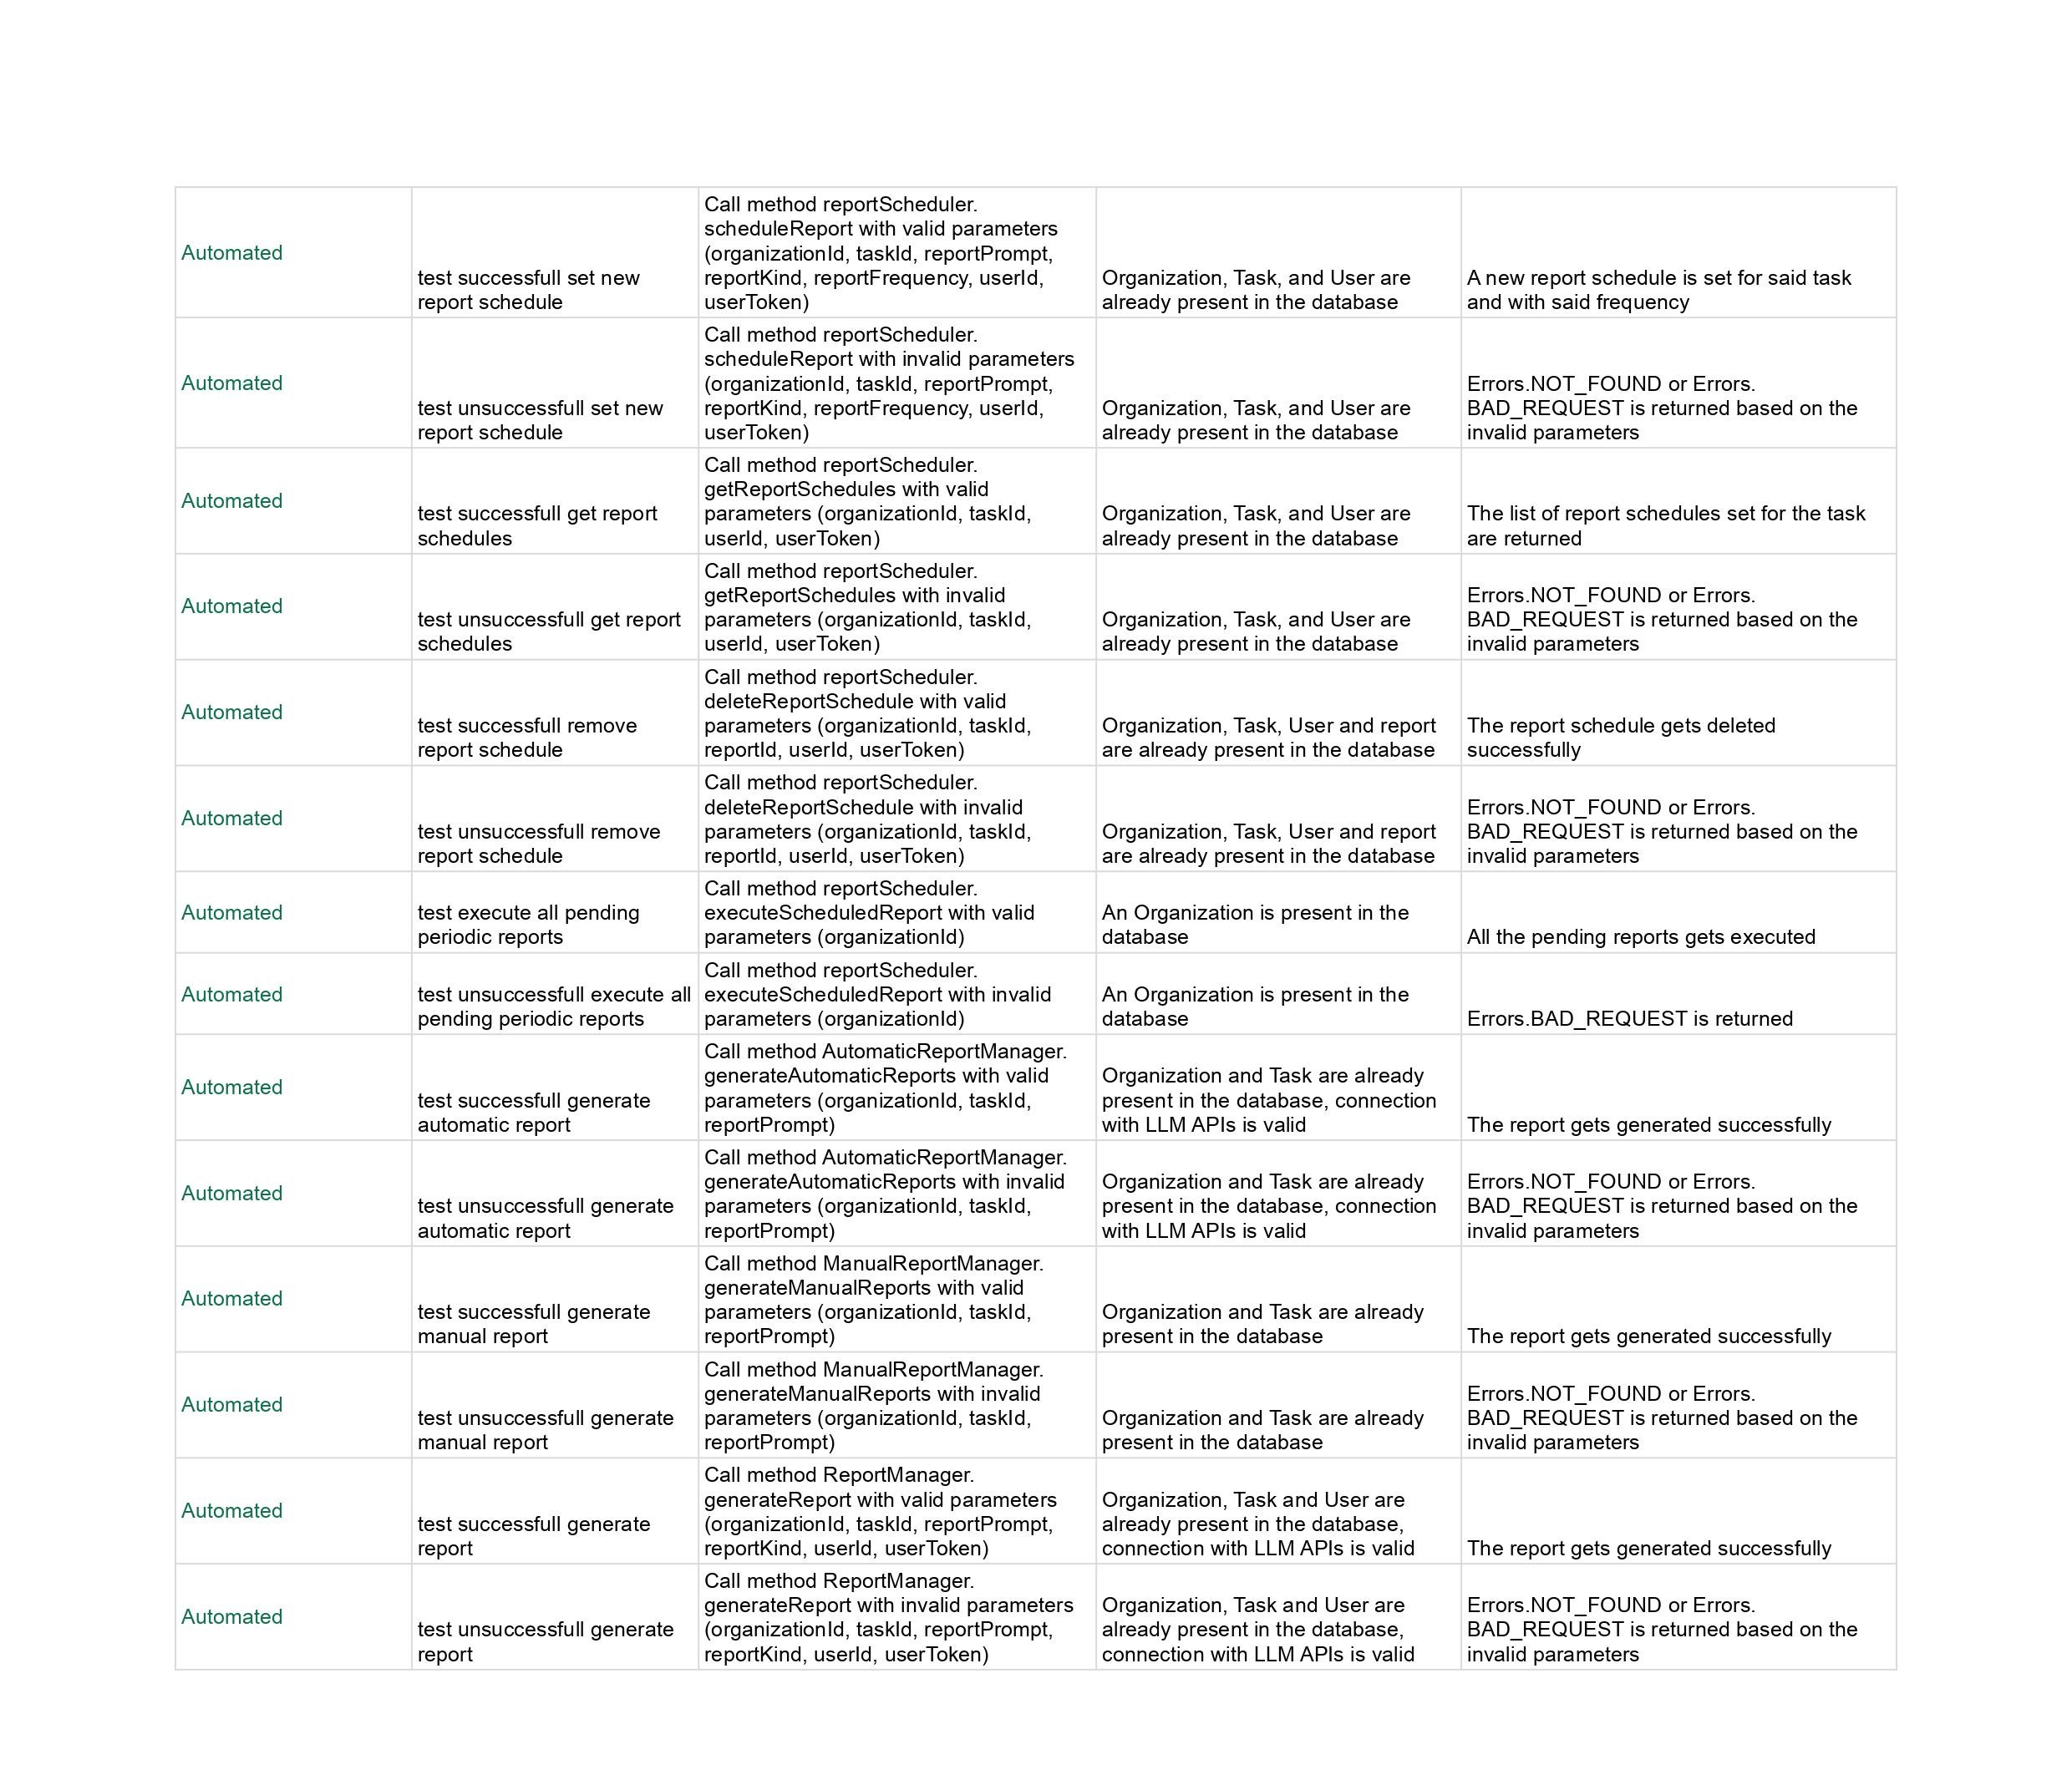
\includegraphics[width=0.95\textwidth]{images/Test_ReportManager.jpg}

\subsection*{Test DatabaseManager::OrganizationManager}
This section is dedicated to the tests for the OrganizationManager class, which is responsible for managing organizations in the database.
\newline
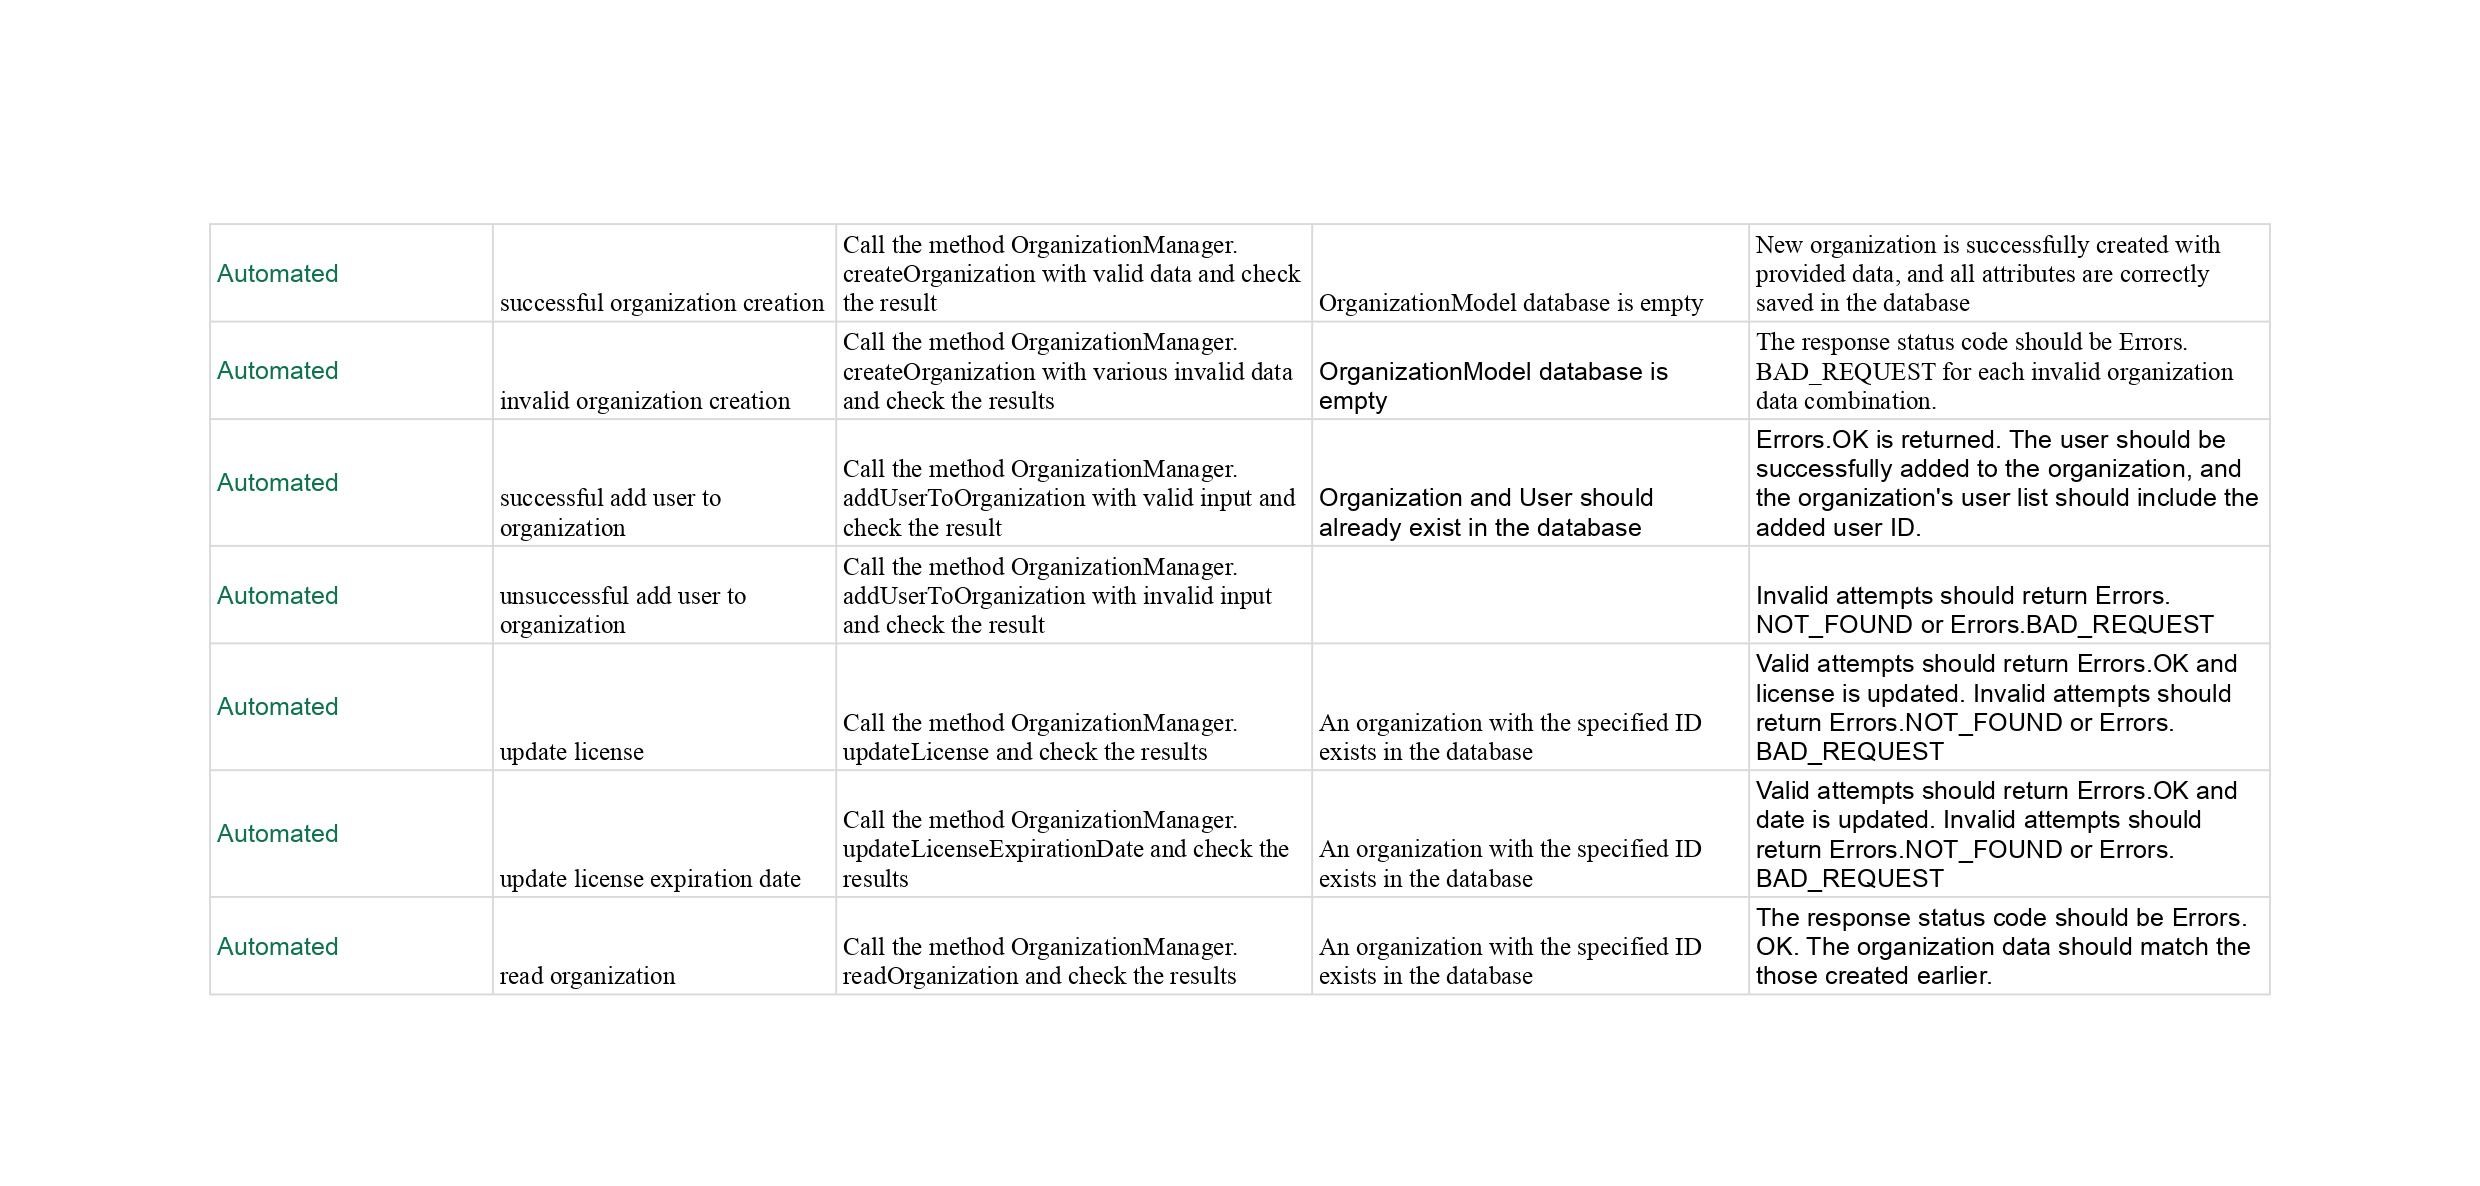
\includegraphics[width=0.95\textwidth]{images/Test_DatabaseManagerOrganizationManager.jpg}

\subsection*{Test AccountManager}
This section includes automated tests for the AccountManager class, which is responsible for managing accounts in the database.
\newline
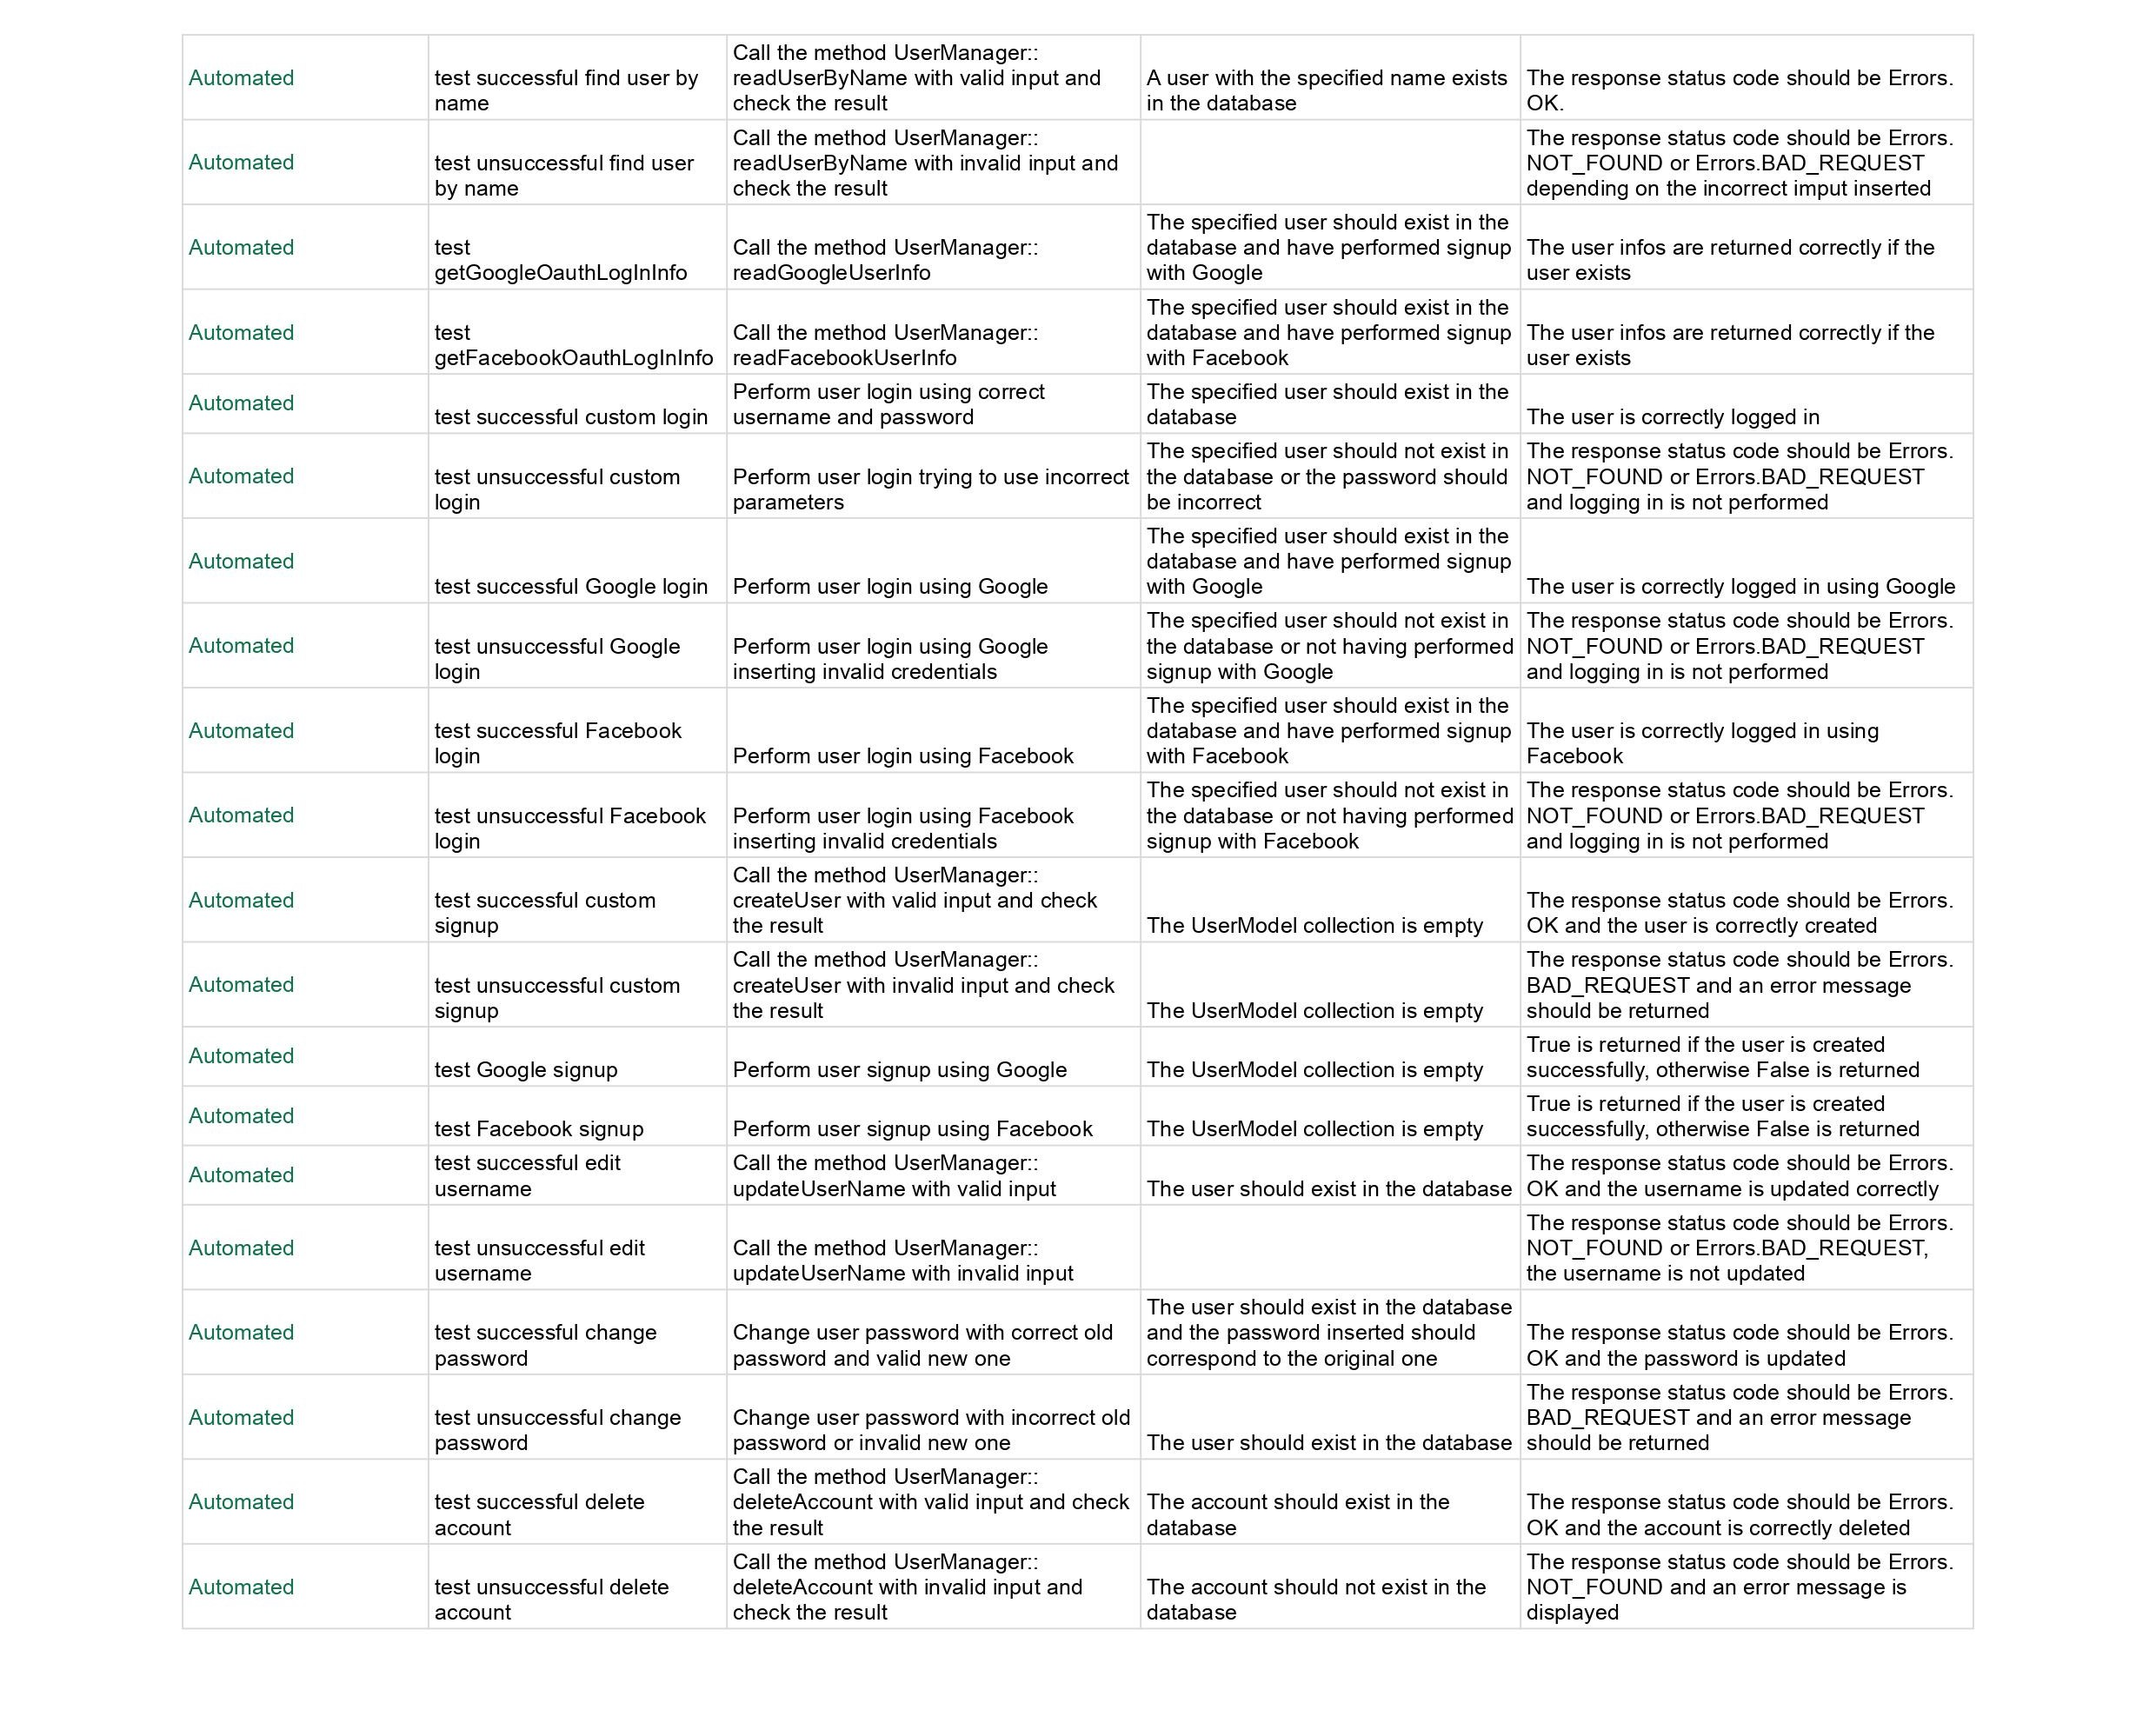
\includegraphics[width=0.95\textwidth]{images/Test_AccountManager.jpg}

\subsection*{Test DatabaseManager::UserManager}
This section is dedicated to the tests for the UserManager class, which is responsible for managing users in the database.
\newline
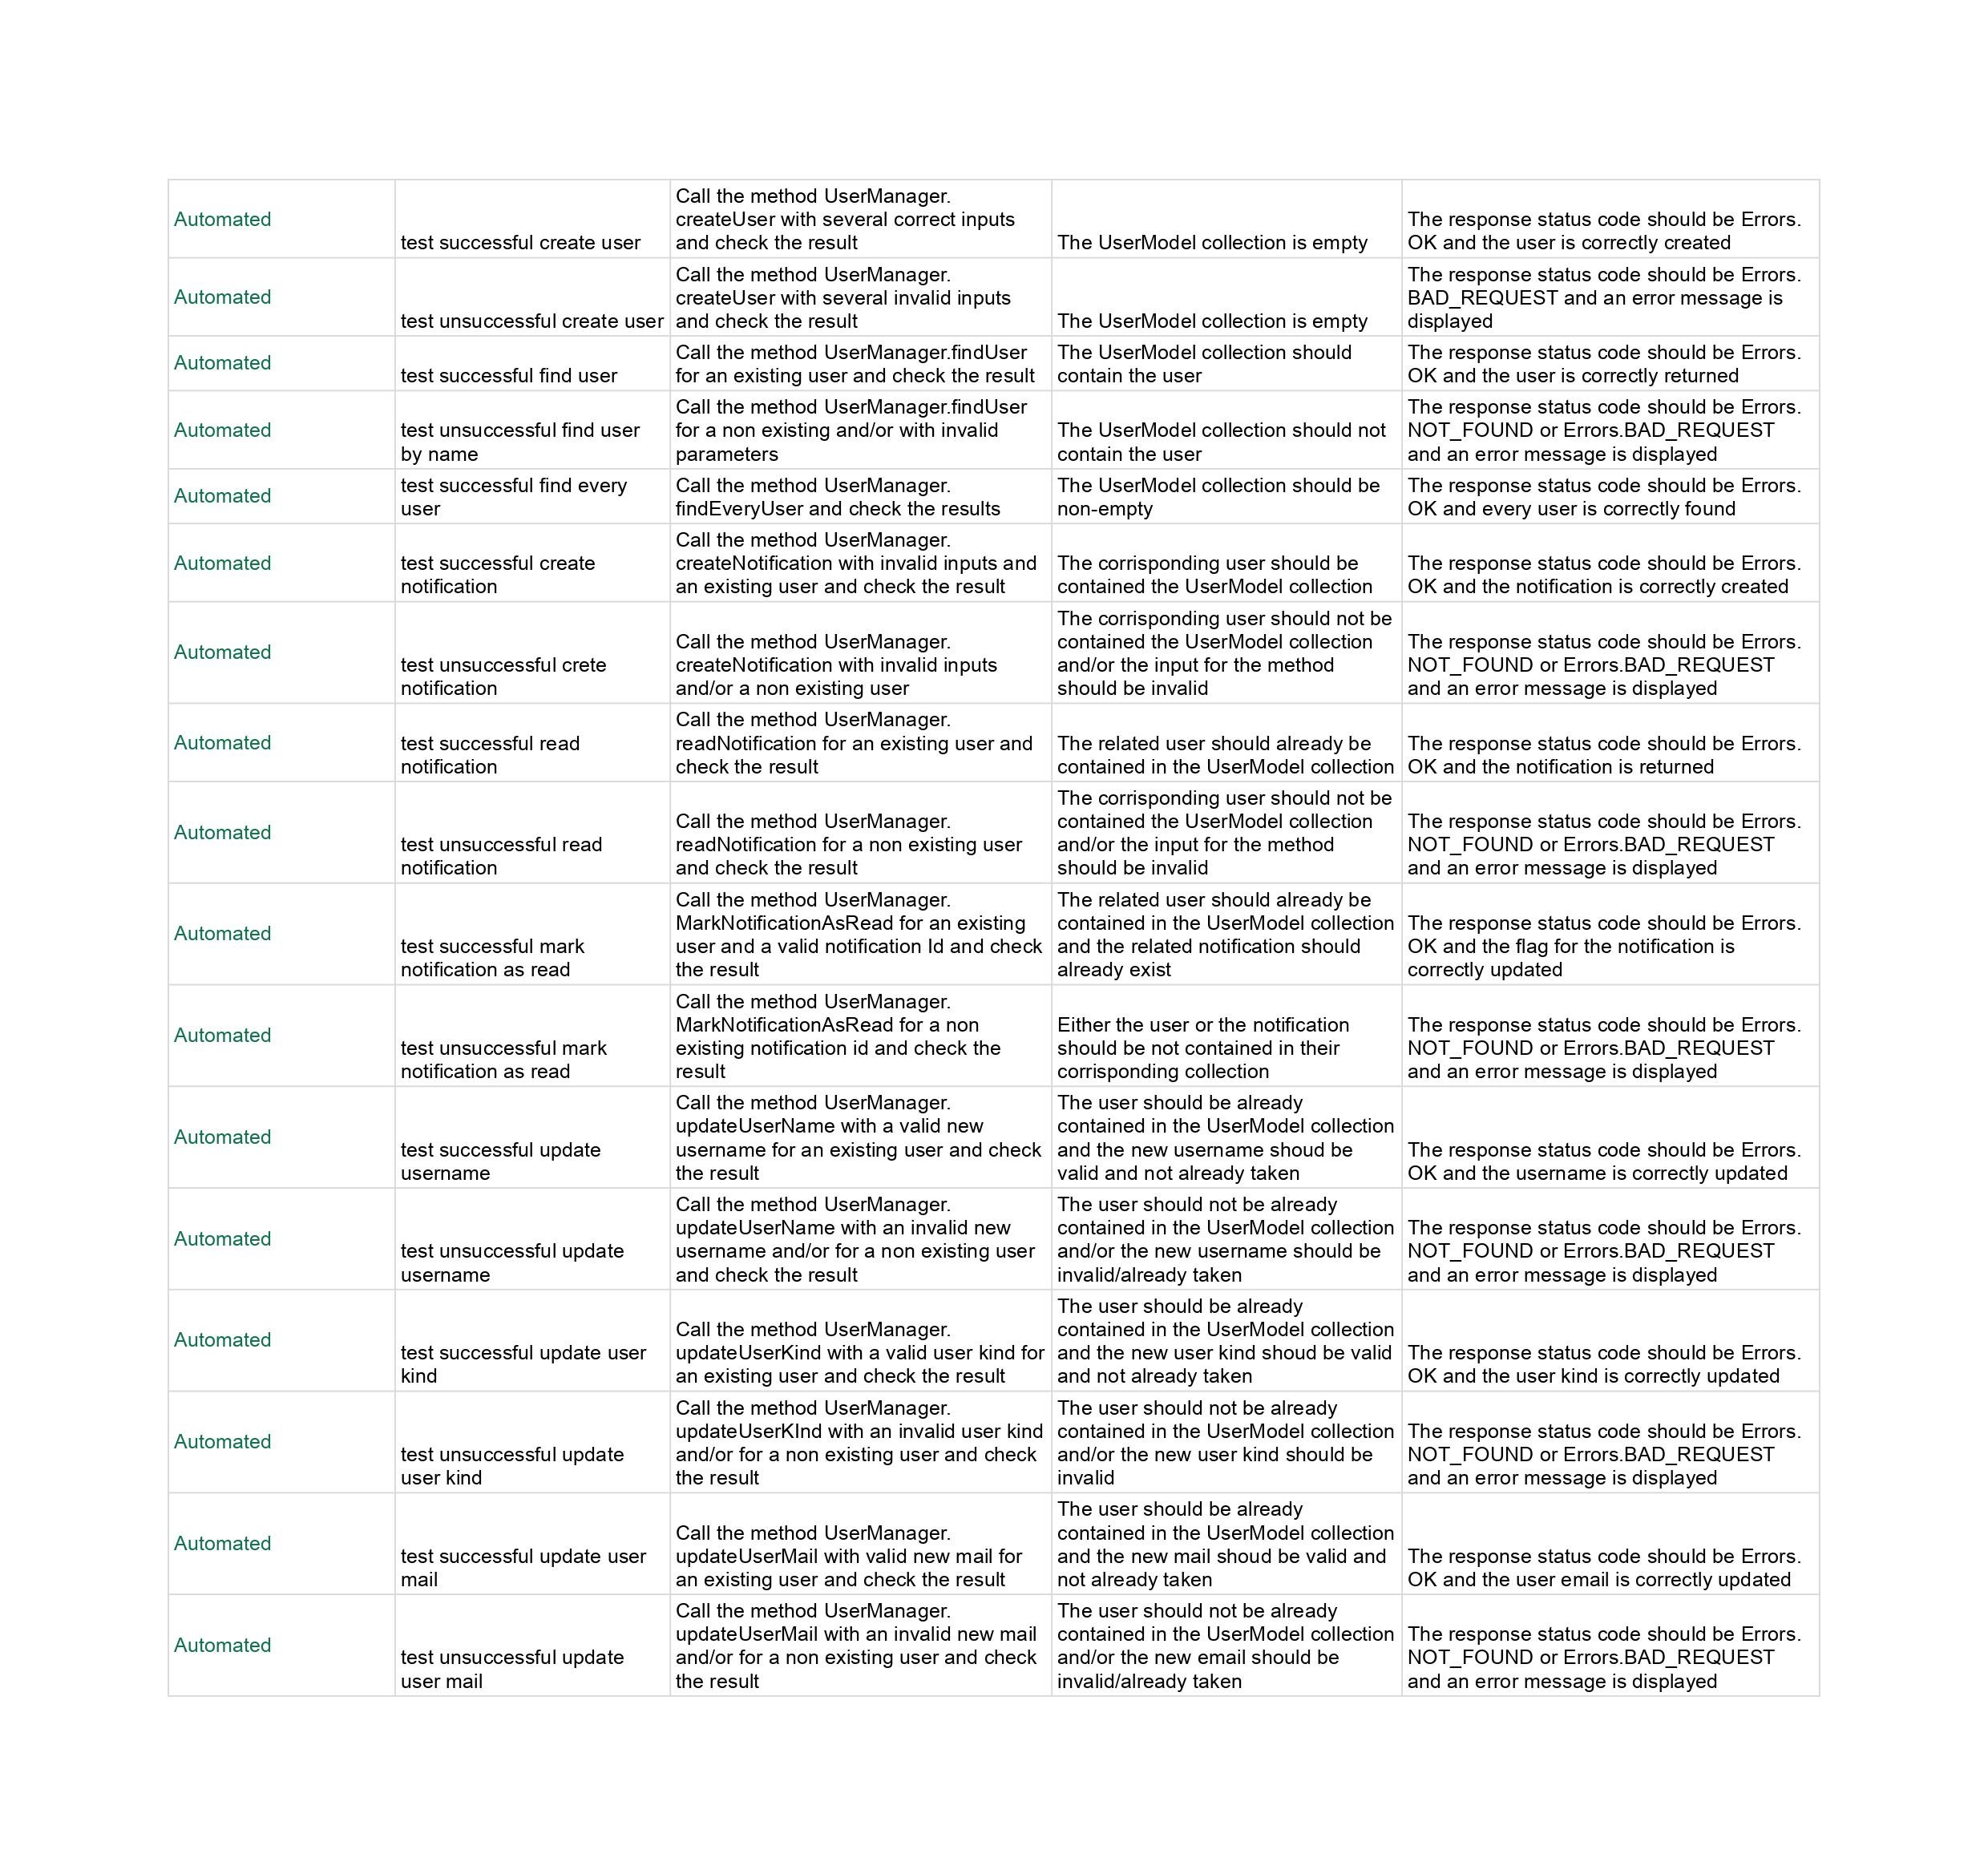
\includegraphics[width=0.95\textwidth]{images/Test_DatabaseManagerUserManager.jpg}

\subsection*{Test TaskManager}
This section includes automated tests for the TaskManager class, which is responsible for managing tasks in the database.
\newline
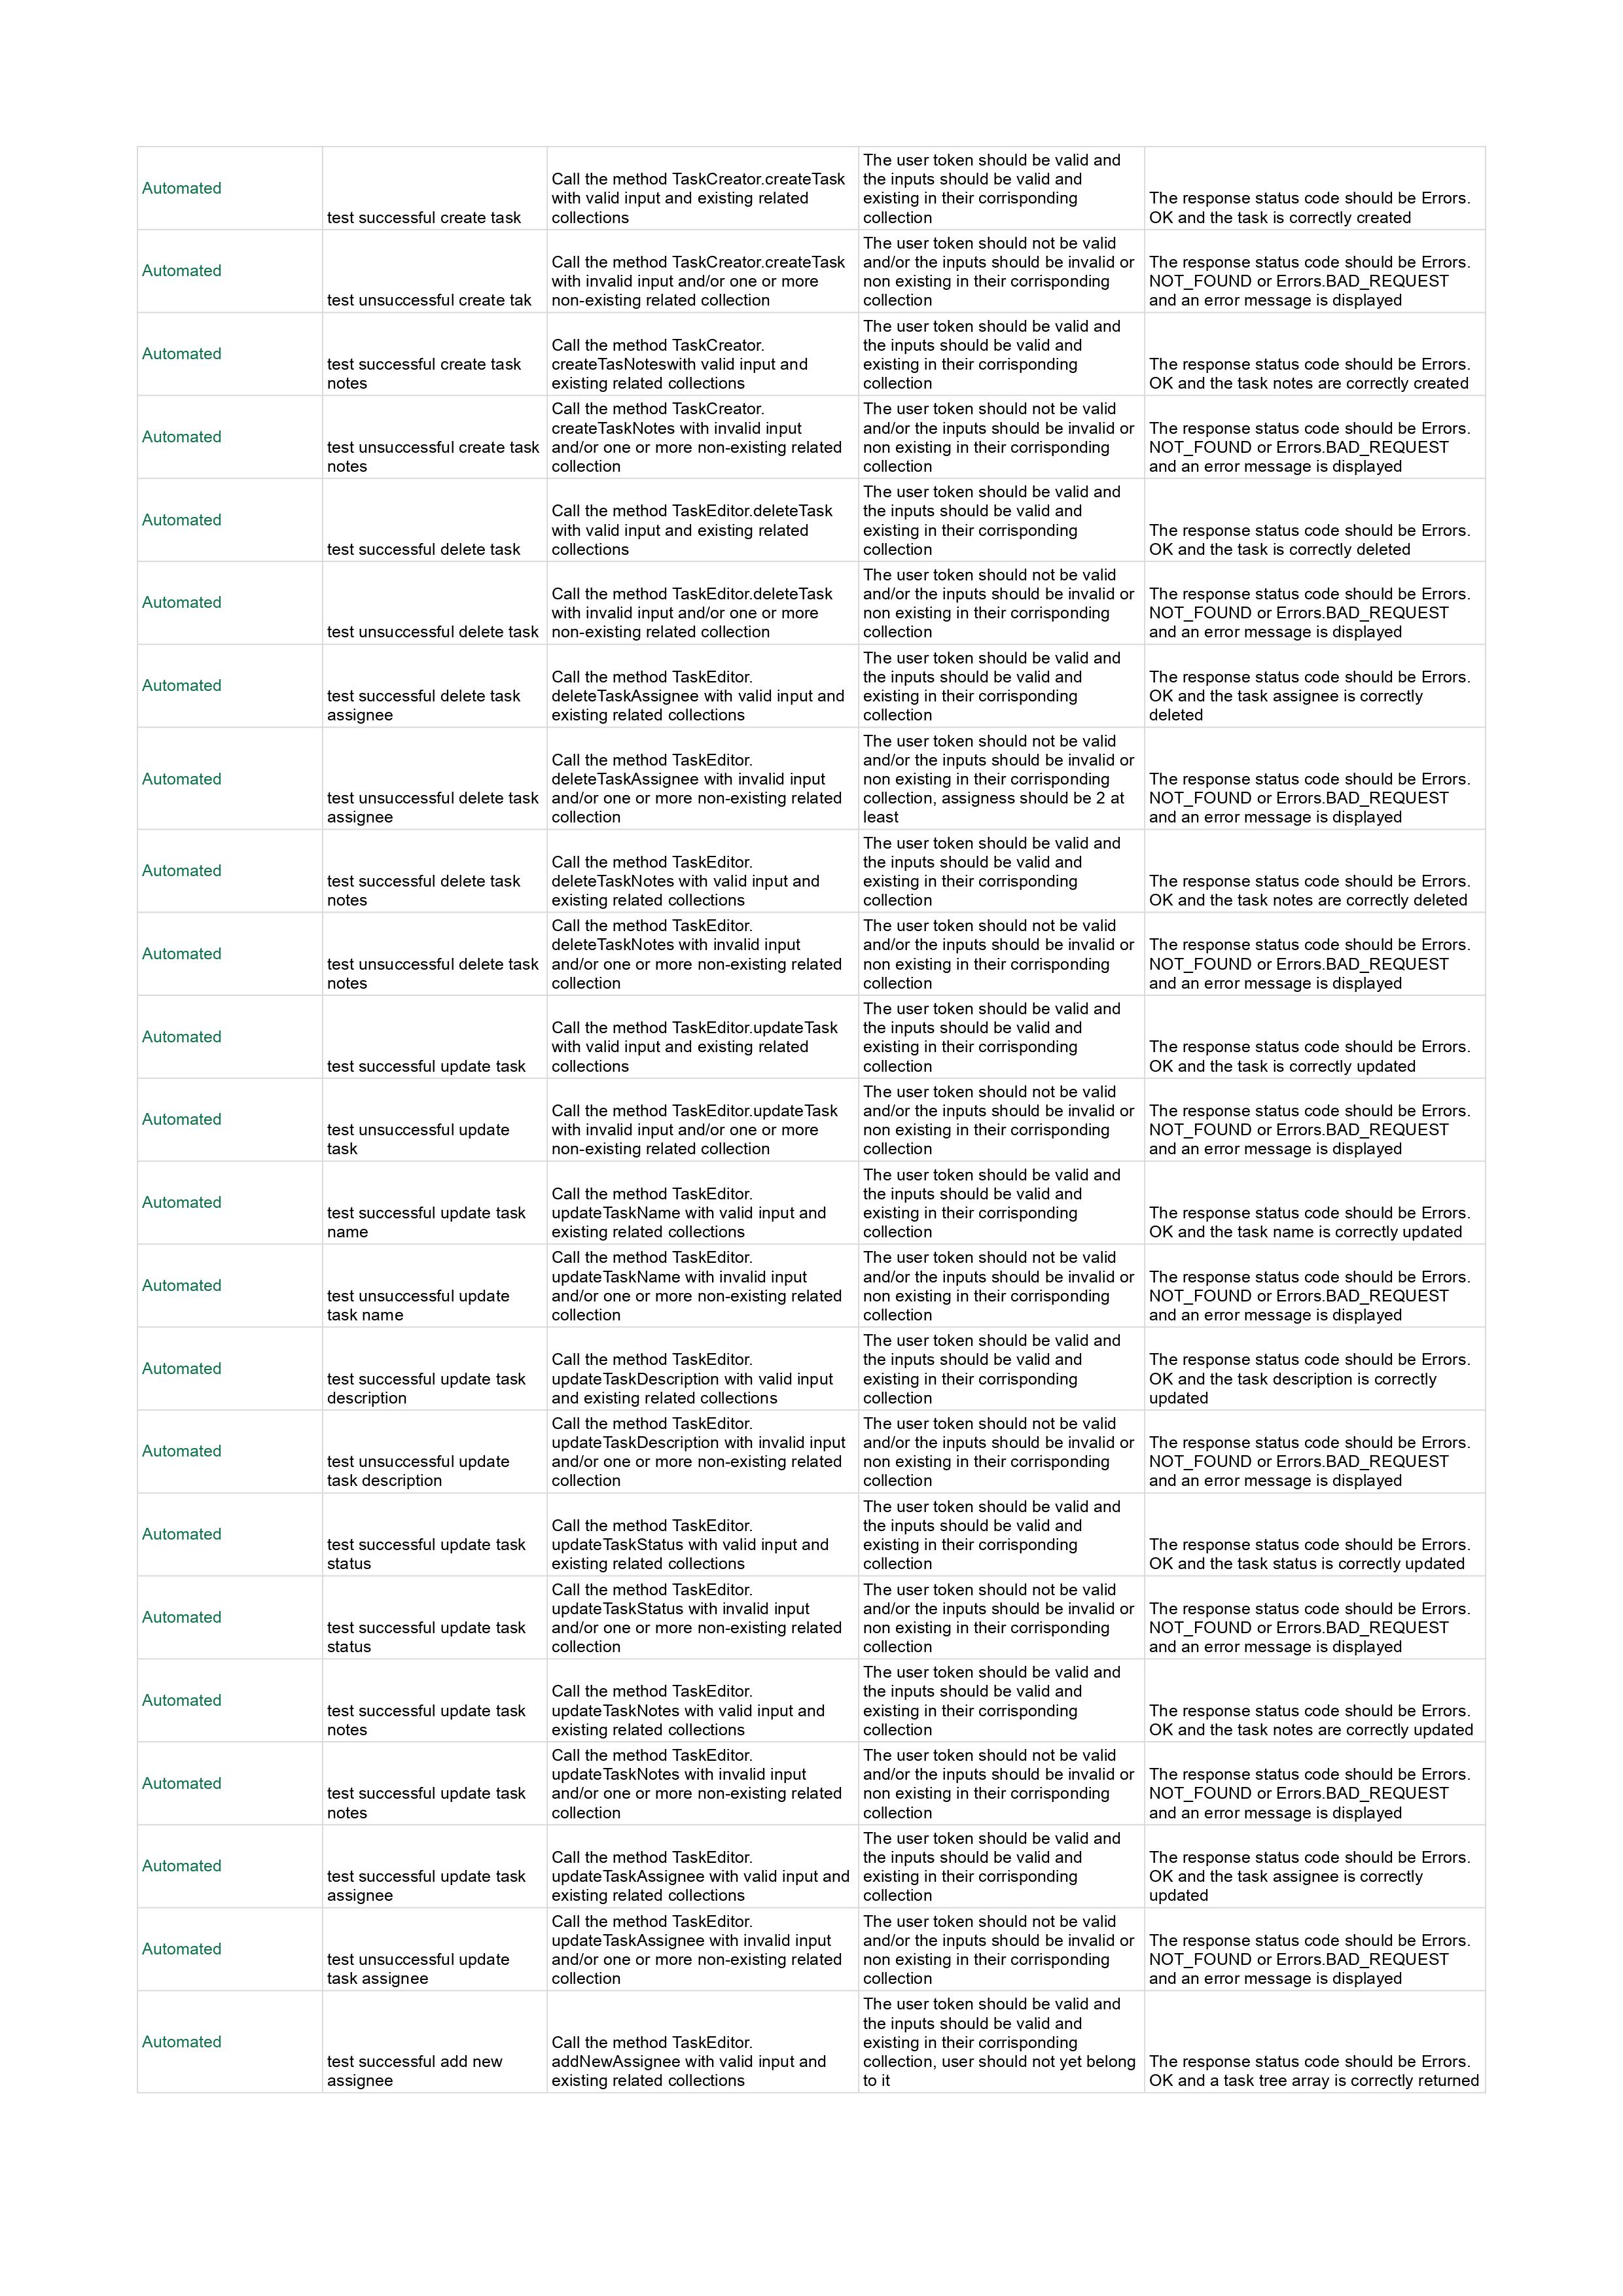
\includegraphics[width=0.95\textwidth]{images/Test_TaskManager-immagini-0.jpg}
\newline
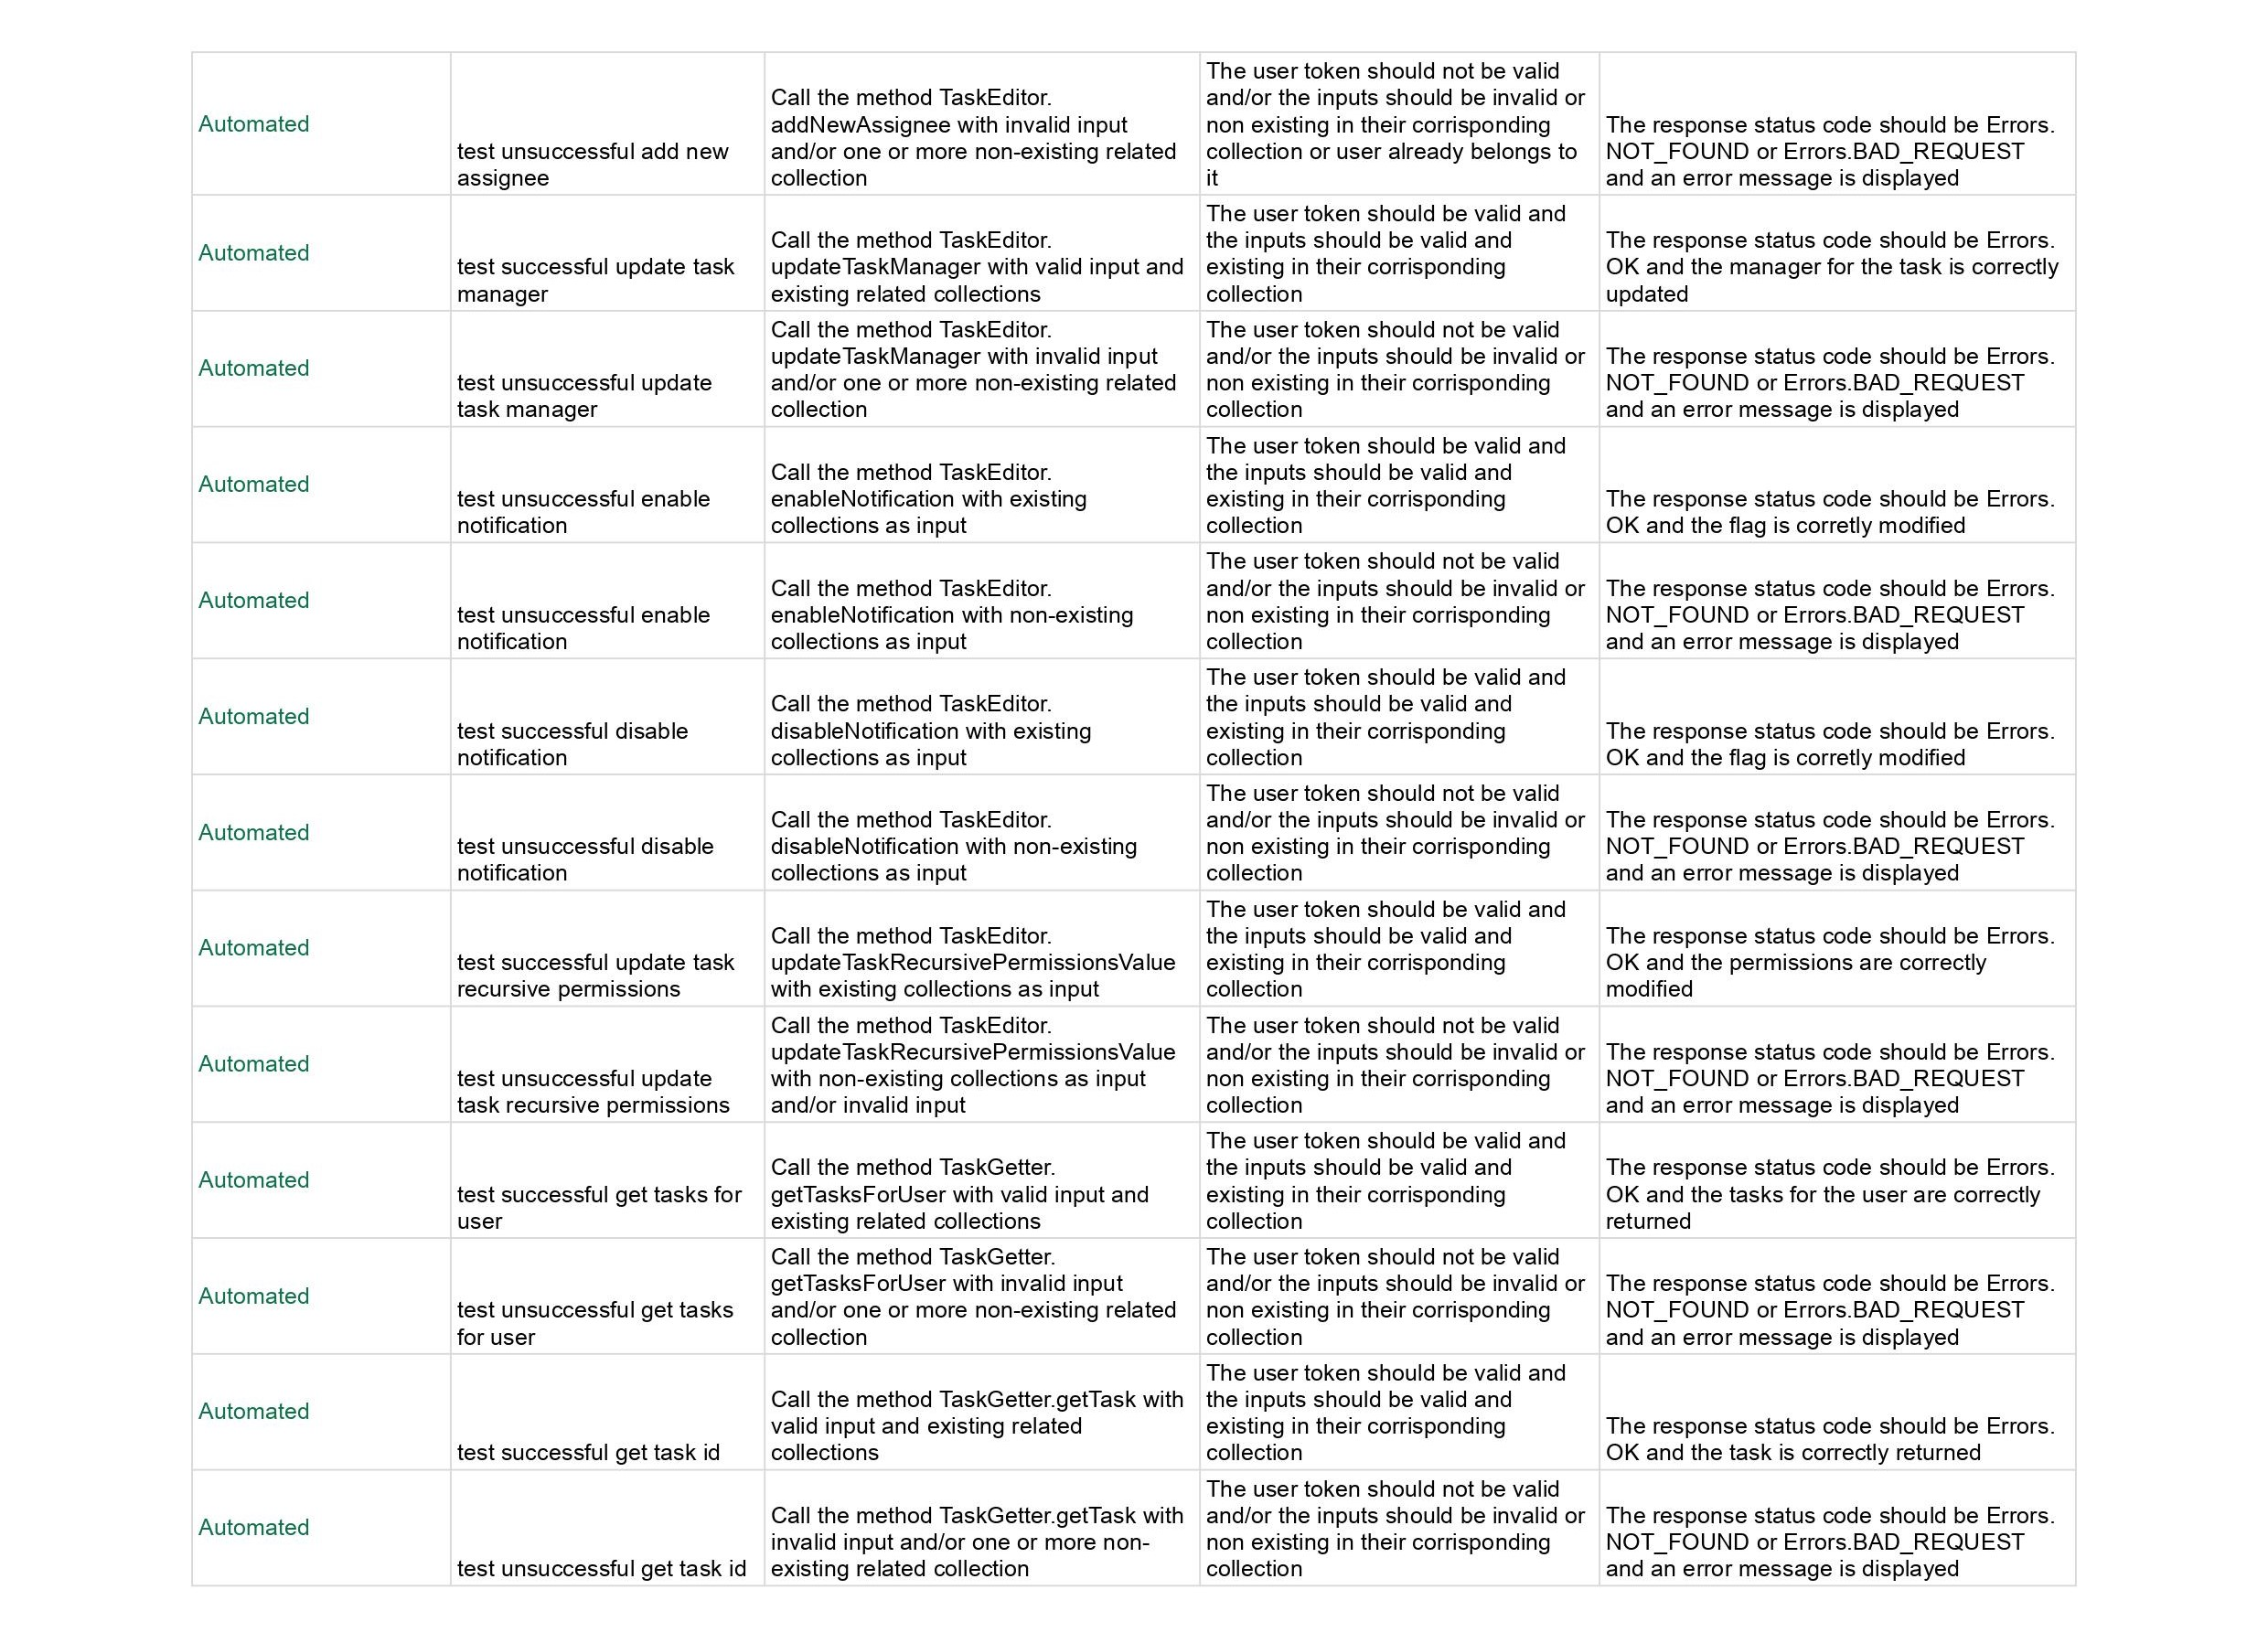
\includegraphics[width=0.95\textwidth]{images/Test_TaskManager-immagini-1.jpg}

\subsection*{Test Home Page}
This section includes manual tests for the home page.
\newline
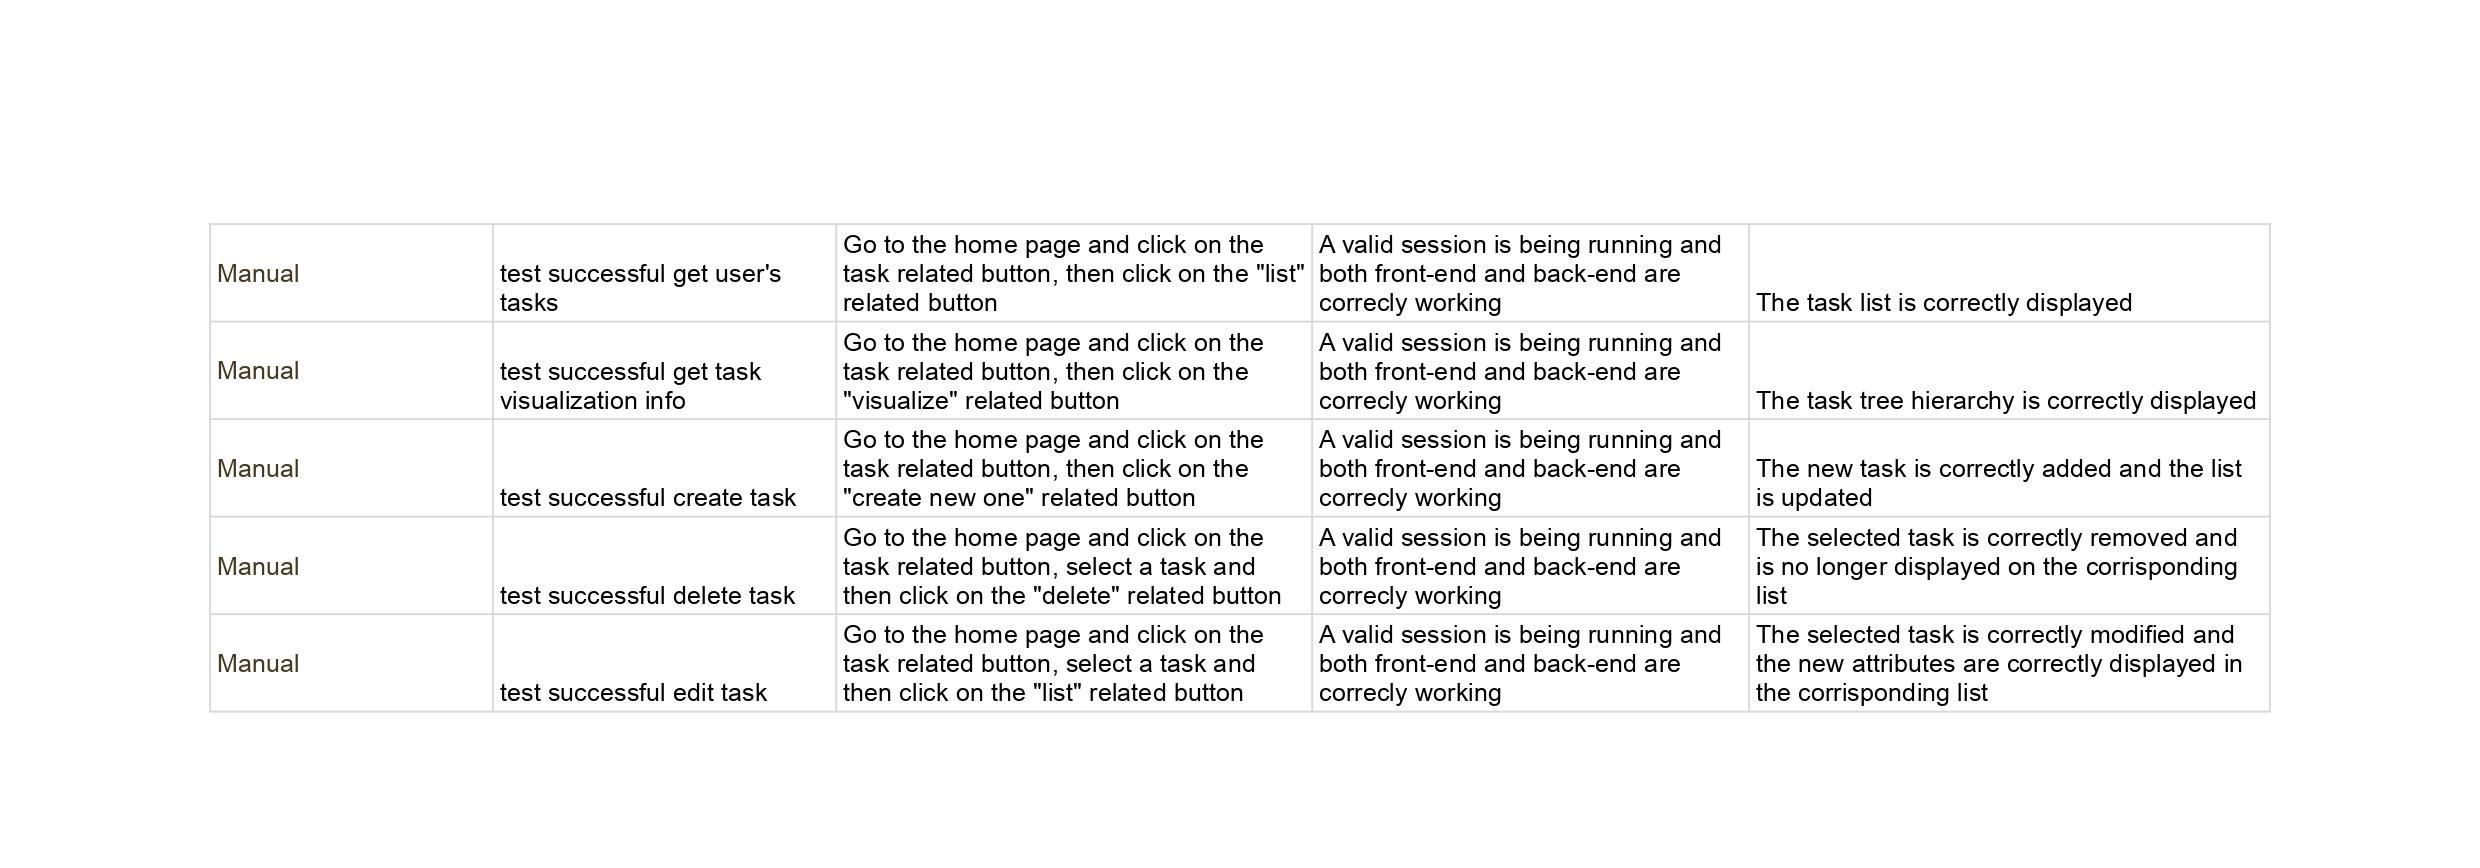
\includegraphics[width=0.95\textwidth]{images/Test_HomePage.jpg}

\subsection*{Test Notification View}
This section includes manual tests for the notification view.
\newline
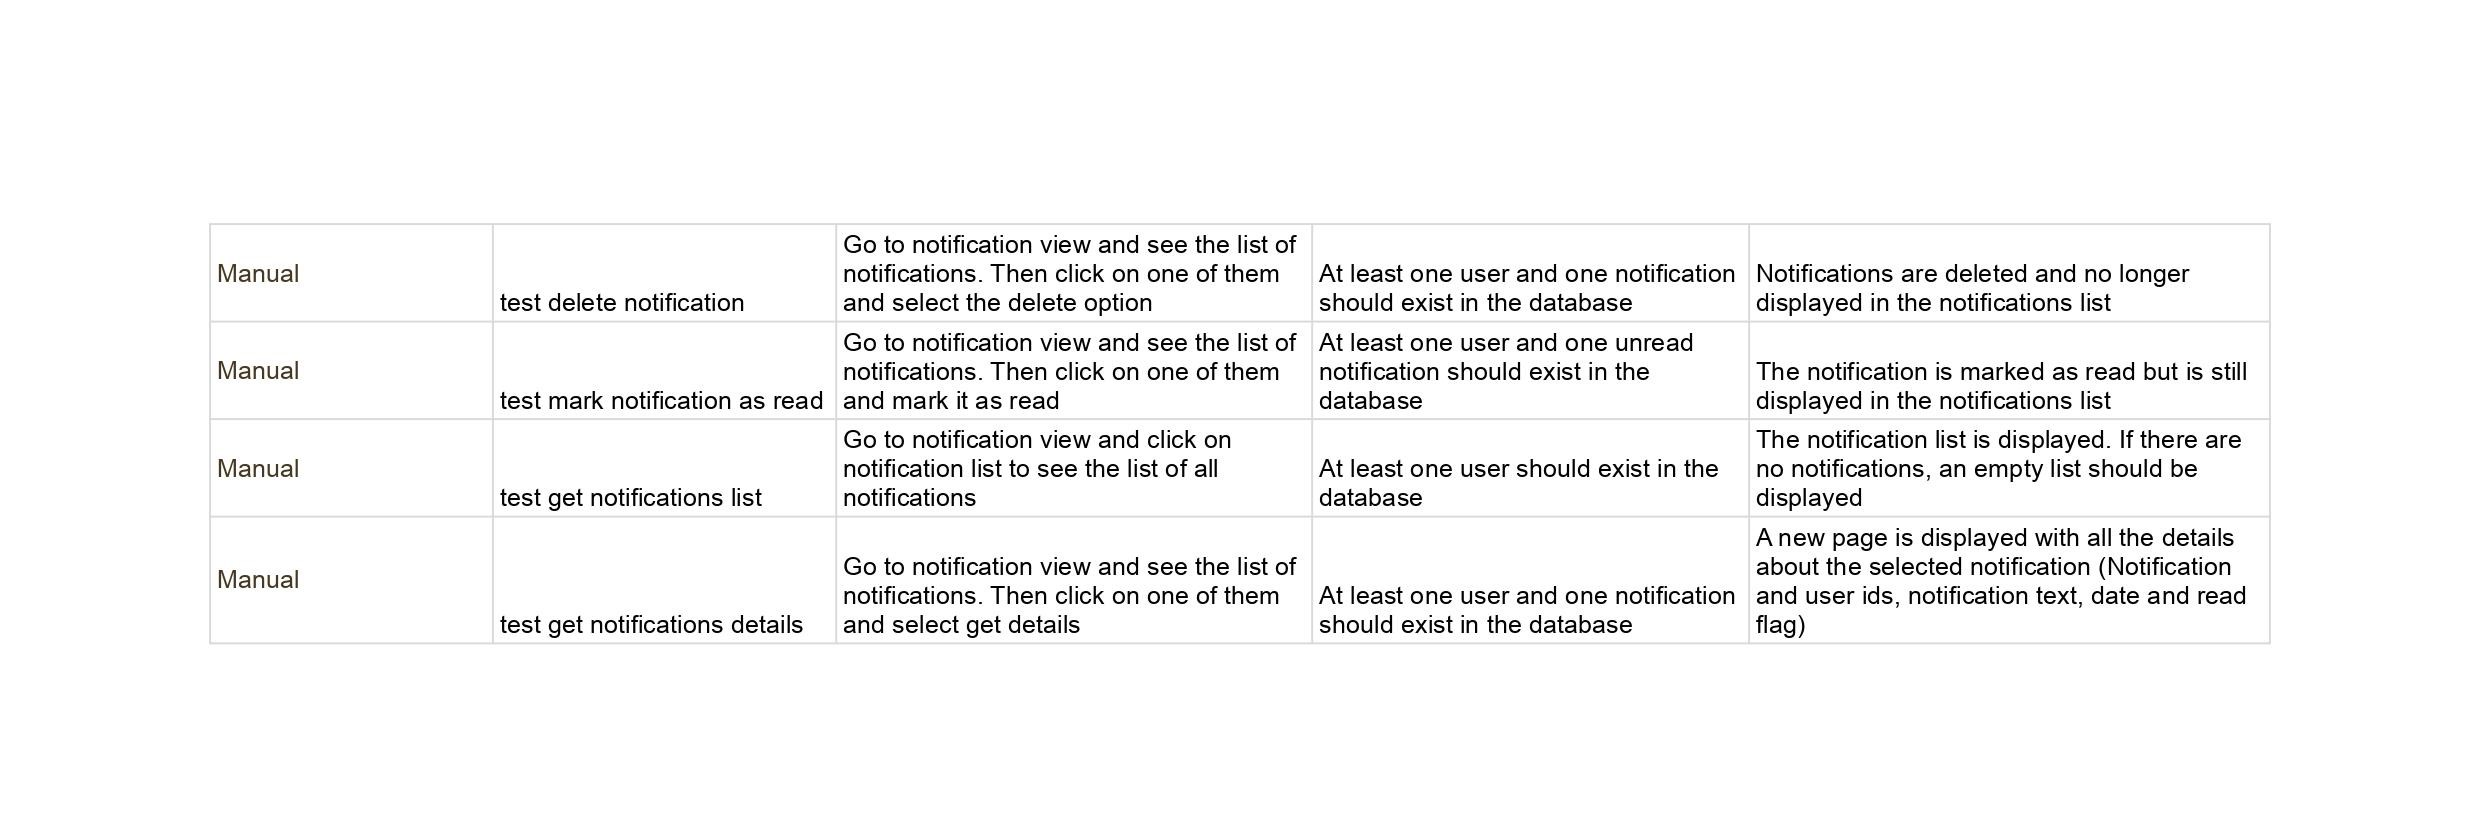
\includegraphics[width=0.95\textwidth]{images/Test_NotificationView.jpg}

\subsection*{Test Sign In and Sign Up Pages}
This section includes manual tests for the sign in and sign up pages.
\newline
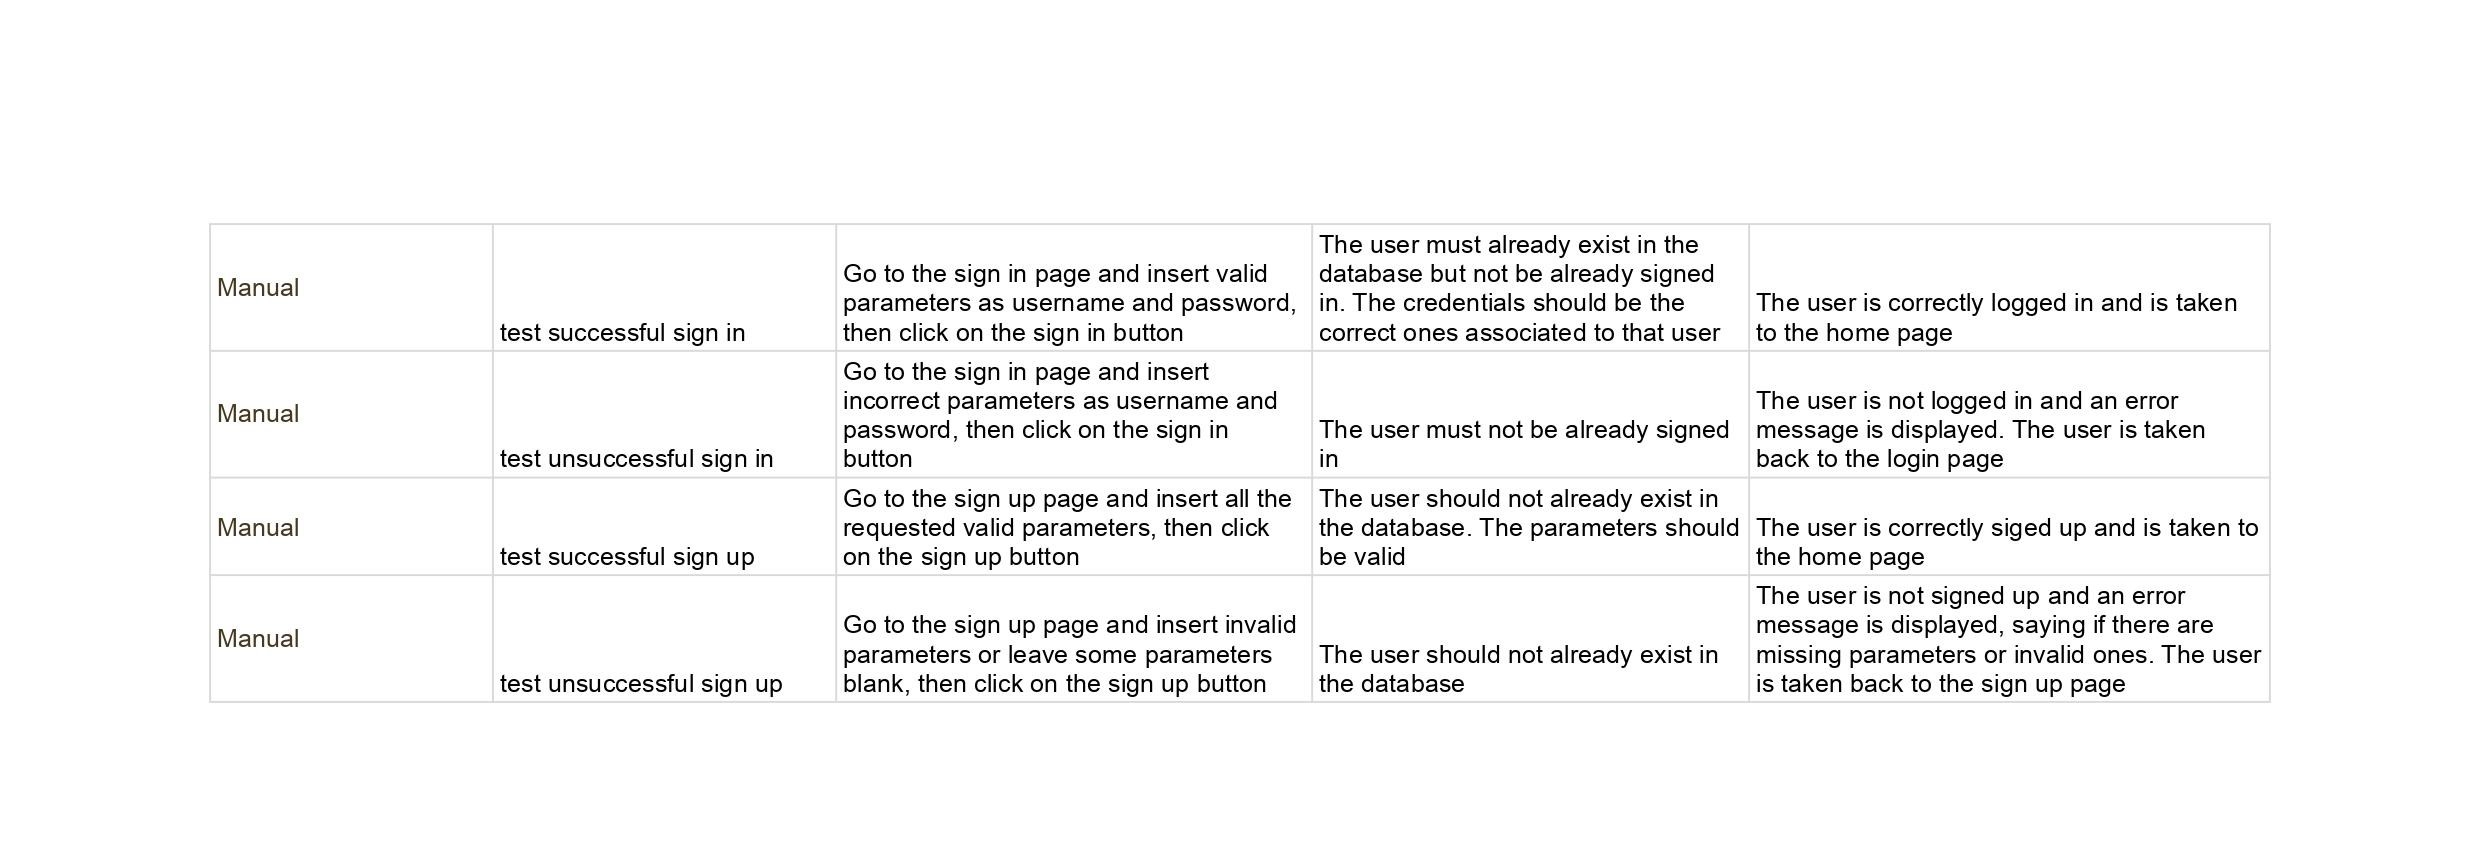
\includegraphics[width=0.95\textwidth]{images/Test_SignInSignUpPage.jpg}

\subsection*{Test Edit Profile Page}
This section includes manual tests for the edit profile page.
\newline
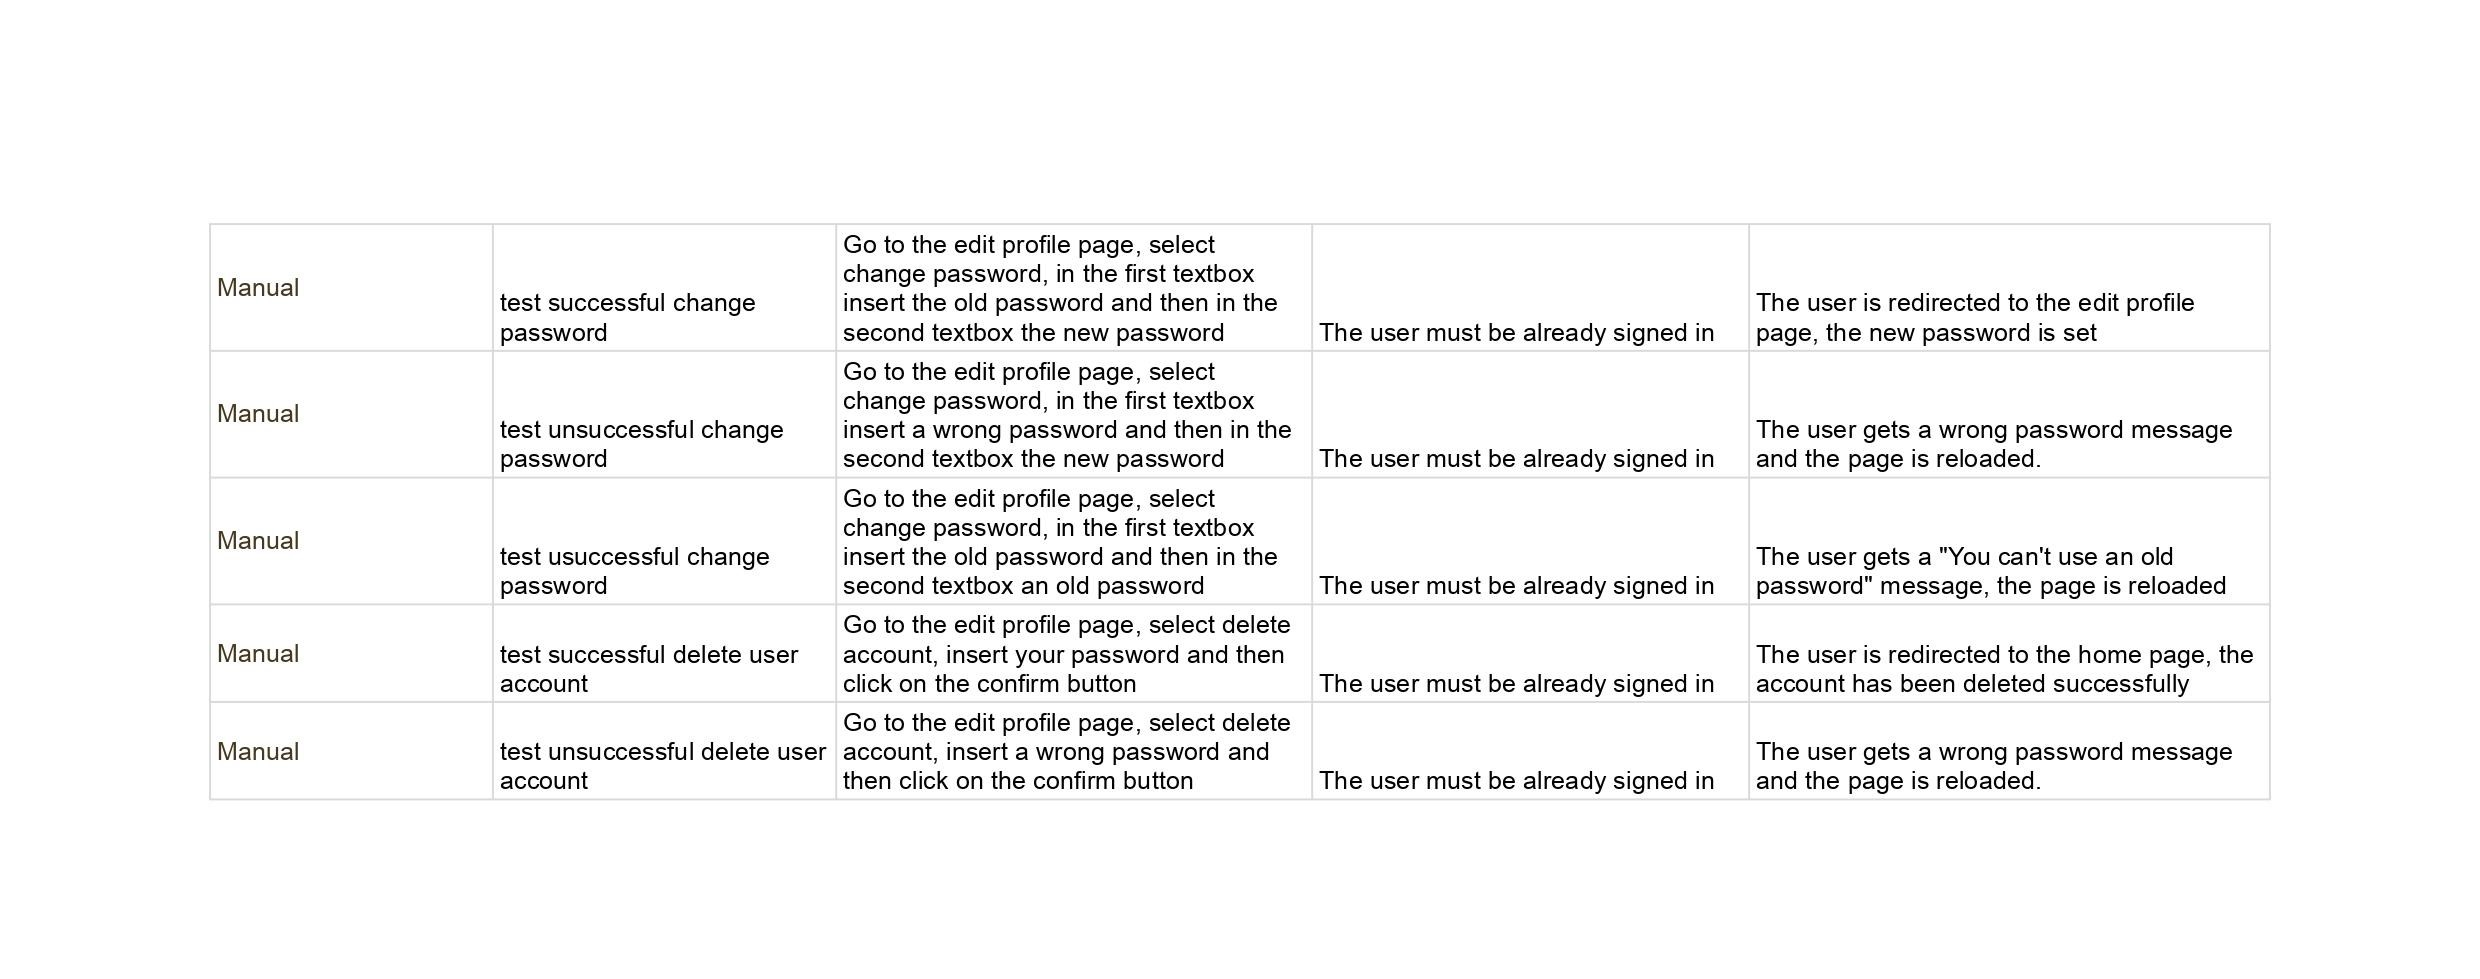
\includegraphics[width=0.95\textwidth]{images/Test_EditProfile.jpg}

\subsection*{Test Organization View Page}
This section includes manual tests for the organization view page.
\newline
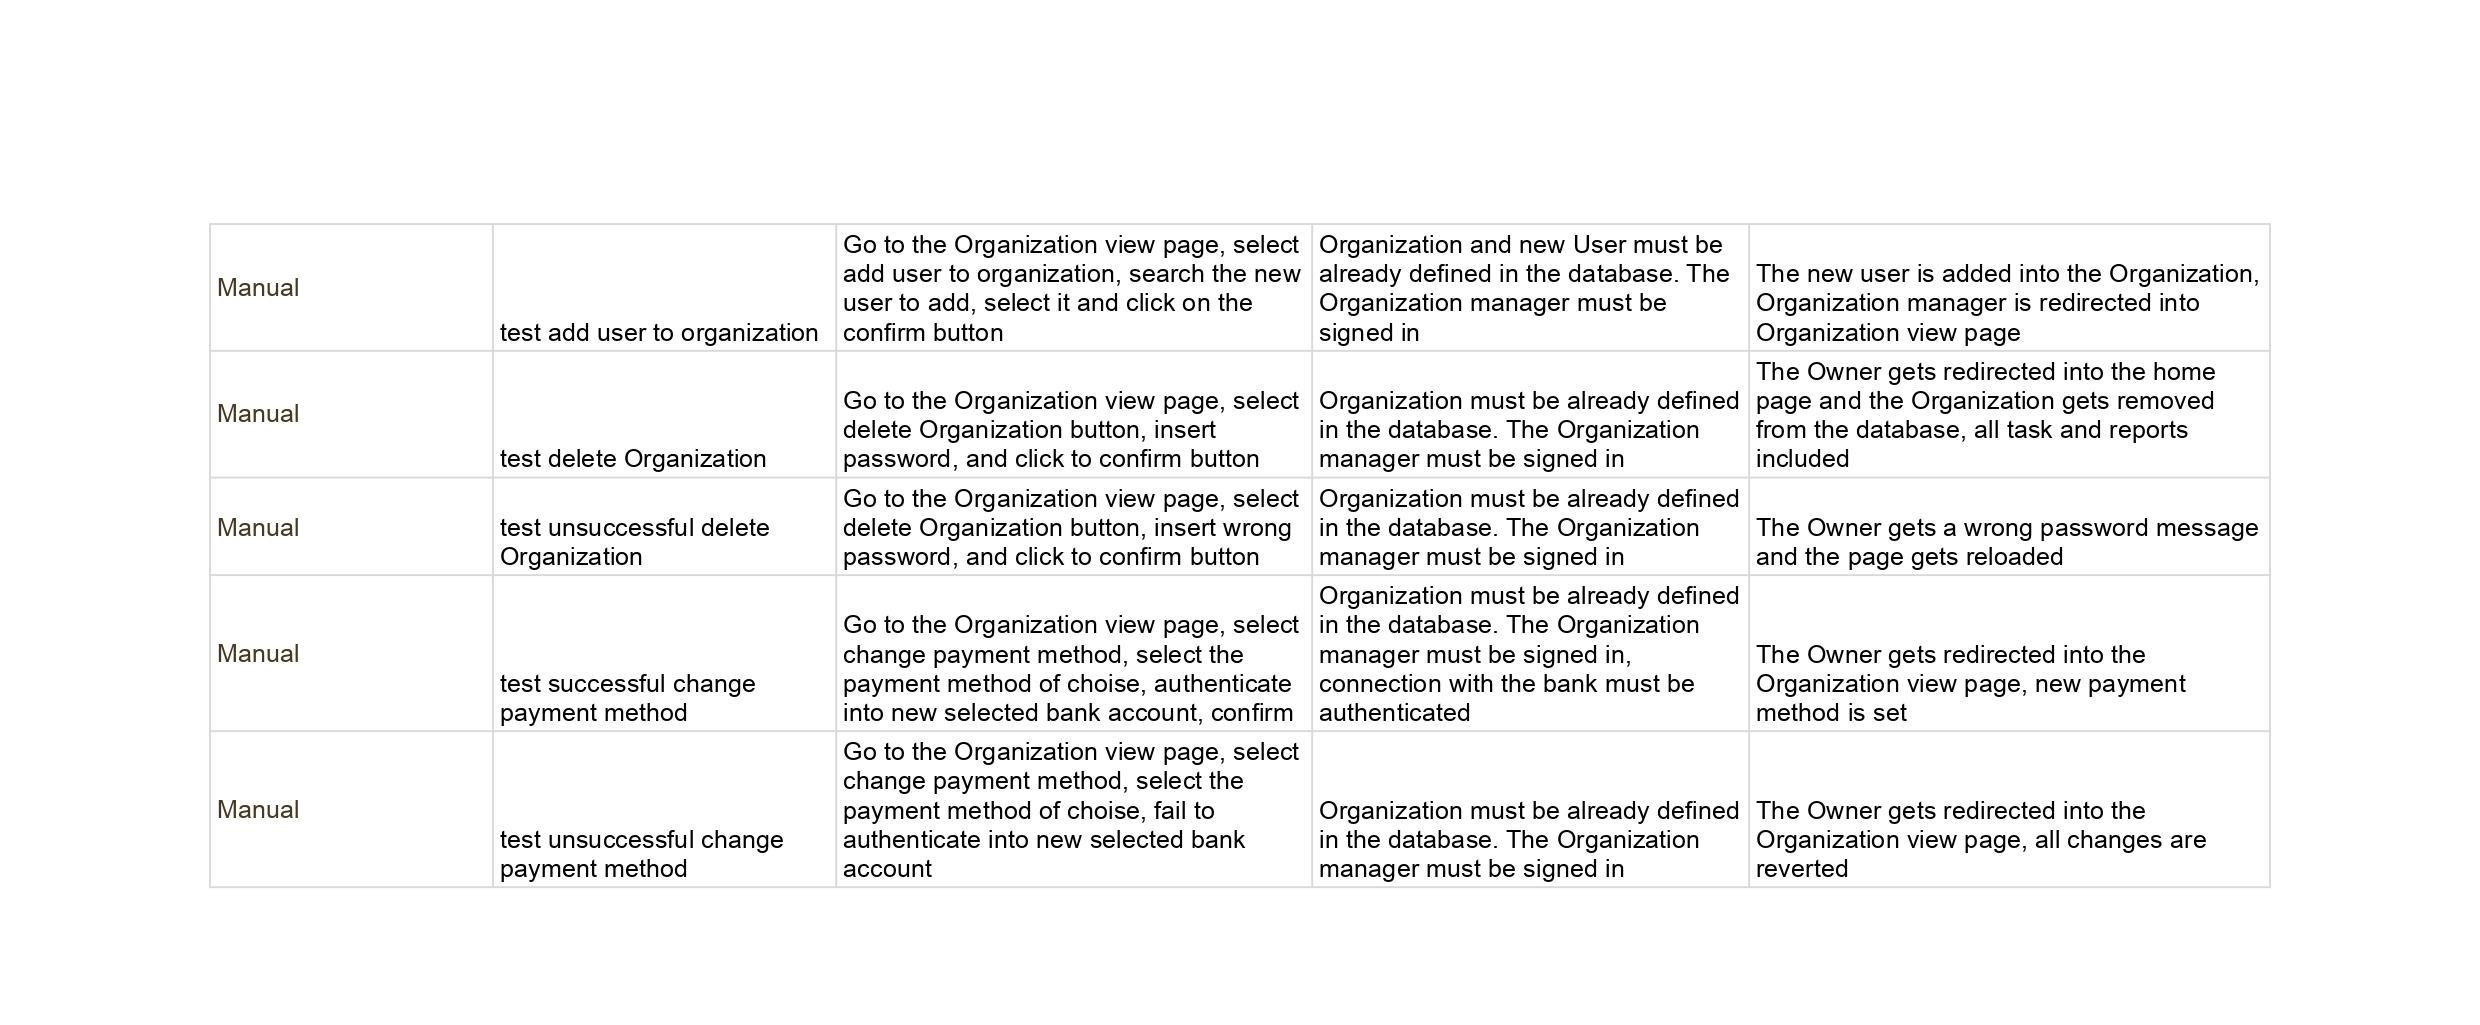
\includegraphics[width=0.95\textwidth]{images/Test_OrganizationView.jpg}

\section{Git Strategy}

Among the several git strategies available and commonly used, we have chosen \textbf{GitHub Flow}. We selected this strategy because it is \textit{one of the simplest} and is particularly suitable for \underline{small teams} like ours. GitHub Flow's straightforward approach, centered around a single branch with short-lived feature branches, allows us to maintain a \textbf{clean and manageable codebase}. This strategy also facilitates \textit{continuous integration and delivery}, making it easier to track progress and integrate changes seamlessly.



\section{Sprint 1}

\subsection{Backlog}
\includegraphics[width=0.95\textwidth]{images/sprint_backlog.jpg}

\subsection{Review and Retrospective}
\subsubsection{Retrospective}
Overall, the sprint was successful, as we managed to complete all the tasks on time.

We experienced some minor slowdowns due to our unfamiliarity with \textit{JavaScript} and \textit{MongoDB}, but we ultimately overcame these challenges. This sprint has been a valuable learning experience, highlighting areas where we can improve our technical skills.

In terms of task estimation, our decision to adopt a \textbf{conservative approach} proved to be beneficial. The higher estimates allowed us to allocate sufficient time to each task, reducing stress and enabling us to handle unforeseen issues effectively.

Team coordination was commendable, though there is room for improvement. The \underline{meticulous division of labor} contributed significantly to our success. Each member had a clear understanding of their responsibilities, which facilitated smoother collaboration and minimized overlapping efforts. However, we need to refine our task distribution further to optimize efficiency.

One notable area for improvement is our handling of \textbf{code integration}. Merging diverging branches proved to be time-consuming and occasionally disrupted our workflow. To address this, we should implement more frequent integration practices and establish clearer guidelines for branch management. This will help us avoid the pitfalls of merging conflicts and enhance our overall productivity.

Looking ahead to the upcoming sprint, we should focus on better organizing the workload across the team. By distributing tasks more evenly and ensuring that everyone is aligned with our coding standards and best practices, we can mitigate potential bottlenecks and maintain a steady progress rate.

Additionally, we should continue to invest time in learning and mastering the technologies we are using. This will not only boost our efficiency but also increase the quality of our product.

In conclusion, while this sprint has been a success, it also highlighted several areas for potential growth. By addressing these issues and building on our strengths, we can look forward to an even more productive standard for out team as a whole.

\subsubsection{Review}

Due to the subset of the chosen tasks we did't have too much to show to the ``Product Owner'' at the end of the sprint.
We shown the automatic deployment of the backend on render, and the frontend on GitHub Pages. We also shown the
automated tests to the backend functionalities.
Overall, the product Owner was satisfied with the results of the sprint, and didn't ask us to change anything.

\subsection{Burn-down Chart}
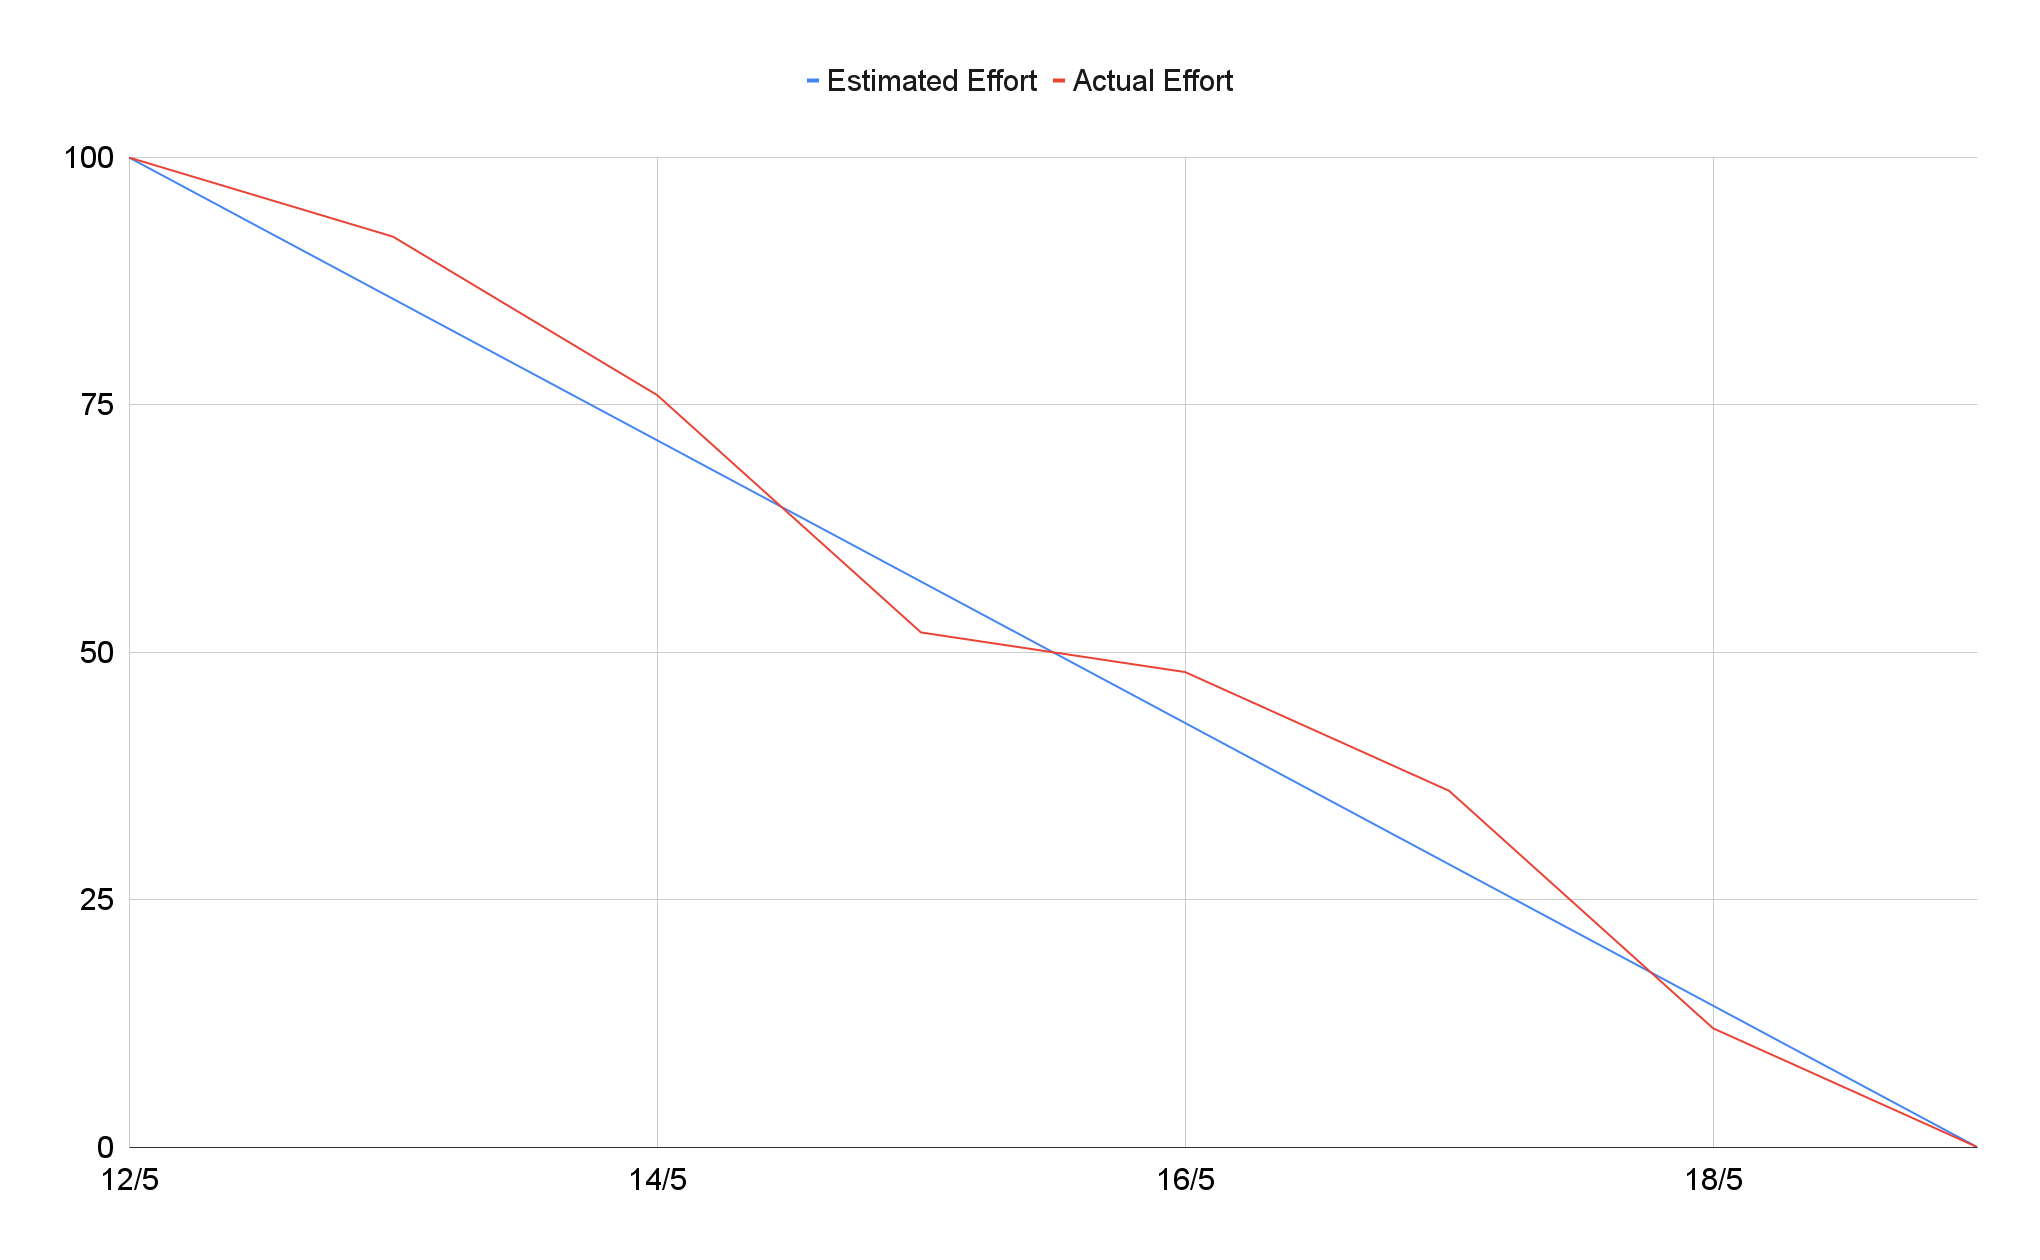
\includegraphics[width=0.95\textwidth]{images/burndown_chart.png}

\section{Sprint 2}

\subsection{Backlog}
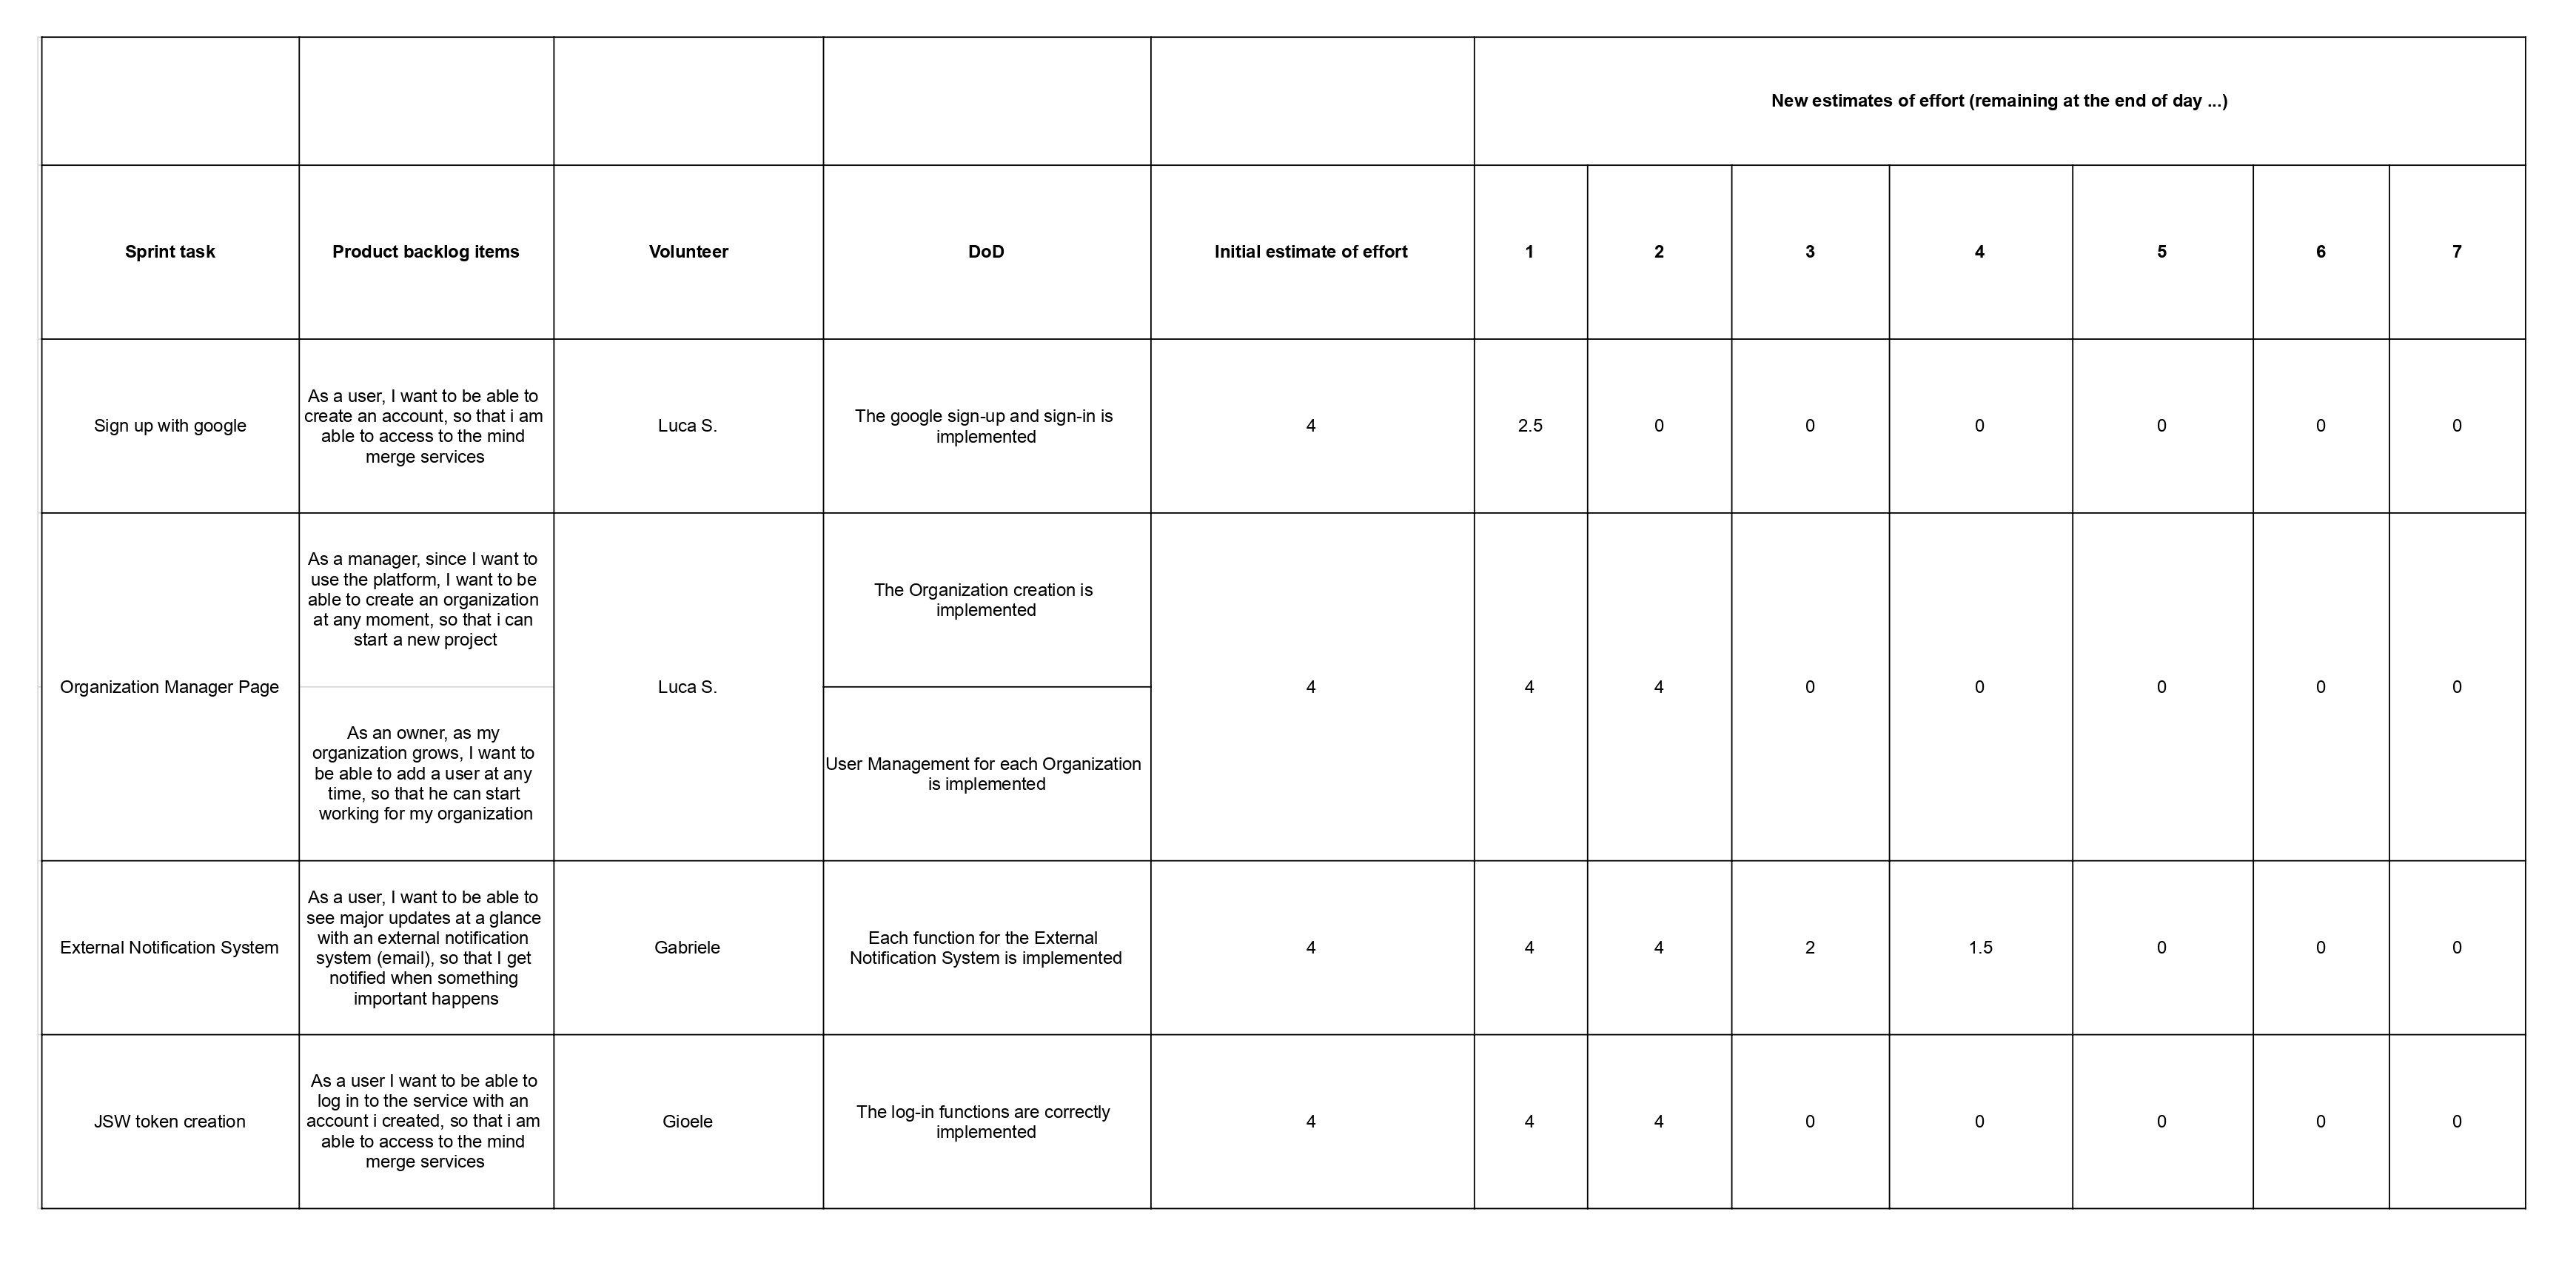
\includegraphics[width=0.95\textwidth]{images/sprint_backlog_2.jpg}

\subsection{Review and Retrospective}

\subsubsection{Retrospective}
Sprint 2 went well overall. However, as reflected in the burndown chart, we underestimated our velocity. This was primarily because we allocated a significant amount of time during the week for another course project that we anticipated would require considerable effort. To our surprise, we completed that project in one day, leaving us with more available time for the rest of the week.

Our main concern going into Sprint 3 is becoming more familiar with the Vue framework. By the end of Sprint 2, we still faced challenges in using it effectively.

\subsubsection{Review}
We demonstrated the Google sign-in functionality and the "Organization Manager" page to the product owner. This page allows users to create an organization and add or remove users.

The product owner was happy with the results but requested a change. Specifically, he asked that when a new organization is created, it should automatically be selected as the current active organization. We will note this down and address it in one of the upcoming sprints.
\subsection{Burn-down Chart}
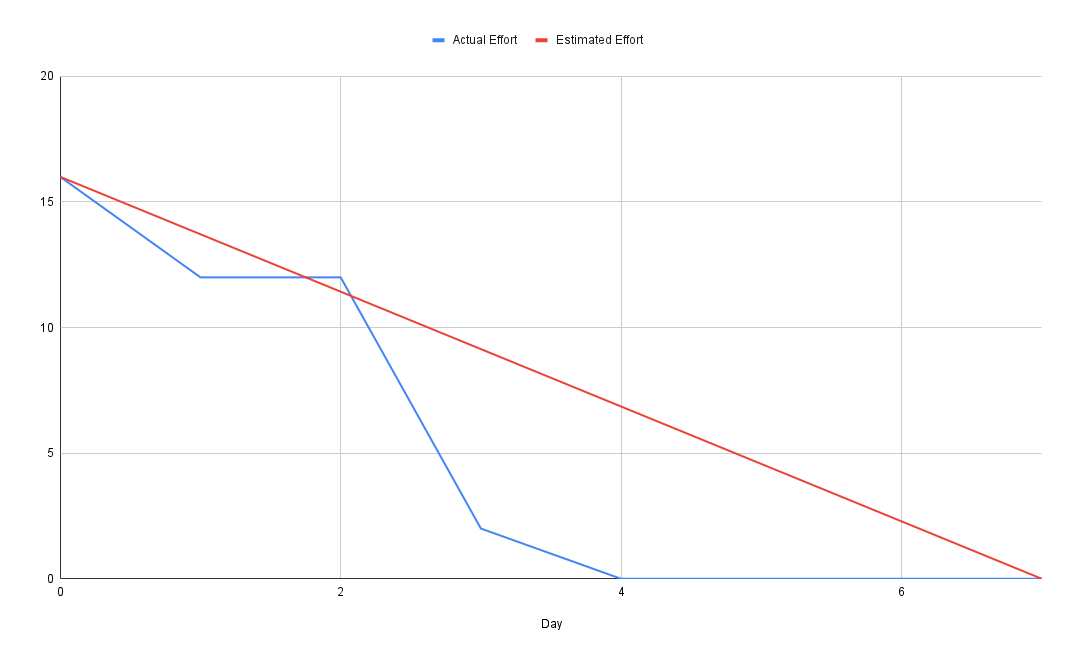
\includegraphics[width=0.95\textwidth]{images/burndown_chart_2.png}

\section{Sprint 3}

\subsection{Backlog}
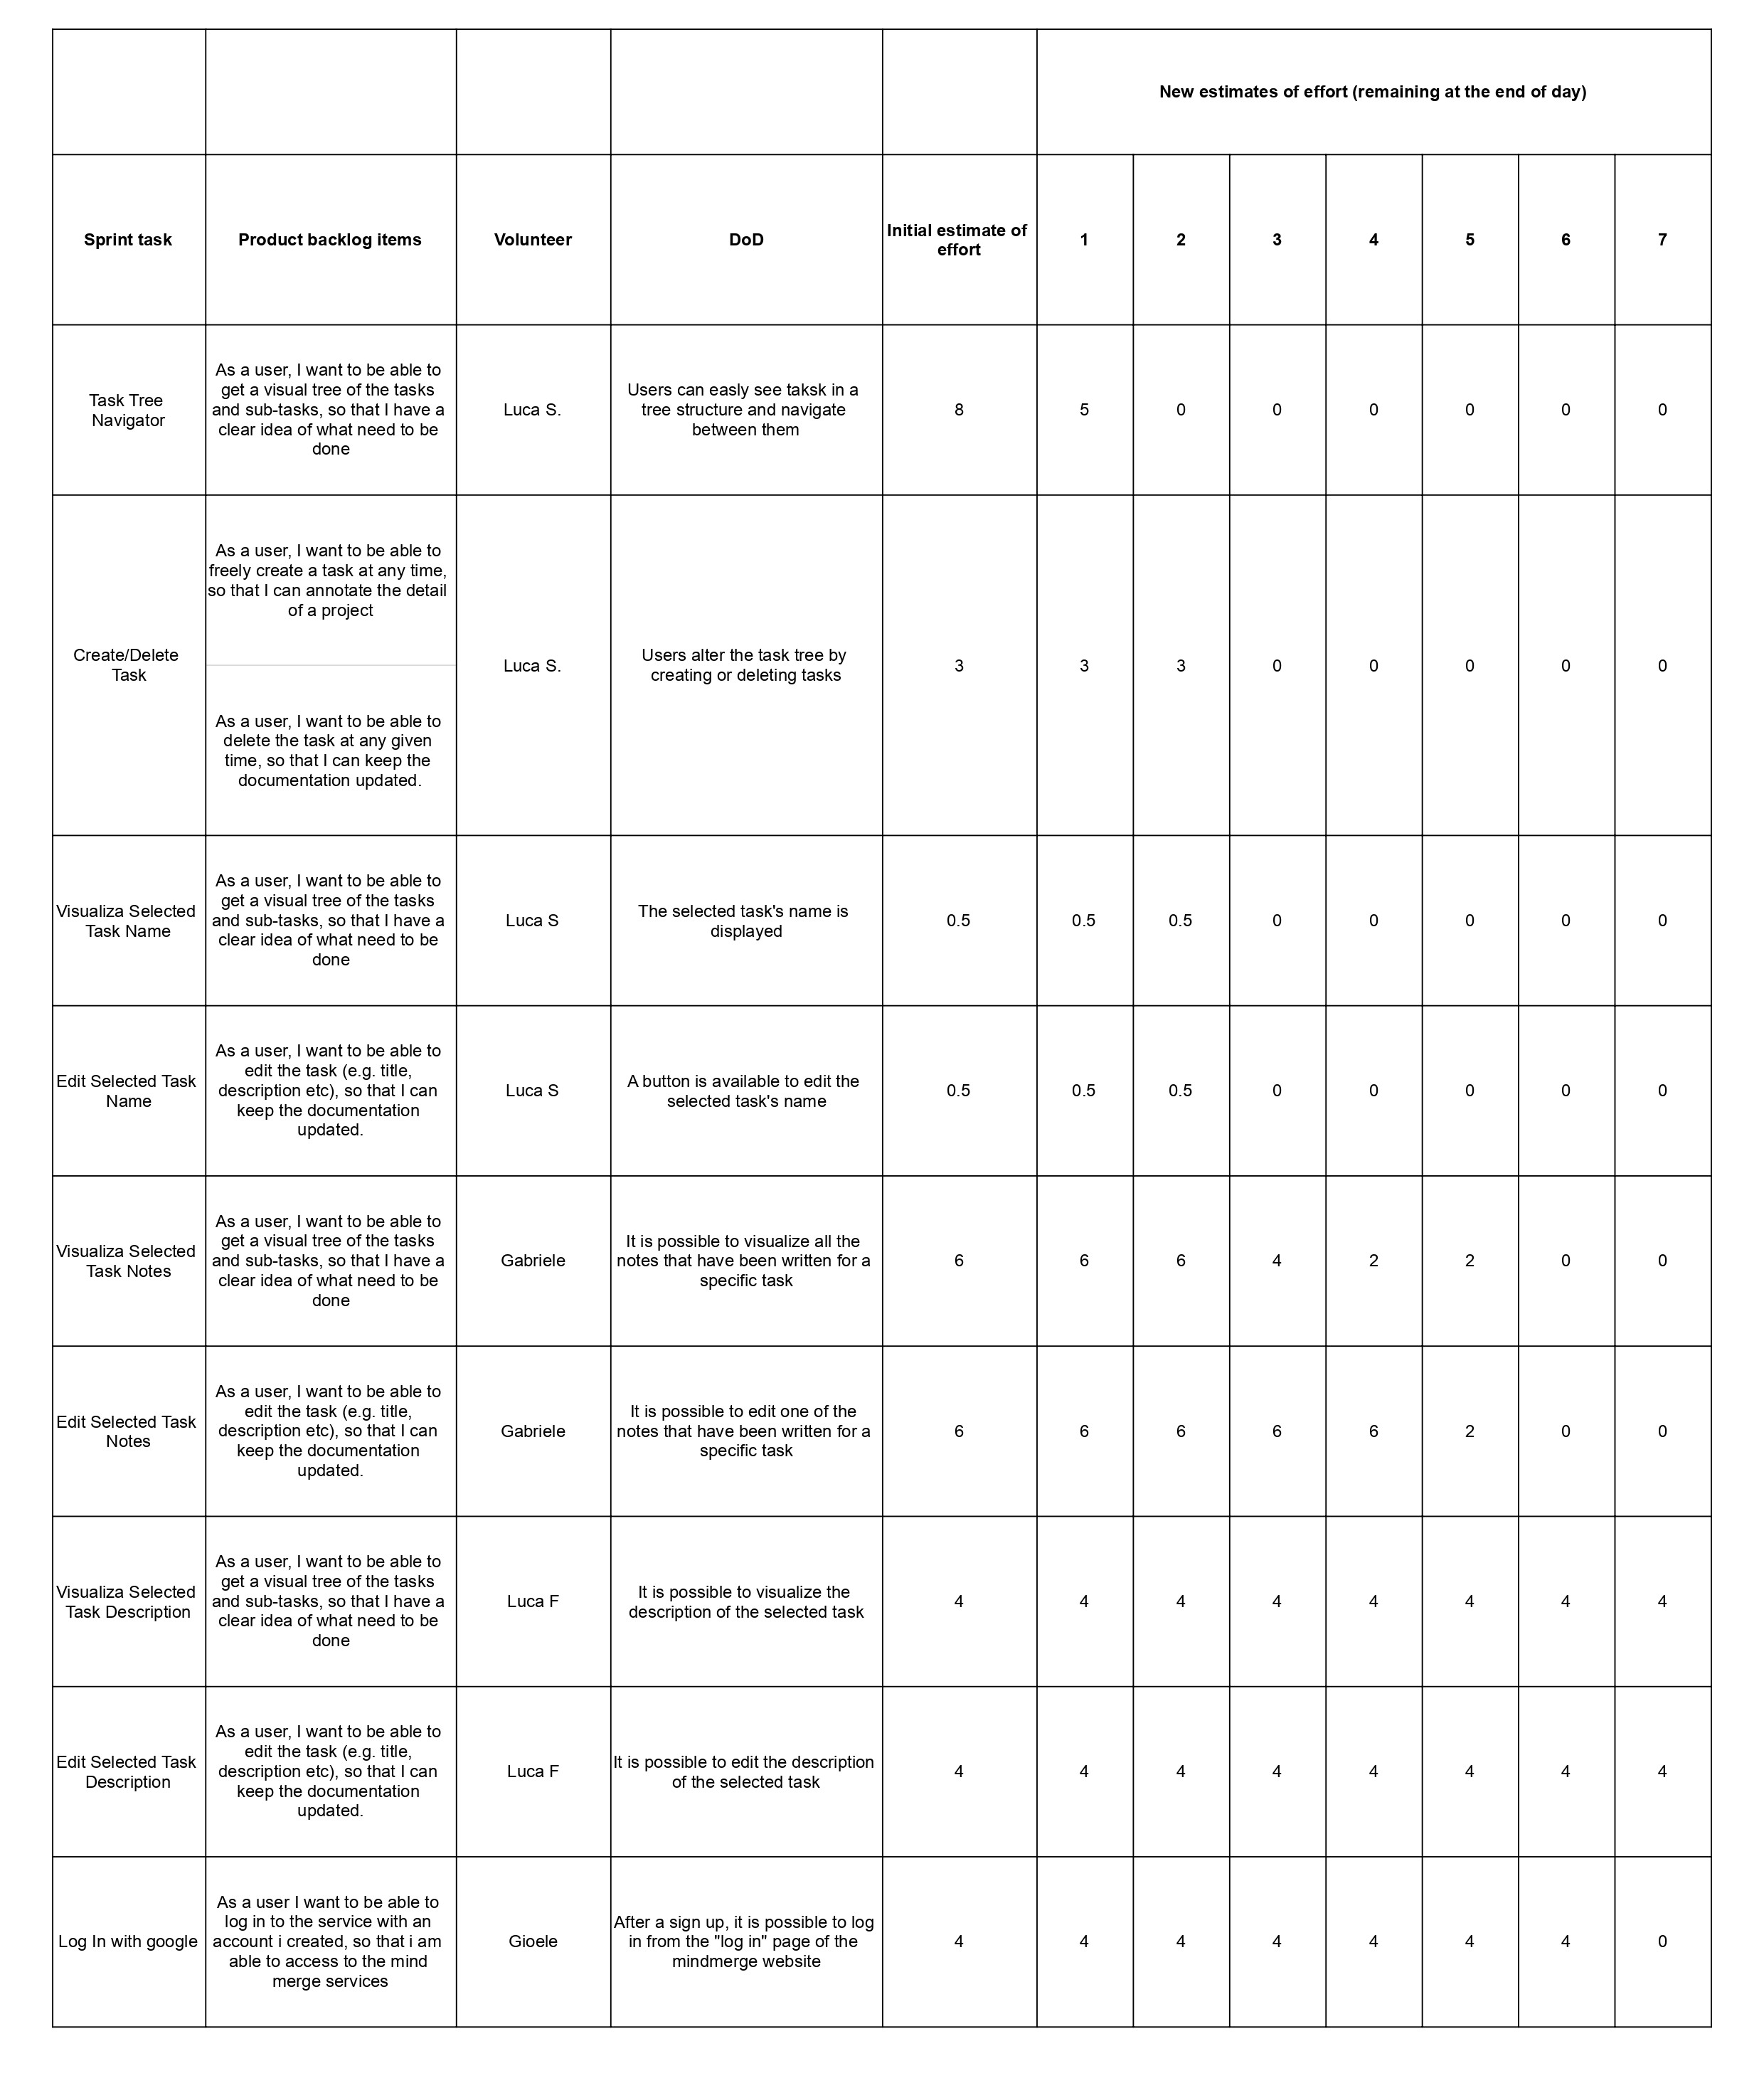
\includegraphics[width=0.95\textwidth]{images/sprint_backlog_3.jpg}

\subsection{Review and Retrospective}
\subsubsection{Retrospective}
\subsubsection{Review}

\subsection{Burn-down Chart}
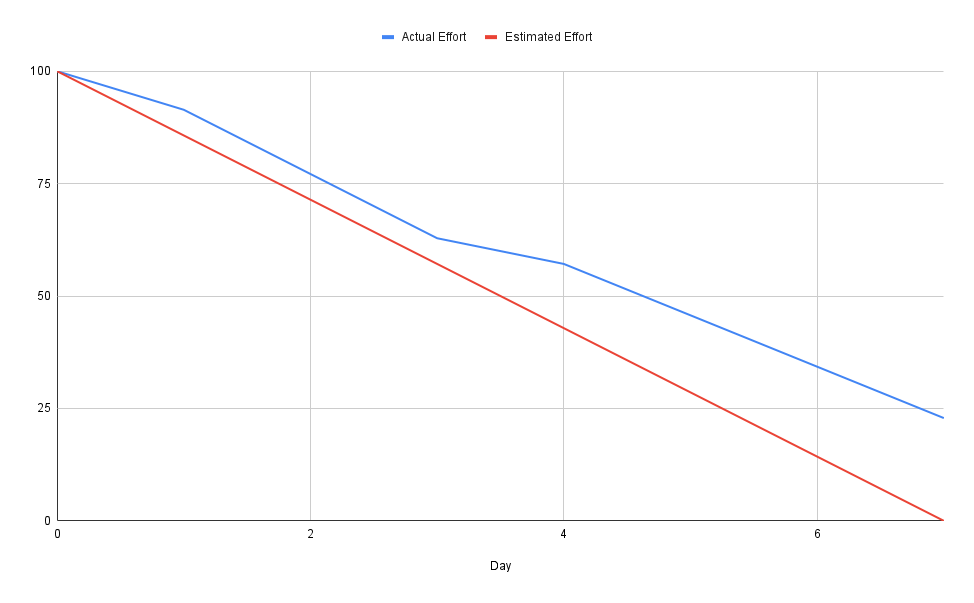
\includegraphics[width=0.95\textwidth]{images/burndown_chart_3.png}
\end{document}
